\documentclass[a4paper, 11pt, oneside]{Thesis}

\usepackage[dvipsnames]{xcolor}

\usepackage[utf8]{inputenc}
\usepackage[T1]{fontenc}
\usepackage{lmodern}

\usepackage[square, numbers, comma, sort&compress]{natbib}

\usepackage{changepage}
\usepackage{float}
\usepackage[section]{placeins}

%\definecolor{rred}{HTML}{e0304e}

\lstset{
  captionpos=b,
  frame=tb,
  comment=[l]{\#},
  basicstyle=\ttfamily\footnotesize\linespread{1.2}\selectfont,
  numberstyle=\footnotesize\color{gray},
  commentstyle=\itshape,
  showstringspaces=false,
  keepspaces=true,
  aboveskip=2em,
  numbers=left,
  escapeinside={<@}{@>},
  moredelim=**[is][\color{rred}]{[@}{@]}
}

\usepackage[capitalise,noabbrev]{cleveref}
\crefname{sublstlisting}{Listing}{Listings}
\Crefname{sublstlisting}{Listing}{Listings}
\crefdefaultlabelformat{#2{\scshape #1}#3}
\AtBeginDocument{\DeclareCaptionSubType{lstlisting}}

\usepackage{varwidth}
\usepackage{verbatim}
\usepackage{stmaryrd}
\usepackage{mathtools}
\DeclarePairedDelimiter\set{\lbrace}{\rbrace}
\DeclarePairedDelimiter\bbrackets{\llbracket}{\rrbracket}
\DeclarePairedDelimiter\angles{\langle}{\rangle}
\DeclarePairedDelimiter\ttangles{\mathtt{<}}{\mathtt{>}}
\newcommand{\univ}{\ensuremath{\mathbb{U}}}

\usepackage{bussproofs}
\def\labelSpacing{1em}
\usepackage[altpo,epsilon]{backnaur}
\newcommand{\bnfmor}[1]{\bnfmore{\hspace{-1.5em}\ooalign{|\cr\hspace{1.5em}}#1}}

\usepackage{tipa}
\newcommand{\ipa}[1]{{\usefont{T3}{cmr}{m}{n}\selectfont#1}}

\usepackage{tikz}
\usetikzlibrary{chains,shapes,arrows,calc,positioning}
\tikzstyle{arrow} = [draw, -latex']
\tikzstyle{box} = [rectangle, draw=black!50, align=left, font={\ttfamily}]
\tikzstyle{init} = [circle, draw=black!50]
\tikzstyle{circ} = [circle, font={\ttfamily}]

\usepackage{siunitx}
\usepackage{csvsimple}
\usepackage{pgfplots}
\pgfplotsset{compat=1.9}
\usepackage{pgfplotstable}
\usepackage{xstring}
\pgfplotsset{where/.style 2 args={
    x filter/.code={
      \IfStrEq{\thisrow{#1}}{#2}{}{\def\pgfmathresult{}}
    }
  }
}

\usepackage{afterpage}
\usepackage{longtable}
\usepackage{amssymb}% http://ctan.org/pkg/amssymb
\usepackage{pifont}% http://ctan.org/pkg/pifont
\usepackage{comment}
\usepackage{algorithm}
\usepackage{algpseudocode}
\usepackage[newfloat]{minted}
\usepackage{physics}
\usepackage{caption}

\graphicspath{{figures/}}
\def\datapath{data}

\begin{document}

\frontmatter
\newcommand{\cmark}{\ding{51}}%
\newcommand{\xmark}{\ding{55}}%
\newcommand {\R}{\mathbb{R}}

%TC:macro \suhrid [ignore]
%\newcommand{\suhrid}[1]{\textcolor{blue}{\textsc{Suhrid:} \textbf{#1}}\par}

%TC:macro \tawfiq [ignore]
%\newcommand{\tawfiq}[1]{\textcolor{red}{\textsc{Tawfiq:}
%\textbf{#1}}\par}

%TC:ignore
\university{{The University of Melbourne}}
\UNIVERSITY{{THE UNIVERSITY OF MELBOURNE}}
\department{{School of Computing and Information Systems}}
\school{{Faculty of Engineering and IT}}
\degree{{Master of Computer Science}}
\title{{Hybrid Horizontal Autoscaling for SLA Compliant Edge Computing Applications}}
\shortauthors{{Suhrid Gupta}}
\authors{
  \texorpdfstring{\href{mailto:suhrid.gupta@student.unimelb.edu.au}{\shortauthornames}}{\shortauthornames}\\
  \small Student Number: 1313675
}
\supervisor{{Dr.~Tawfiq Islam and Prof.~Rajkumar Buyya}}
\addresses{\deptname\\\univname}
\date{June 2024}
\subject{}
\keywords{}
%TC:endignore

%TC:envir lstlisting [option:text] xall
%TC:ignore
%\wordcount{\input{|"bash ./Scripts/FMT-TexCount \jobname.tex"}}
%TC:endignore

\maketitle

\setstretch{1.3}

\fancyhead{}
\rhead{\thepage}
\lhead{}

\pagestyle{fancy}

%TC:ignore
%\quotepage{
%If you aren't sure which way to do something,\\
%do it both ways and see which works better.
%}{
%John Carmack
%}

%\addtotoc{Abstract}  % Add the "Abstract" page entry to the Contents
\abstract{
\addtocontents{toc}{\vspace{1em}}  % Add a gap in the Contents, for aesthetics

Edge computing decentralizes computing resources, allowing for novel applications in domains such as the Internet of Things (IoT) in healthcare and agriculture by reducing latency and improving performance. This decentralization is achieved through the implementation of micro-service architectures, which require low latencies to meet stringent service level agreements (SLA). While cloud computing offers the large data storage and computation resources necessary to handle peak demands, a hybrid cloud and edge environment is required to ensure SLA compliance. This is achieved by sophisticated orchestration strategies such as Kubernetes, which help facilitate resource management. The orchestration strategies alone do not guarantee SLA adherence due to the inherent delay of scaling resources. Existing auto-scaling algorithms have been proposed to address these challenges, but they suffer from performance issues and configuration complexity. In this thesis, a novel auto-scaling algorithm is proposed for SLA-constrained edge computing applications. This approach combines a Machine Learning (ML) based proactive auto-scaling algorithm, capable of predicting incoming resource requests to forecast demand, with a reactive autoscaler which considers current resource utilization and SLA constraints for immediate adjustments. The algorithm is integrated into Kubernetes as an extension and its performance is evaluated through extensive experiments in an edge environment with real applications. The results demonstrate that existing solutions have an SLA violation rate of up to 17\%, whereas the proposed hybrid solution outperforms the baselines and has an SLA violation rate of 6\%, ensuring stable SLA compliance across various applications.

}
%
% Guidelines as of 2019/06/04
% https://gradresearch.unimelb.edu.au/__data/assets/pdf_file/0004/2027839/Preparation-of-GR-theses-rules.pdf
%
\Declaration{

I, \shortauthornames, declare that this thesis titled, ``Enhanced SLA Compliance in Edge Computing Applications through Hybrid Proactive-Reactive Autoscaling'' and the work presented in it are my own. I confirm that:

\begin{itemize} 
\item[\tiny{$\blacksquare$}] this thesis does not incorporate without acknowledgement any material previously submitted for a degree or diploma in any university; and that to the best of my knowledge and belief it does not contain any material previously published or written by another person where due reference is not made in the text.

\item[\tiny{$\blacksquare$}] this thesis did not require clearance from the University's ethics committee.

\item[\tiny{$\blacksquare$}] the thesis is approximately \num[group-separator={,}]{24000} words in length (excluding text in figures, tables, code listings, bibliographies, and appendices).

\end{itemize}
}
{}
\clearpage
%
% Guidelines as of 2019/06/04
% https://gradresearch.unimelb.edu.au/__data/assets/pdf_file/0004/2027839/Preparation-of-GR-theses-rules.pdf
%
\Preface{
Section~\ref{subsec:ch2-k8s-overview} of the thesis which provides an overview of Kubernetes was modified from the research proposal that was undertaken in partial fulfillment of the requirements of the \degreename.\par
All work written by myself in support of this thesis was independently reviewed by my supervisors, \supname. Feedback was also received from my supervisors throughout the creation of the thesis and was incorporated into the final version.

\hiddensection{Publications}
\begin{table}[h!]
    \centering
    \begin{tabular}{p{3cm}p{6cm}p{4cm}}
        \toprule
        \textbf{Authors} & \textbf{Title} & \textbf{Venue}\\
        \midrule
        \multirow{2}{3cm}[-3em]{Suhrid~Gupta, Tawfiq~Islam, Rajkumar~Buyya} & SLA-Driven Hybrid Autoscaling for Edge Computing: Foundations, Review, and Future Directions & ACM Computing Surveys (in submission)\\\\
         & A Hybrid Reactive-Proactive Autoscaling Approach for Microservice Applications in Edge Computing Environments & Journal of Systems and Software (in submission)\\
        \toprule
    \end{tabular}
\end{table}

}
\clearpage
\acknowledgements{
\addtocontents{toc}{\vspace{1em}}  % Add a gap in the Contents, for aesthetics

I wish to thank my primary supervisor, Dr. Tawfiq Islam for his generous and invaluable support, feedback, patience, and guidance throughout the whole research process. His continuous encouragement and insights, both personal and professional, has made an immeasurably impact on me throughout my two semesters working under his supervision. I further wish to thank my co-supervisor Prof. Rajkumar Buyya. His guidance in helping me to set up milestones ensured I met my research deadlines. I am grateful to have had them both as my supervisors, and this research thesis would not have been possible without their support.\par

I further wish to thank my friends and family for their selfless help and constant support throughout my time here at The University of Melbourne, for always motivating me, and for their endless guidance which has helped me complete this research project.\par

}

\tableofcontents
\listoffigures
\listoftables
\lstlistoflistings
\listofalgorithms
%TC:endignore

\addtocontents{toc}{\vspace{1em}}

\mainmatter	
\pagestyle{fancy}
\setstretch{1.5}

\clearpage

\def\chaptertitle{Introduction}

\lhead{\emph{\chaptertitle}}

\chapter{\chaptertitle}
\label{ch:introduction}

In this chapter, a brief overview of the edge computing architecture paradigm, along with its uses, benefits, and challenges with respect to resource scaling are provided in section \ref{sec:edge-arch}. These challenges lead to the research gap and questions this thesis intends to answer in section \ref{sec:problem-overview}.\par

\section{Edge Computing Overview}
\label{sec:edge-arch}

Cloud computing architectures leverage the on-demand accessibility of the Internet. The cloud applications utilize the vast resources of the cloud to perform a task, and relinquish it once it is complete for the other sub-modules in the application to request \cite{rimal2009taxonomy}. In the early days, a singular end-point would be used to access these services, however nowadays the architecture is multi-regional allowing effortless access from across the world. This was achieved through the use of content delivery networks (CDN) located in several regions to allow for data to be quickly replicated and served to clients. This architecture model allows for the processing of large-scale data in a near real-time manner.\par

During the early twenty-first century, this architecture paradigm dominated the Information Technology (IT) industry. Compared to traditional monolithic architectures, the ease of deployment, scalability, coupled with the economic benefits ensured its dominance. The increasing popularity of hand-held devices as well as home appliances has resulted in data being largely produced at the edge of the cloud network. Thus, processing this large amount of data solely on the cloud proved to be an inefficient solution due to the bandwidth limitations of the network \cite{shi2016edge}. Thus, edge computing paradigms were built on the previous foundation of CDNs \cite{satyanarayanan2017emergence}. Edge computing architectures ensure data processing services and resources exist at the peripheries of the network \cite{cao2020overview}. The architecture extends and adapts the computing and networking capabilities of the cloud to meet real-time, low latency, and high bandwidth requirements of modern agile businesses.\par

Edge computing deploys several lightweight computing devices known as cloudlets to form a ``mini-cloud'' and places them in close proximity to the end-user data \cite{liu2019survey}. This reduces the latency in terms of client-server communication and data processing. Figure \ref{fig:edge-architecture-overview} shows a high-level overview of this architecture. Cloudlets can also be easily scaled depending on the resource requirements per edge architecture \cite{ren2019survey}. However, due to the dynamic resource requirements which may fluctuate from time to time, the resources allocated to cloudlets must be dynamically scaled too. This dynamic scaling, along with the inherent latency present between the cloud layer and the edge cloudlets, poses a significant problem to real-time resource scaling \cite{varghese2016challenges}.\par

\begin{figure}[htb]
    \centering
    \caption{Overview of edge computing architecture}
    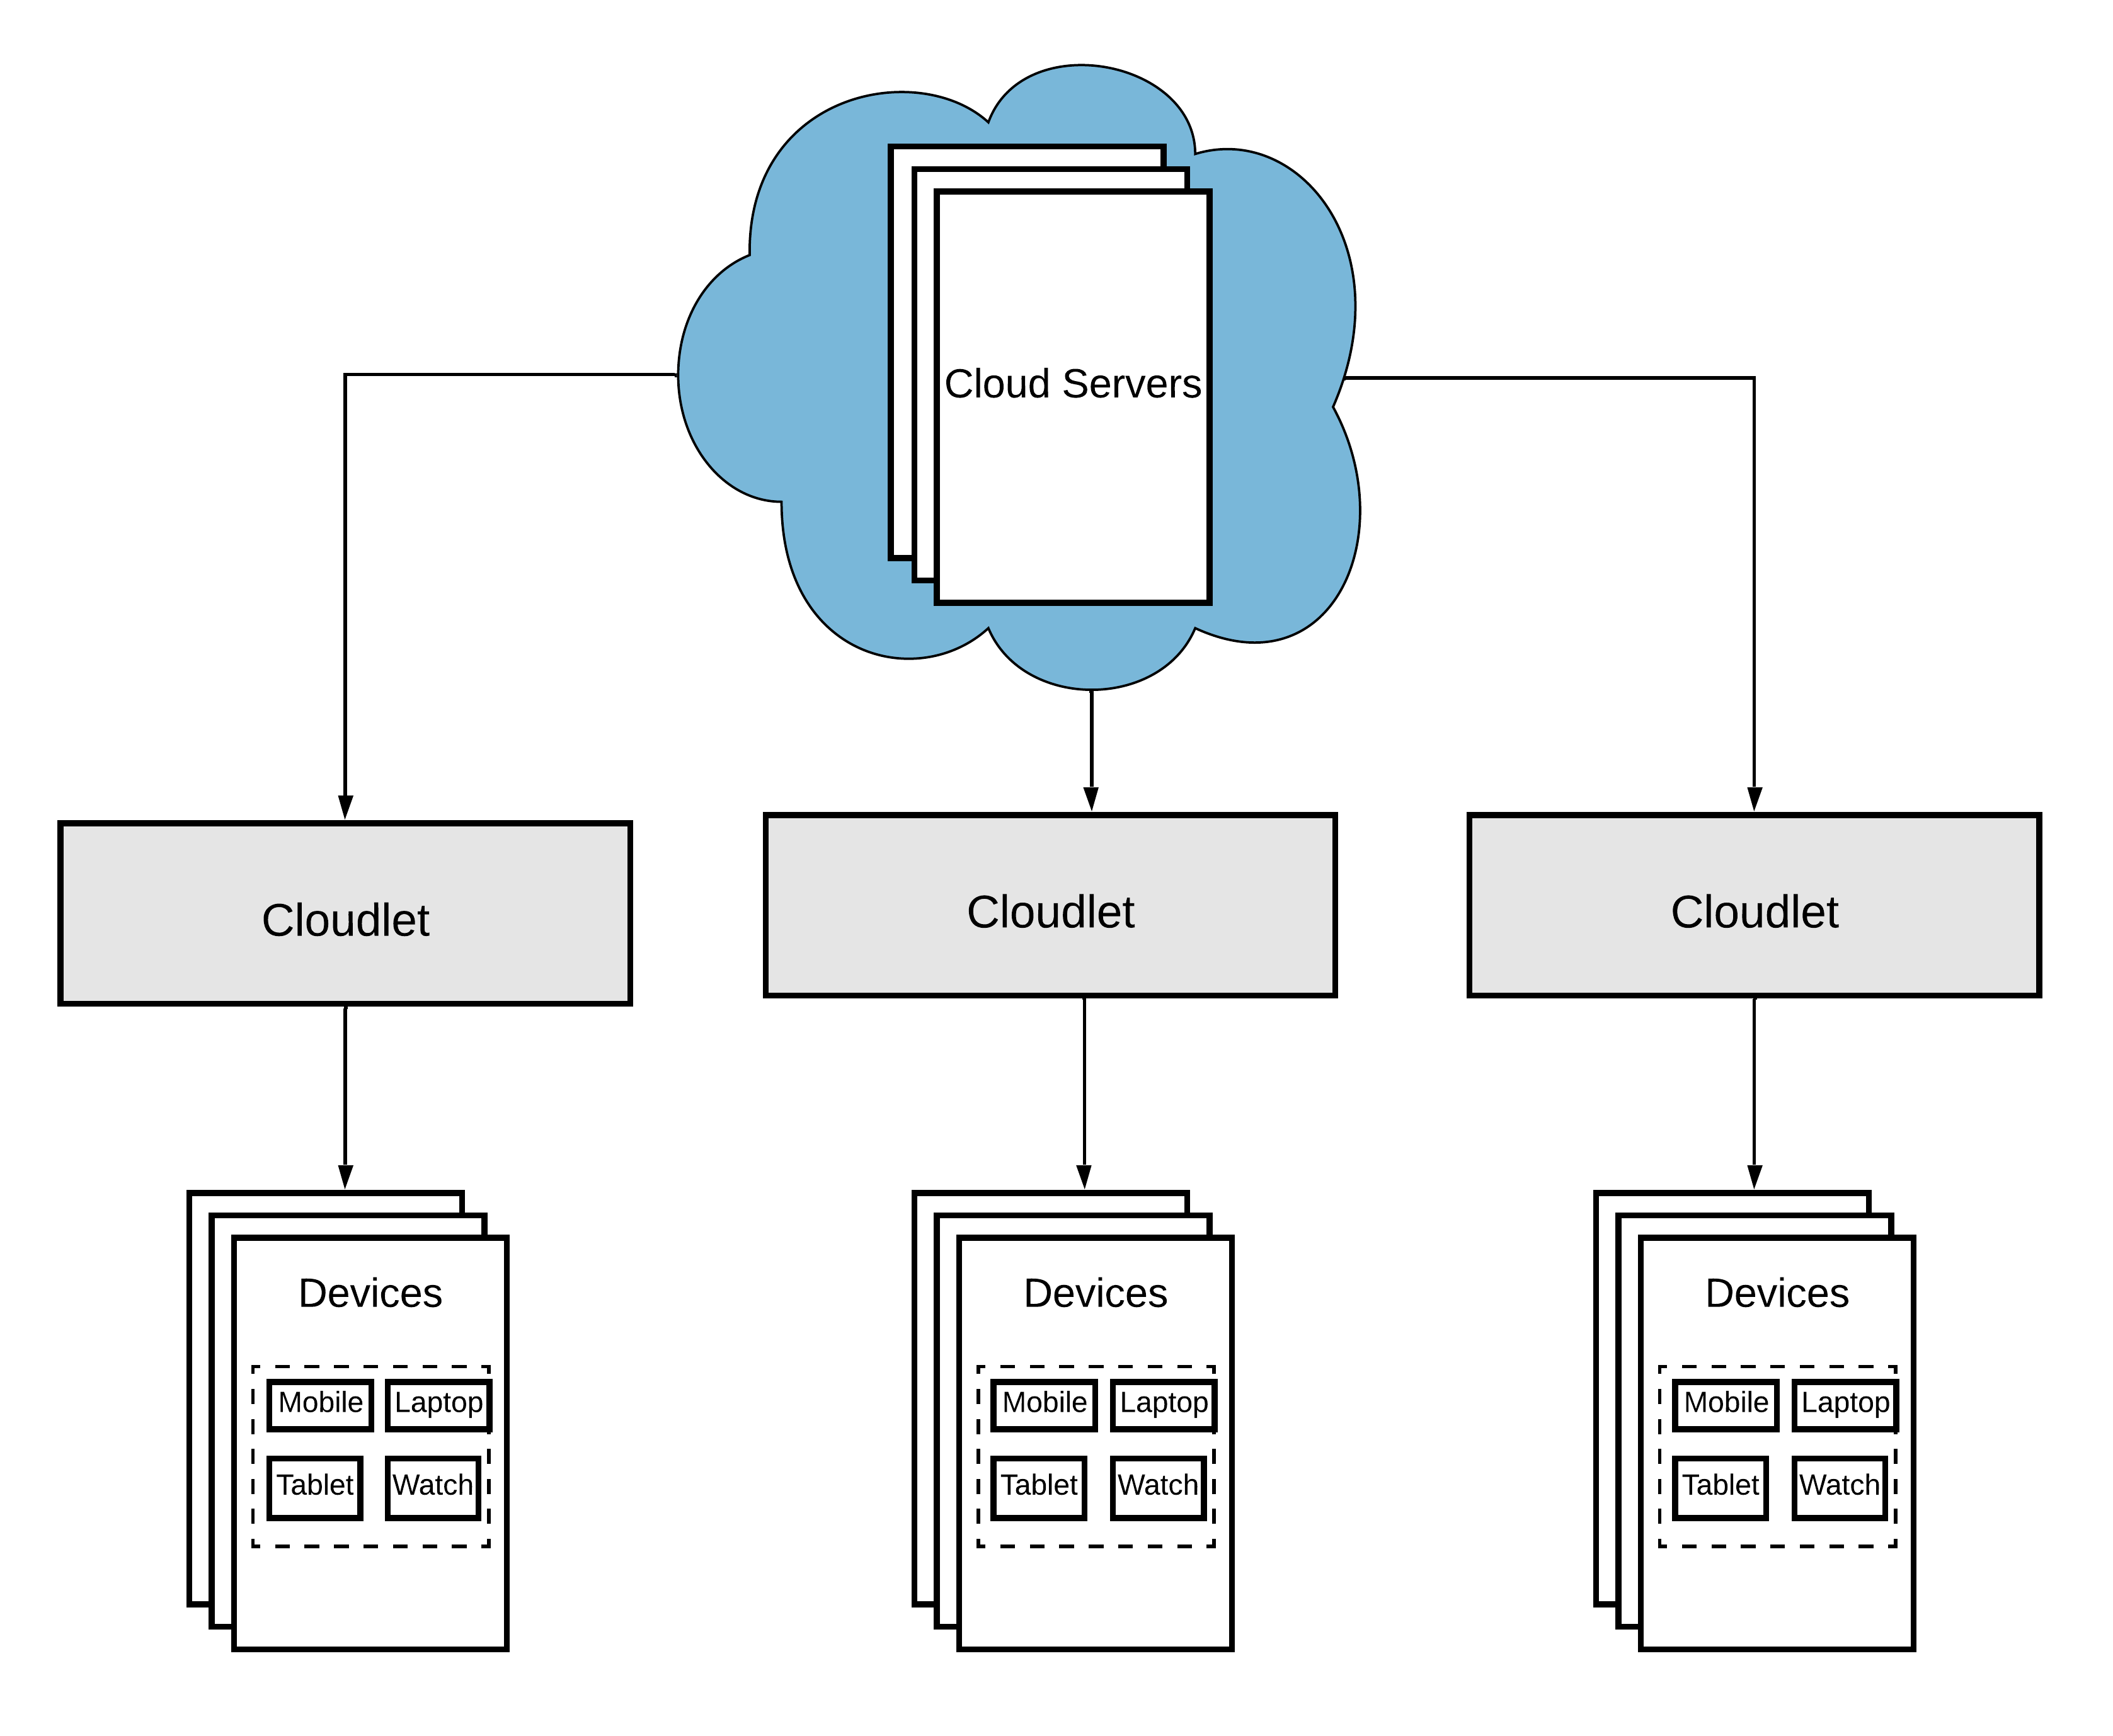
\includegraphics[width=0.9\linewidth]{Figures/Edge-Architecture-Overview.png}
    \label{fig:edge-architecture-overview}
\end{figure}

One method of mitigating this scaling latency is through the use of micro-service applications. By employing a microservice architecture, the resources in a cloudlet are a collection of smaller deployments that are both independent and loosely coupled \cite{villamizar2015evaluating}. This loose coupling ensures that parts of the cloudlet can be scaled as is required, further reducing the time required to scale resources as compared to scaling the cloudlet monolithically.\par

The scaling of these microservice resources is done automatically through a process known as autoscaling. While most microservice applications come bundled with default autoscaling solutions, and these solutions are sufficient for most applications, they fall apart when scaling resources for time-sensitive services such as the ones used in healthcare require stringent compliance to service level agreements (SLA) on metrics such as application latency. This has led to further research on autoscaling solutions for edge computing applications. These primarily fall into two categories. Reactive autoscaling solutions attempt to modify the microservice resource allocation once the required resources exceeds the current allocation. These algorithms are simple to develop and deploy, however the time taken to scale resources leads to a degradation of resource availability and violates SLA compliance \cite{podolskiy2018iaas}. To counteract these pitfalls, proactive autoscaling solutions attempt to model the resource allocation over time and effectively predict the resource requirements. By doing so, the microservice resources can be scaled in advance through a process known as ``cold starting''. This approach removes the latency inherent in scaling resources, however the algorithms are extremely complex to develop, train as well as tune to specific edge applications \cite{straesser2022not}.

\section{Problem Overview}
\label{sec:problem-overview}

With these limitations in mind, the object of this research project was to unify the reactive and proactive autoscaling solutions into a hybrid model. This solution combines the light weight, and ease of use and deployment of the reactive algorithm, with the SLA compliance and accurate resource modelling of proactive ones. The project aimed to answer the following questions in a satisfactory manner:
\begin{itemize}
    \item \textbf{\textit{RQ1:}} Can we integrate reactive and proactive autoscaling methods to develop a tailored algorithm for edge computing that eliminates the requirement for developers to fine-tune hyper-parameters for each autoscaling use case, while being lightweight enough to be deployed and run on cloudlets?
    \item \textbf{\textit{RQ2:}} Can the hybrid autoscaling solution achieve or exceed the SLA compliance capabilities of state-of-the-art reactive and proactive autoscaling solutions for edge computing, while minimizing the degredation of application performance?
\end{itemize}
\clearpage

\def\chaptertitle{Background}

\lhead{\emph{\chaptertitle}}

\chapter{\chaptertitle}
\label{ch:background}

In this chapter, a brief introduction to Service Level Agreements is provided in section \ref{sec:sla}, followed by an overview of microservice architectures is provided in section \ref{sec:micro-svc-arc}. This includes a brief description of the architecture of Kubernetes, along with its scheduling and autoscaling algorithms. Finally, section \ref{sec:lit-review} comprises of a detailed literature review of the state-of-the-art autoscaling algorithms and a comparison of their performances and drawbacks.

\section{Service Level Agreements}
\label{sec:sla}

\begin{figure}[htb]
    \centering
    \caption{Types of service level agreements}
    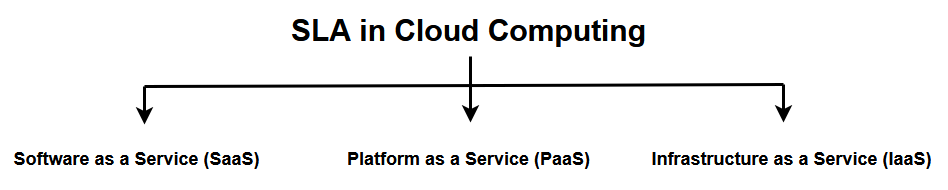
\includegraphics[width=0.9\linewidth]{Figures/SLA-Cloud-Computing.png}
    \label{fig:sla-types}
\end{figure}

Cloud computing generally exposes resource using a pay-as-you-go service. These lucrative plans have led to the implementation of applications and hardwares being delivered as Software as a Service (SaaS), Platform as a Service (PaaS), and Infrastructure as a Service (IaaS). However, consumers of such services have demands which may vary significantly, and it is impossible to fulfill all these expectations. Thus a balance needed to be struck in order to commit to an agreement \cite{patel2009service}. \par
This commitment is known as a Service Level Agreement (SLA). This SLA defines the expected services provided by the provider, and agreed to by the consumer. The most common metric by which SLAs are negotiated between providers and consumers is the availability of service.

\subsection{Availability of Services}
\label{subsec:svc-availability}
Availability is defined to ensure that the functional performance of the edge deployment is maintained for an agreed period. SLAs mostly define either monthly or yearly downtime in order to compute service credits for billing purposes \cite{mirobi2015service}. The downtime can be calculated using the formulae:
%TC:ignore
\[ downtime_{monthly} = \frac{100 - Availability\%}{100} * 30 * 24 \]
\[ downtime_{yearly} = \frac{100 - Availability\%}{100} * 365 \]
%TC:endignore
Table \ref{table:sla-availability} shows the expected down-times for several SLA availability percentages.

%TC:ignore
\begin{table}
    \caption{Summary of SLA availability}\label{table:sla-availability}
    \centering
    \begin{tabular}{|l|l|l|}
        \hline
        Availability \% & Monthly Downtime & Yearly Downtime\\
        \hline
        90\% & 72 hours & 36.5 days\\
        99\% & 7.2 hours & 3.65 days\\
        99.9\% & 43.8 minutes & 8.76 hours\\
        99.99\% & 4.38 minutes & 52.56 minutes\\
        99.999\% & 25.9 seconds & 5.26 minutes\\
        \hline
    \end{tabular}
\end{table}
%TC:endignore

\section{Microservice Architecture}
\label{sec:micro-svc-arc}

Microservice architectures involve decomposing an application into several loosely coupled services, and deploying them on separate servers known as ``nodes''. These services communicate with each other through a lightweight framework such as RESTful APIs \cite{li2021understanding}. Within these services, application data and commands are stored and executed within ``containers''. Typically, these architectures provide scalability, as well as ease of deployment and modification. Availability however, remains an important concern for such deployments. For a deployment to be classified as ``highly available'', it must be accessible at least 99.999\% of the time. For example, a highly available search engine would only face 5 minutes of down time per year \cite{nabi2016availability}. Therefore, an orchestration mechanism is required to manage the deployment and communication of these containers.\par

\begin{figure}[htb]
    \centering
    \caption{Features of Container Orchestration}
    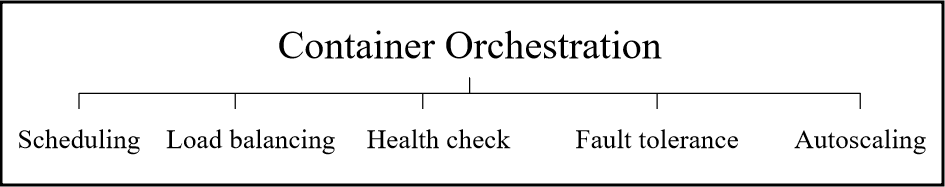
\includegraphics[width=0.9\linewidth]{Figures/Container-Orchestration.png}
    \label{fig:container-orchestration}
\end{figure}

Container orchestration allows the microservice application to customize how the deployment, monitoring, and controlling functions \cite{casalicchio2019container}. Figure \ref{fig:container-orchestration} depicts the typical features of container orchestration.\par
\textit{Scheduling} defines the rules on the number of containers to be executed at any given time. Scheduling also places containers on specific nodes based on availability and best performance.\par
\textit{Load balancing} distributes the resource usage among multiple microservice nodes. By default, a round-robin policy is implemented, although more complex policies may be implemented at the discretion of the developer.\par
\textit{Health checks} ensure that the container is still capable of responding to queries. Typically, these are done using a periodic light-weight HTTP request and verifying the response.\par
\textit{Fault tolerance} maintains several replicas of containers, a strategy commonly used to achieve the high availability mentioned above. Health checks are used to ensure the replicas are functioning, and they typically have strategies to ensure there is no mismatch in data between two fault tolerant containers.\par
\textit{Autoscaling} is the process of automatically adding or removing resources or containers. Internal metrics such as CPU usage are typically used, however custom policies can also be implemented at the discretion of the developer.\par

\subsection{Kubernetes Architecture}
\label{subsec:k8s-overview}

Kubernetes \footnote{\url{https://kubernetes.io/}} is one of the most popular open-source container orchestration platforms \cite{vayghan2019kubernetes}. Initially referred to as ``Borg'', the project was used internally at Google to deploy the majority of their cloud applications before becoming an open-source application \cite{burns2016borg}. Figure \ref{fig:k8s-arch} shows the high-level architecture. The Kubernetes deployment has a controller / worker architecture. The nodes in the Kubernetes cluster are split into either \textit{control plane nodes} and \textit{data plane nodes}. The \textit{control plane nodes} have a collection of processes which help monitor and maintain the desired state of the deployment. The \textit{data plane nodes} contain processes which run the containers doing the actual work, and are managed by the control plane.\par
The smallest unit of work in a Kubernetes deployment is known as a \textit{pod} \cite{baier2017getting}. This is a collection of containers sharing an IP address and port. In summary, microservice architectures are said to be containerized and deployed on Kubernetes in the form of pods \cite{vayghan2019kubernetes}.\par
\begin{figure}[htb]
    \centering
    \caption{Kubernetes Architecture}
    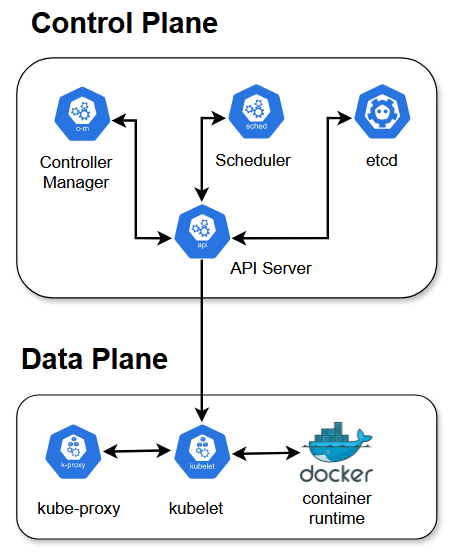
\includegraphics[width=0.5\linewidth]{Figures/K8s-Architecture.png}
    \label{fig:k8s-arch}
\end{figure}

\subsubsection{Data Plane}
\label{subsubsec:k8s-data-plane}

The \textit{container runtime} is a process which downloads or ``pulls'' the image for the required container onto the node. Kubernetes supports a wide range of runtimes, but some of the popular solutions are CRI-O \footnote{\url{https://cri-o.io/}}, containerd \footnote{\url{https://containerd.io/}}, and Docker \footnote{\url{https://www.docker.com/}}.\par

The most important process running on every data plane node is the \textit{kubelet}. This process executes the image assigned to the node via the container runtime, perform health checks, and reports the node status to the control plane.\par

Another data plane process is the \textit{kube-proxy}, which manages the rules for forwarding requests to services, as well as the IP tables of nodes. If a service is added or removed, kube-poxy updates the IP table accordingly.\par

\subsubsection{Control Plane}
\label{subsubsec:k8s-control-plane}
The \textit{API Server} is the primary communication endpoint for the entire deployment. Every component in the architecture communicates through it to exchange information. It is also used to update the current deployment state. The API Server is a simple RESTful API implementation, exposing well-documented APIs for access by other components as well as developers. Multiple replicas of this component are typically maintained to ensure high availability.\par

The \textit{etcd} is a data store which persists the deployment state in a key-value format. The data is serialized unlike in the stateless API server. This data adheres the properties of \textit{recovery} and \textit{availability}. \textit{Recovery} ensures that any corruption of data is reverted using a system of backups such as checkpoints. \textit{Availability} ensures that the deployment is reachable by the end-user regardless of the traffic being requested on the network.\par

\textit{Controller Manager} implements the desired deployment state. During initial deployment, the controller manager inputs the required workload as the desired state, after which it continually monitors the deployment state using a system of looping controls. If the deployment requires modifications, they are achieved using the API server, and the deployment is brought back into alignment with the desired state.\par

Finally, the \textit{scheduler} decides the location where the pod will be deployed. The scheduler runs a control loop which searches for uncheduled pods using the API server. It then assigns the pods to a dataplane node based on several predicates and priorities such as resource requirements and node affinity respectively.

\section{Autoscaling Overview}
\label{sec:autoscaling}

Apart from intelligently scheduling pods to data plane nodes \cite{kayal2020kubernetes}, Kubernetes has the provisions to dynamically respond to changes in resource requirements. This process of scaling nodes, pods, or other resources depending on requirements in an automated manner is known as \textit{autoscaling}. Kubernetes supports three variations of autoscaling.\par

\textit{Cluster autoscaling} modifies the number of nodes running in the entire deployment, or cluster. Dynamically allocating nodes based on resource requirements helps to manage the cost of running Kubernetes deployments on external platforms such as Amazon \footnote{\url{https://docs.aws.amazon.com/eks/}} or Google \footnote{\url{https://cloud.google.com/kubernetes-engine/}}. The autoscaler works by looping through two tasks. The first watches for unscheduled pods, the second checks if the current deployed pods (pods which are running on the data plane) can be merged on a smaller number of nodes.\par

\textit{Vertical pod autoscaling} modifies the CPU and memory resources assigned to pods. By default, the scheduler reserves a larger amount of these resources to pods than is usually required. By performing vertical pod autoscaling, the cluster can better manage its over-provisioned resources in real-time.\par

\textit{Horizontal pod autoscaling} is the most commonly used autoscaling strategy \cite{baresi2021kosmos}, it modifies the number of pods assigned to a task, based on the resources being requested. Kubernetes implements this using a periodic control loop which runs every 15 seconds by default. The control manager compares the actual resource utilization with the target utilization defined by the deployment script, and scales the number of pods accordingly.

\subsection{Custom Autoscaling}
\label{subsec:custom-autoscaling}

The default horizontal pod autoscaler uses pod CPU and memory utilization when making its scaling decisions. However, these metrics may be too rigid when it comes to edge architectures \cite{coulson2020adaptive}. The strict SLA constraints in place, along with the lower amount of resources present in the edge layer as compared to the cloud layer, make it imperative for custom metrics to be employed to autoscale resources as efficiently as possible.\par

Figure \ref{fig:custom-autoscale-overview} depicts the general architecture of the custom autoscaler. Typically, the autoscaler queries metrics from the default metrics registry, which acts as a central store for all metrics that are exposed to the developer. Three interfaces to this registry are exposed:
\begin{itemize}
    \item \textit{Resource metric API} is used to access predefined metrics such as CPU and memory resources of both pods as well as nodes.
    \item \textit{Custom metric API} contains user-defined custom metrics associated with all Kubernetes objects.
    \item \textit{External metrics API} contains metrics of objects which are not associated with Kubernetes.
\end{itemize}
For custom metric autoscaling, the autoscaler must be configured in a way where the metrics can be fetched from the custom metric API. This is done by configuring the custom metric server, several frameworks to simplify this process such as the Kubernetes Instrumentation SIG \footnote{\url{https://github.com/kubernetes/community/tree/master/sig-instrumentation}} exist which simplify the server building process.

\begin{figure}[htb]
    \centering
    \caption{Custom Autoscaler Architecture Overview.}
    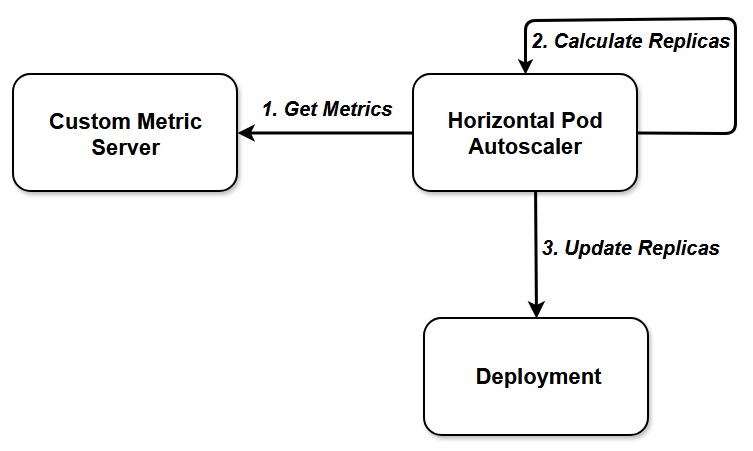
\includegraphics[width=.7\linewidth]{Figures/Custom-Metrics-Autoscaling.png}
    \label{fig:custom-autoscale-overview}
\end{figure}

\section{Literature Review}
\label{sec:lit-review}

In this section, we discuss some of the common challenges and limitations inherent in an edge computing paradigm, before delving into the many attempts at mitigating them.

\subsection{Edge Computing Issues and Challenges}
\label{subsec:edge-issues}

\subsubsection{Resource Allocation}
\label{subsubsec:edge-resource-alloc}

Cao et al. \cite{cao2020overview} demonstrated the key differentiations traditional cloud computing architectures have compared to edge architectures, while asserting that edge deployments remain an extension of the cloud. The aim of cloud computing infrastructures is to process huge amounts of data from multi-regional zones, or in the best case, globally. This is done so as to perform in-depth analysis in diverse fields such as health-care, robotics, and business decision making. Traditionally, they also dealt with non-real-time data for decision-making \cite{premsankar2018edge}. On the other hand, edge computing usually handles smaller scale data, locally clustered and isolated in separate zones, and highly real-time in nature \cite{mishra2020early}. The data processed in traditional cloud computing environments are also generally done using a high network bandwidth. This is due to the large distances data needs to be transmitted over to reach the data centres and cloud servers. Such data transmission places an enormous burden on the cloud network, and poses multiple security challenges in ensuring that the data is not compromised in transit.\par

The real-time nature of edge computing applications necessitates a method of resource allocation which ensures minimal cost of deployment, and maximum efficiency in terms of performance. As mentioned in section \ref{sec:edge-arch}, micro-service container orchestration technologies are leveraged to achieve these aims. Kristiani et al. \cite{kristiani2019} demonstrated an edge computing architecture, where the edge layer consists of Kubernetes nodes. Such a deployment increases the scalability, as well as maintains the ease of deployment, upgrade, and removal of nodes in the edge layer. Scaling of resources through the means of autoscaling depending on the resource requirements is crucial to the architecture's performance. Default solutions such as the inbuilt autoscaler provided by Kubernetes, while generally useful for cloud applications, are unsuitable for edge architectures according to Phan et al. \cite{phan2022traffic}. They note that due to the algorithm's default nature to allocate resources in a round-robin manner, they do not take into account which Kubernetes nodes require resources the most, violating edge architecture paradigms.

\subsubsection{Cold start problem}
\label{subsubsec:cold-start}

To explain the cold start problem, we use the example of horizontal pod autoscaling in Kubernetes. When the control plane requests for a deployment to be scaled up, Kubernetes adds more pods to the dataplane nodes.  Based on the internal workload, the pod needs to be elastically scaled out \cite{beni2021reducing}. Even though the pod start up time is significantly quicker than, say, a traditional virtual machine, there is a latency inherent to bootstrapping the container, preparing the pod environment based on the deployment specification, and initialising the code present in the container image, and registering the pod in a ``ready'' state to the Kubernetes control plane. This latency inherent when scaling resources is known as the ``cold start''.\par

Several techniques exist to reduce this cold start latency. The Kubernetes container runtime uses snapshots \cite{cadden2019seuss}, lazy fetching of container images \cite{lorenzo2019fogdocker}, and container queues \cite{lin2019mitigating}. However, these measures do not eliminate the issue of cold start. Due to this, researchers looked into scaling resources in a predictive manner, so as to ensure the microservice application has enough time to spool up resources before the actual demand comes in.\par

\subsubsection{Service Level Agreements}
\label{subsubsec:sla-edge}

There are several challenges posed in providing SLA guarantees in an edge deployment:
\begin{itemize}
    \item Users queueing for large periods of time to use a service \cite{venticinque2011cloud}
    \item Degradation of application performance due to peak levels of workload, leading to user dissatisfaction \cite{sakr2012sla}
    \item Incorrect resources being allocated to the application, leading to either a degradation of availability, or large cost of application deployment \cite{houlihan2014auditing}
\end{itemize}

Several strategies have been proposed to counteract these challenges. Linlin et al. \cite{wu2013sla} proposed a customer-driven strategy  to minimize the provisioning costs. The algorithm considers the customer profiles as well as cloud providers' quality parameters such as response time to dynamically handle customer requests. Rajkumar et al. \cite{rajavel2012achieving} proposed a solution for alleviating the issue of delay in service allocation to users through the use of a novel hierarchical scheduling algorithm. This algorithm increases the performance of the scheduling algorithm, thus reducing the wastage of resources, and minimizing wait times. Sakr et al. \cite{sakr2012sla} introduced a novel approach to combat application performance degradation by using a middleware between consumers and the cloud. This middleware helps to facilitate dynamic provisioning of cloud databases based on consumer requirements, tailoring their needs and requirements to mitigate peak usages being hit often.

\subsection{Resource Management and Scheduling Solutions}
\label{subsec:resource-schedule-solutions}

To counteract the limitations discussed in section \ref{subsubsec:edge-resource-alloc}, several custom scheduling and resource management algorithms have been proposed for edge architectures.\par

Skarlat et al. \cite{skarlat2016resource} demonstrated an algorithm for resource scheduling where the usage of resources was formalized as an optimization problem. Thus, the authors attempted to minimize the network delay when requesting computational resources. Based on this work, Aazam and Huh \cite{aazam2015dynamic} proposed another solution for resource management which attempted to estimate the resources per service required, based on the user's previous behaviour as well as type of service being requested. By following such an approach, the resource wastage was actively reduced in edge nodes. Another resource allocation solution provided by Ni et al. \cite{ni2017resource} was based on priced timed Petri nets. The resources in the edge nodes are divided into several groups. The users can then select resources as per their requirements in an autonomous manner according to the price and time-cost of the operation.\par

Based on these initial proposals, Nguyen et al. \cite{nguyen2020elasticfog} revealed ElasticFog, a resource provisioning algorithm which operates on top of the Kubernetes architecture. The algorithm provides real-time elastic scheduling for the resources on the edge nodes by monitoring the traffic distribution on the network, thereby achieving a significantly higher throughput and network efficiency in comparison to the default Kubernetes scheduler solution.\par

Wojciechowski et al. \cite{wojciechowski2021netmarks} proposed a similar extension to the Kubernetes scheduler which deployed traffic-aware provisioning of resources. The extension worked alongside the Istio Service Mesh \footnote{\url{https://istio.io/latest/about/service-mesh/}} to collect dynamic network metrics for the scheduling of resources. The algorithm was shown to have highly efficient uses for edge deployments such as the 5G network.\par

While these proposals improved the scheduling and resource provisioning of edge deployments, they did not address key limitations addressed above such as the need for dynamic resource scaling so as to face the challenges of real-time data processing and SLA compliance. Due to these issues, several autoscaling algorithms were proposed to address them.

\subsection{Reactive Autoscaling Solutions}
\label{subsec:reactive-solutions}

Nunes et al. \cite{nunes2021state} stated that horizontal pod autoscaling using a reactive strategy remains the most popular autoscaling technique, as well as research topic. These strategies, despite having limitations such as a reliance on predetermined resource thresholds and a delay in resource scaling, have been popular in research articles.  Dogani et al. \cite{dogani2023auto} stated that this was due to the simplicity and user-friendliness in developing them. Table \ref{tab:reactive-autoscalers} summarizes the reactive autoscaling algorithms discussed below:\par

Kampars and Pinka \cite{kampars2017auto} proposed a reactive autoscaling algorithm for edge architectures based on open-source technologies. The algorithm scales in a non-standard approach, considering real-time adjustments in the application logic to determine the strategy of scaling, resulting in several improvements in performance.\par

Zhang et al. \cite{zhang2019quantifying} presented an algorithm for determining edge elasticity through container-based autoscaling. The authors posit that elasticity is a key factor of how an edge deployment as well as the lightweight containers which make up the edge layer perform. The framework not only autoscales container resources, but also monitors resource usage. They were able to show experimentally that to balance system stability with a decent elasticity required careful tuning of parameters such as the cooldown periods of scaling. \par

\suhrid{Use this justification in my experimental HPA cooldown}

Srirama et al. \cite{srirama2020application} investigated an container-aware autoscaling solution which deploys applications to containers which it deems ``best-fit''. The algorithm also uses a rule-based policy to minimize the deployment time, thus mitigating the issue of cold-start. Finally, a dynamic bin-packing sub-algorithm ensures that the applications are deployed on the least required physical servers, thus minimizing wastage of computing resources. The authors experimentally demonstrated that this algorithm minimized  the processing time, cost, and resource utilization.\par

Hoenisch et al. \cite{hoenisch2015four} implemented a four-fold autoscaling strategy for containerised applications which asks if the containers or servers can be autoscaled horizontally or vertically. This question is formalized as a multi-objective optimization problem, and the approach used reduced the cost of each request by more than 20\%.\par

Santos et al. \cite{santos2020qoe} implemented a quality of experience based autoscaling of containerized edge deployments. The algorithm can autoscale both horizontally and vertically on a set of quality metrics which can be customized by the end-user.\par

Sheganaku et al. \cite{sheganaku2023cost} devised an container-based autoscaling solution which allocates resources in a four-fold manner similar to Hoenisch et al. \cite{hoenisch2015four}. The authors formulated the problem as a multi-objective optimization problem and applied a Mixed-Integer Linear Programming (MILP) approach to allocate resources to containers. Such an approach demonstratively reduced costs while maintaining SLA constraints.\par

Taherizadeh and Stankovski \cite{taherizadeh2019dynamic} proposed a multi-leve autoscaling solution using a rule-based approach. The algorithm uses dynamically changing thresholds based on both the container infrastructure as well as application, resulting in improvied performance as compared to other reactive approaches.\par

Phan et al. \cite{phan2022traffic} proposed a reactive autoscaling solution for edge deployments for IoT devices which dynamically allocates resources based on incoming traffic. This traffic-aware horizontal pod autoscaler (THPA) operates on top of the underlying Kubernetes architecture. As discussed above, the default Kubernetes horizontal pod autoscaler scales resources in a round-robin manner, not taking into context which nodes are receiving the highest resource requests. THPA alleviates this issue by modelling the resource requests per Kubernetes nodes. It then intelligently allocates pods to the nodes with higher number of requests. The authors were able to experimentally demonstrate that following such an approach provided a 150\% improvement in response time and throughput.

\suhrid{@Tawfiq what do you think of this table format? I am a bit worried it is too verbose, as that was one of the feedbacks I got in the research proposal. Do you think I should change the colums to simple ticks and crosses instead?}

%TC:ignore
\begin{longtable}{|m{2em} | m{5em} | m{4em} | m{10em} | m{11em}|}
\caption{Summary of reactive autoscaling solutions}\label{tab:reactive-autoscalers}
\hline
Ref & Technique & Scaling Metrics & Contributions & Limitations\\
\hline
\cite{phan2022traffic} & Rule-based & I/O requests & Traffic aware reactive autoscaling based on which node receives resource requests & Not SLA compliant due to the delay in scaling resources\\
\hline
\cite{kampars2017auto} & Control theory & CPU / Memory & Low / high level metrics integration & Complex and challenging metric selection and integration \\
\hline
\cite{zhang2019quantifying} & Rule-based & CPU & Automated autoscaling for container-based edge environments & Delay in scaling resources\\
\hline
\cite{srirama2020application} & Rule-based & CPU / Memory & Heuristic autoscaling algorithm for microservice deployments & Complex and user-intensive parameter tuning\\
\hline
\cite{hoenisch2015four} & Multi-objective optimization & CPU / Memory & Solves the four-fold optimization problem & Heavy performance and resource overhead when running in edge deployments\\
\hline
\cite{santos2020qoe} & MILP & QoE Metrics & Algorithm that maximizes resource utilization at the lowest cost & Unable to scale well on highly dynamic workloads\\
\hline
\cite{sheganaku2023cost} & MILP & CPU / Memory / QoE Metrics & Cost-effective autoscaling solution using linear programming & Too time consuming and computationally expensive for edge deployments\\
\hline
\cite{taherizadeh2019dynamic} & Rule-based & CPU / Memory & Multi-level autoscaling, leveraging monitoring and dynamic thresholds for better performance & Costly to optimize\\
\hline
\end{longtable}
%TC:endignore

\subsection{Proactive Autoscaling Solutions}
\label{subsec:proactive-solutions}

Lorido et al. \cite{lorido2014review} showed that compared to reactive algorithms, proactive algorithms achieved better resource allocation once they had been carefully optimized. Machine learning (ML) techniques such as auto-regressive integrated moving averages (ARIMA) and long short-term memory (LSTM) have gained populary in time-series analysis due to their relative ease of building and efficiency compared to other ML models. Through the careful use of these models, linear patterns in the data can be automatically identified in a short amount of time with relatively constrained resources. There are however several challenges when implementing a proactive algorithm. Time-series analysis models may struggle when dealing with highly complex and non-linear data \cite{dogani2023auto}. The development of a generalised algorithm for several edge architectures remains a costly process. One of the biggest challenges is the initial lack of training data. Another issue is the exploding or vanishing gradient problem \cite{pascanu2013difficulty}, though modern algorithms ensure that they avoid this pitfall \cite{hochreiter2001gradient}. Despite these challenges, their application in scaling of resources with semi-predictable data series remain valuable. Table \ref{tab:proactive-autoscalers} summarizes the proactive autoscaling algorithms discussed below:\par

Ju et al. \cite{ju2021proactive} presented a proactive horizontal pod autoscaling solution for edge computing paradigms. The algorithm, known as Proactive Pod Autoscaler (PPA) was designed to predict resource requests on multiple user-defined metrics, such as CPU request and I/O traffic requests. The algorithm does not use any specific machine learning model for the time-series analysis, instead the model is to be inputted by the user. This model agnostic architecture allows for a very high level of customization. The user can deploy an ARIMA, LSTM, or even Bayesian confidence models. In a confidence model, the autoscaler will only deploy resources if the confidence value is seen to be above a specified user-defined threshold. The authors validated their findings by testing the architecture using LSTM and ARIMA models, the results concluded that this algorithm significantly outperformed both the default Kubernetes autoscaler, as well as existing reactive autoscaling solutions.\par

\suhrid{The research proposal lit review has a paragraph detailing how this algo works. Use that to describe the proactive part of my own hybrid architecture}

Imdoukh et al. \cite{imdoukh2020machine} proposed a proactive autoscaling solution using an LSTM model, designed for edge computing architectures. The algorithm uses an LSTM neural network to predict future network traffic workload to determine the resources to assign to edge nodes ahead of time (cold-start). The authors experimentally demonstrated that their algorithm was as accurate as existing ARIMA-based proactive solutions, but theirs significantly reduced the prediction time, as well as computed the minimum resource allocation required to handle future workload.\par

\suhrid{This paper has a good description of proactive architecture as well, may consider using this instead}

Messias et al. \cite{messias2016combining} created a proactive autoscaler using genetic algorithms (GA). The genetic algorithm combines several time-series forecasting models, while having the benefit of not requiring a training phase as the model adapts to the incoming data. The experimental results concluded that this approach produces results comparable to several state-of-the-art proactive models, and can adapt to various time series models.\par

Abdulla et al. \cite{abdullah2020burst} devised an autoscaling solution which is capable of detecting sudden bursts in dynamic workloads. The algorithm achieves this through a method of workload and resource prediction to make a scaling decision. Experimenting on several burst-heavy workloads, the autoscaler demonstrated significant improvements compared to other state-of-the-art methods.\par

Alidoost et al. \cite{alidoost2023introducing} proposed a workload classification model using a Support Vector Machine (SVM). The algorithm extracts the user's workload characteristics, and then trains the SVM on it. The authors demonstrated a 10\% forecast error reduction compared to other machine learning proactive forecast approaches.\par

%TC:ignore
\begin{longtable}{|m{2em} | m{5em} | m{4em} | m{10em} | m{11em}|}
\caption{Summary of proactive autoscaling solutions}\label{tab:proactive-autoscalers}
\hline
Ref & Technique & Scaling Metrics & Contributions & Limitations\\
\hline
\cite{ju2021proactive} & User-defined models & User-defined metrics & Fully customizable architecture with user-defined metrics and prediction model & Complex hyper-parameter tuning, lack of initial training data causes erroneous predictions\\
\hline
\cite{imdoukh2020machine} & LSTM & HTTP requests & Proactive autoscaler for edge architectures using an LSTM model & Initial lack of training data leads to erroneous predictions\\
\hline
\cite{messias2016combining} & GA & Response time & Genetic algorithm based proactive autoscaler with no training phase & High rate of initial errors due to GA randomness\\
\hline
\cite{abdullah2020burst} & XGBoost & CPU & Autoscaler capable of burst detection & Incapable of capturing several other workload patterns\\
\hline
\cite{alidoost2023introducing} & SVM & CPU & SVM based workload prediction model & Difficulty in identifying non-linear workload patterns\\
\hline
\end{longtable}
%TC:endignore

\subsection{Hybrid autoscaling solutions}
\label{subsec:hybrid-solutions}

All the approaches mentioned in sections \ref{subsec:reactive-solutions} and \ref{subsec:proactive-solutions} have their benefits and drawbacks. Thus, hybrid solutions which merge multiple autoscaling methods were proposed \cite{qu2018auto}. While hybrid algorithms for cloud-based deployments exist, integrating them into edge architectures pose several challenges due to the lower data storage and computational capacity of the edge layer. Furthermore, extracting the proactive time-series analysis to the cloud layer poses further challenges due to the inherent latency present between the two layers. Despite this, exploring these solutions provides a solid template for the approach used in this paper, table \ref{tab:hybrid-autoscalers} shows an overview of the proposals discussed below:\par

In 2007, one of the first hybrid algorithms for a distributed deployment was proposed by Jing et al. \cite{xu2007use}. This algorithm combined rule-based fuzzy inference with machine learning forecasting for dynamic resource allocation. The authors experimentally verified their algorithm through a prototype to demonstrate that it can reduce the resource consumption on resource management systems compared to their default resource allocation algorithms.\par

Based on this work, Lama and Zhou \cite{lama2009efficient} proposed a resource provisioning algorithm for multi-cluster set ups using a hybrid autoscaler. The autoscaler comprised of a combination of fixed fuzzy rule-based logic and a self adaptive algorithm which dynamically tuned the scaling factor. The authors tested this algorithm on a simulation to demonstrate performance benefits compared to existing approaches.\par

A hybrid approach for cloud computing architectures was proposed by Ramp{\'e}rez et al. \cite{ramperez2021flas}. The algorithm which was called Forecasted Load Auto-scaling (FLAS), combines a predictive model for forecasting time-series resources, while the reactive model estimates other high-level metrics and delegates for the proactive model, reducing the potential forecast error when encountering previously unseen workloads. The approach was shown to demonstrate efficient resource allocation as compared to other state-of-the-art solutions.\par

Finally, Biswas et al. \cite{biswas2017hybrid} presented a hybrid algorithm designed for cloud computing deployments with service level agreements. The proactive algorithm involves a machine-learning based approach using an SVM model, alongside the reactive algorithm to dynamically allocate resources. The algorithm was experimentally shown to perform better than a pure reactive or proactive solution in most cases.\par

%TC:ignore
\begin{longtable}{|m{2em} | m{5em} | m{4em} | m{10em} | m{11em}|}
\caption{Summary of hybrid autoscaling solutions}\label{tab:hybrid-autoscalers}
\hline
Ref & Technique & Scaling Metrics & Contributions & Limitations\\
\hline
\cite{xu2007use} & Rule-based / ML model & HTTP requests & Novel approach combining both reactive and proactive solutions & Limited to a proof-of-concept\\
\hline
\cite{lama2009efficient} & Rule-based / Self-tuning component & CPU / Memory & Novel hybrid algorithm for cluster-based deployments & Not applicable to cloud deployments\\
\hline
\cite{ramperez2021flas} & Rule-based / Linear regression & CPU / Memory & Autoscaler designed for cloud based micro-service applications & Forecaster too simplistic to predict complex time-series\\
\hline
\cite{biswas2017hybrid} & Rule-based / SVM & SLA-metrics & Hybrid autoscaler for SLA-constrained cloud deployments & Forecasting model expensive to train, infeasible for edge deployments\\
\hline\hline
\multicolumn{5}{|c|}{Proposed Algorithm}\\
\hline\hline
\- & Rule-based / LSTM & CPU & Hybrid autoscaler for SLA-constrained edge deployments & \-\\
\hline
\end{longtable}
%TC:endignore

%\begin{tikzpicture}
%    \draw (0,0) rectangle (6,1) node[midway] {SLA in Edge Computing};
%\end{tikzpicture}
\clearpage

\def\chaptertitle{Related Work}

\lhead{\emph{\chaptertitle}}

\chapter{\chaptertitle}
\label{ch:lit-review}

In this chapter, we discuss some of the common implementation strategies for edge computing paradigms in Section~\ref{sec:ch3-edge-implementation} before discussing the inherent challenges and limitations in Section~\ref{sec:ch3-edge-issues}. Then in Section~\ref{sec:ch3-resource-schedule-solutions} we review the resource scheduling solutions which attempted to resolve these challenges. Building on this foundation, \cref{sec:ch3-reactive-solutions,sec:ch3-proactive-solutions,sec:ch3-hybrid-solutions} comprise of a detailed literature review of the state-of-the-art auto-scaling algorithms used to mitigate these challenges, and a comparison of their performances and drawbacks.

\section{Edge Computing Implementation}
\label{sec:ch3-edge-implementation}

Yu \textit{et al}.~\cite{yu2017survey} states when implementing edge computing architectures, researchers typically focus on two models, namely the hierarchical model, and the software-defined model.\par

\subsection{Hierarchical Model}
\label{subsec:ch3-hierarchical-model}

Since edge and cloud servers are deployed at varied distances from the end users, it makes sense that the edge architecture is to be divided into such a hierarchy, with each layer defining the functions relative to resource availability and distance.\par

Smeliansky~\cite{smeliansky2018hierarchical} gives an overview of such a hierarchical model. The bottom tier is usually comprised of a geo-distributed servers which receive workload from mobile devices via wireless links. These servers are then connected to a higher tier level of servers which comprise of the remote data centers. If the mobile workload received by a lower tier server exceeds its computational capacity, it can offload this excess workload to a higher tier server. In this way, the architecture can serve large load peaks.\par

Several research efforts exist for such a model. Tong \textit{et al}.~\cite{tong2016hierarchical} proposed an edge cloud hierarchy which could be used to serve high load demands from mobile users. In such a model, the cloudlet servers were deployed at the edge layer, while the cloud established as a tree hierarchy. By using such an implementation, the edge layer was able to aggregate its servers resource abilities to better serve peak workloads.\par

Jarwah \textit{et al}.~\cite{jararweh2016future} demonstrated a similar approach to a hierarchical model, which integrated Mobile Edge Computers (MEC) servers and cloudlets. The mobile users obtained specific services as per requested, and the MEC served the ability to deliver their computational and storage requirements.\par

\subsection{Software-defined Model}
\label{subsec:ch3-software-defined-model}

The number of end users and devices which connect to the edge architecture typically numbers in the millions~\cite{yu2017survey}. Thus, management of an application deployed on this architecture can prove to be significantly challenging. To address these complexities, Software Defined Networks (SDN) were proposed.\par

According to Wang \textit{et al}.~\cite{wang2017controller}, SDNs distinguish themselves from conventional networking approaches by decoupling the control plane from the data plane. The control plane is constructed using a combination of dedicated controllers. These serve as the control center of the SDN model, while the data-plane simply forwards data packets in the form of a network switch. Such a decoupling makes the architecture highly flexible, as well as simplifies network management~\cite{liu2015device}. However they have drawbacks which include performance issues if not developed properly.\par

Despite these challenges, there have been a number of research efforts based on the SDN model. Du and Nakao~\cite{du2016application} presented an MEC model which was application specific. In this model, the software-defined data plane acts as a Mobile Virtual Network Operator (MVNO). The mechanism computes a hop-count based tethering as well as optimizes the process.  Fairness among determining user resources is determined through regulating concurrent TCP connections.\par

Similarly, Jaraweh \textit{et al}.~\cite{jararweh2016sdmec} proposed an SDN model which integrated its capabilities to the MEC system. The management and administrative requirements for the entire model could be reduced in this manner.\par

Finally, Salman \textit{et al}.~\cite{salman2015edge} demonstrated an integration of SDN, MEC, and a Network Function Virtualization (NFV)m which was capable of achieving better MEC performance in mobile networks than the other two works. Such a model could be further extended to enable an IOT-capable deployment.\par

\section{Edge Computing Issues and Challenges}
\label{sec:ch3-edge-issues}

\subsection{Resource Allocation}
\label{subsec:ch3-edge-resource-alloc}

Cao \textit{et al}.~\cite{cao2020overview} demonstrated the key differentiations traditional cloud computing architectures have compared to edge architectures, while asserting that edge deployments remain an extension of the cloud. The aim of cloud computing infrastructures is to process huge amounts of data from multi-regional zones, or in the best case, globally. This is done so as to perform in-depth analysis in diverse fields such as health-care, robotics, and business decision making. Traditionally, they also dealt with non-real-time data for decision-making~\cite{premsankar2018edge}. On the other hand, edge computing usually handles smaller scale data, locally clustered and isolated in separate zones, and highly real-time in nature~\cite{mishra2020early}. The data processed in traditional cloud computing environments are also generally done using a high network bandwidth. This is due to the large distances data needs to be transmitted over to reach the data centres and cloud servers. Such data transmission places an enormous burden on the cloud network, and poses multiple security challenges in ensuring that the data is not compromised in transit.\par

The real-time nature of edge computing applications necessitates a method of resource allocation which ensures minimal cost of deployment, and maximum efficiency in terms of performance. As mentioned in Section~\ref{sec:ch1-edge-arch}, micro-service container orchestration technologies are leveraged to achieve these aims. Kristiani \textit{et al}.~\cite{kristiani2019} demonstrated an edge computing architecture, where the edge layer consists of Kubernetes nodes. Such a deployment increases the scalability, as well as maintains the ease of deployment, upgrade, and removal of nodes in the edge layer. Scaling of resources through the means of auto-scaling depending on the resource requirements is crucial to the architecture's performance. Default solutions such as the inbuilt autoscaler provided by Kubernetes, while generally useful for cloud applications, are unsuitable for edge architectures according to Phan \textit{et al}.~\cite{phan2022traffic}. They note that due to the algorithm's default nature to allocate resources in a round-robin manner, they do not take into account which Kubernetes nodes require priority resources allocation, violating edge architecture paradigms.

\subsection{Cold start problem}
\label{subsec:ch3-cold-start}

To explain the cold start problem, we use the example of horizontal pod auto-scaling in Kubernetes. When the control plane requests for a deployment replica to be scaled up, Kubernetes adds more pods to the data plane nodes.  Based on the internal workload, the pod needs to be elastically scaled out~\cite{beni2021reducing}. Even though the pod start up time is significantly quicker than, say, a traditional virtual machine, there is a latency inherent to bootstrapping the container, preparing the pod environment based on the deployment specification, and initialising the code present in the container image, and registering the pod in a ``ready'' state to the Kubernetes control plane.\par

Several techniques exist to mitigate this resource latency. The Kubernetes container runtime uses snapshots~\cite{cadden2019seuss}, lazy fetching of container images~\cite{lorenzo2019fogdocker}, and container queues~\cite{lin2019mitigating}. However, these measures do not eliminate the issue of the inherent latency in installing and registering the resource. Due to this, researchers looked into scaling resources in a predictive manner, so as to ensure the micro-service application has enough time to spool up resources before the actual demand comes in. This process, by which resources are created and registered with the container orchestration before the expected workload is known as resource \textit{cold start}.\par

\subsection{SLA Guarantees}
\label{subsec:ch3-sla-edge}

There are several challenges posed in providing SLA guarantees in an edge deployment:
\begin{itemize}
    \item Users queueing for large periods of time to use a service~\cite{venticinque2011cloud}.
    \item Degradation of application performance due to peak levels of workload, leading to user dissatisfaction~\cite{sakr2012sla}.
    \item Incorrect resources being allocated to the application, leading to either a degradation of availability, or large cost of application deployment~\cite{houlihan2014auditing}.
\end{itemize}

Several strategies have been proposed to counteract these challenges. Linlin \textit{et al}.~\cite{wu2013sla} proposed a customer-driven strategy  to minimize the provisioning costs. The algorithm considers the customer profiles as well as cloud providers' quality parameters such as response time to dynamically handle customer requests. Rajkumar \textit{et al}.~\cite{rajavel2012achieving} proposed a solution for alleviating the issue of delay in service allocation to users through the use of a novel hierarchical scheduling algorithm. This algorithm increases the performance of the scheduling algorithm, thus reducing the wastage of resources, and minimizing wait times. Sakr \textit{et al}.~\cite{sakr2012sla} introduced a novel approach to combat application performance degradation by using a middleware between consumers and the cloud. This middleware helps to facilitate dynamic provisioning of cloud databases based on consumer requirements, tailoring their needs and requirements to mitigate peak usages being hit often.

\section{Scheduling Strategies}
\label{sec:ch3-resource-schedule-solutions}

To counteract the limitations discussed in Section~\ref{subsec:ch3-edge-resource-alloc}, several custom scheduling and resource management algorithms have been proposed for edge architectures.\par

Skarlat \textit{et al}.~\cite{skarlat2016resource} demonstrated an algorithm for resource scheduling where the usage of resources was formalized as an optimization problem. Thus, the authors attempted to minimize the network delay when requesting computational resources. Based on this work, Aazam and Huh~\cite{aazam2015dynamic} proposed another solution for resource management which attempted to estimate the resources per service required, based on the user's previous behaviour as well as type of service being requested. By following such an approach, the resource wastage was actively reduced in edge nodes. Another resource allocation solution provided by Ni \textit{et al}.~\cite{ni2017resource} was based on priced timed Petri nets. The resources in the edge nodes are divided into several groups. The users can then select resources as per their requirements in an autonomous manner according to the price and time-cost of the operation.\par

Based on these initial proposals, Nguyen \textit{et al}.~\cite{nguyen2020elasticfog} revealed ElasticFog, a resource provisioning algorithm which operates on top of the Kubernetes architecture. The algorithm provides real-time elastic scheduling for the resources on the edge nodes by monitoring the traffic distribution on the network, thereby achieving a significantly higher throughput and network efficiency in comparison to the default Kubernetes scheduler solution.\par

Wojciechowski \textit{et al}.~\cite{wojciechowski2021netmarks} proposed a similar extension to the Kubernetes scheduler which deployed traffic-aware provisioning of resources. The extension worked alongside the Istio Service Mesh~\footnote{\url{https://istio.io/latest/about/service-mesh/}} to collect dynamic network metrics for the scheduling of resources. The algorithm was shown to have highly efficient uses for edge deployments such as the 5G network.\par

While these proposals improved the scheduling and resource provisioning of edge deployments, they did not address key limitations addressed above such as the need for dynamic resource scaling so as to face the challenges of real-time data processing and SLA compliance. Due to these issues, several auto-scaling algorithms extending the design principles of these resource scheduling algorithms were proposed to address them.

\section{Reactive Autoscaling Strategies}
\label{sec:ch3-reactive-solutions}

%TC:ignore
\begin{table}
    \caption{Summary of reactive auto-scaling solutions}\label{tab:reactive-autoscalers}
    \centering
    \begin{tabular}{ ccccccccc }
         \toprule
         \multirow{2}{*}{\textbf{Features}}&\multicolumn{8}{c}{\textbf{Reactive algorithms}}\\
         \cmidrule{2-9}
         &\cite{phan2022traffic}&\cite{kampars2017auto}&\cite{zhang2019quantifying}&\cite{srirama2020application}&\cite{hoenisch2015four}&\cite{santos2020qoe}&\cite{sheganaku2023cost}&\cite{taherizadeh2019dynamic}\\
         \midrule
         \multicolumn{1}{r}{Simple deployment} & \cmark & \xmark & \cmark & \cmark & \cmark & \cmark & \cmark & \cmark\\
         \multicolumn{1}{r}{Simple parameter tuning} & \cmark & \xmark & \cmark & \xmark & \cmark & \cmark & \cmark & \xmark\\
         \multicolumn{1}{r}{Custom metrics} & \xmark & \xmark & \xmark & \xmark & \xmark & \cmark & \cmark & \xmark\\
         \multicolumn{1}{r}{Light-weight deployment} & \cmark & \cmark & \cmark & \cmark & \xmark & \xmark & \xmark & \cmark\\
         \multicolumn{1}{r}{Edge architecture compliant} & \cmark & \cmark & \cmark & \cmark & \cmark & \cmark & \cmark & \cmark\\
         \multicolumn{1}{r}{SLA-compliant} & \xmark & \xmark & \xmark & \xmark & \xmark & \xmark & \xmark & \xmark\\
         \multicolumn{1}{r}{Minimizes deployment cost} &  \xmark & \xmark & \xmark & \xmark & \xmark & \xmark & \xmark & \xmark\\
         \toprule
    \end{tabular}
\end{table}
%TC:endignore

Nunes \textit{et al}.~\cite{nunes2021state} stated that horizontal pod auto-scaling using a reactive strategy remains the most popular auto-scaling technique, as well as research topic. These strategies, despite having limitations such as a reliance on predetermined resource thresholds and a delay in resource scaling, have been popular in research articles.  Dogani \textit{et al}.~\cite{dogani2023auto} stated that this was due to the simplicity and user-friendliness in developing them. Table~\ref{tab:reactive-autoscalers} summarizes the reactive auto-scaling algorithms discussed below:\par

Kampars and Pinka~\cite{kampars2017auto} proposed a reactive auto-scaling algorithm for edge architectures based on open-source technologies. The algorithm scales in a non-standard approach, considering real-time adjustments in the application logic to determine the strategy of scaling, resulting in several improvements in performance. This logic however is complex, while the challenging metric selection and integration procedure make it unsuitable for deployment on an edge architecture.\par

Zhang \textit{et al}.~\cite{zhang2019quantifying} presented an algorithm for determining edge elasticity through container-based auto-scaling. The authors posit that elasticity is a key factor of how an edge deployment as well as the lightweight containers which make up the edge layer perform. The framework not only autoscales container resources, but also monitors resource usage. They were able to show experimentally that to balance system stability with a decent elasticity required careful tuning of parameters such as the cooldown periods of scaling. However the lack of addressal of the cold start problem discussed above results in a delay in scaling resources, violating SLA-compliance.\par

Srirama \textit{et al}.~\cite{srirama2020application} investigated an container-aware auto-scaling solution which deploys applications to containers which it deems ``best-fit''. The algorithm also uses a rule-based policy to minimize the deployment time, thus mitigating the issue of cold-start. Finally, a dynamic bin-packing sub-algorithm ensures that the applications are deployed on the least required physical servers, thus minimizing wastage of computing resources. The authors experimentally demonstrated that this algorithm minimized  the processing time, cost, and resource utilization. However the complex and user-intensive parameter tuning make it difficult to adapt to generalized use-cases.\par

Hoenisch \textit{et al}.~\cite{hoenisch2015four} implemented a four-fold auto-scaling strategy for containerised applications which asks if the containers or servers can be autoscaled horizontally or vertically. This question is formalized as a multi-objective optimization problem, and the approach used reduced the cost of each request by more than 20\%. The drawback is the heavy performance and resource overhead when running in edge deployments, leading to a degredation in application performance.\par

Santos \textit{et al}.~\cite{santos2020qoe} implemented a quality of experience based auto-scaling of containerized edge deployments. The algorithm can autoscale both horizontally and vertically on a set of quality metrics which can be customized by the end-user. While the authors explained that the experimental results displayed a performance comparable to other reactive solutions, further research demonstrated that the algorithm is unable to scale well on highly dynamic workloads.\par

Sheganaku \textit{et al}.~\cite{sheganaku2023cost} devised an container-based auto-scaling solution which allocates resources in a four-fold manner similar to Hoenisch \textit{et al}.~\cite{hoenisch2015four}. The authors formulated the problem as a multi-objective optimization problem and applied a Mixed-Integer Linear Programming (MILP) approach to allocate resources to containers. Such an approach demonstratively reduced costs while maintaining SLA constraints. However, this came at a cost as the solution is too time consuming and computationally expensive for edge deployments.\par

Taherizadeh and Stankovski~\cite{taherizadeh2019dynamic} proposed a multi-level auto-scaling solution using a rule-based approach. The algorithm uses dynamically changing thresholds based on both the container infrastructure as well as application, resulting in improved performance as compared to other reactive approaches, however such a multi-level solution is difficult to tune and optimize, making it unsuitable for dynamic and custom workloads.\par

Phan \textit{et al}.~\cite{phan2022traffic} proposed a reactive auto-scaling solution for edge deployments for IoT devices which dynamically allocates resources based on incoming traffic. This traffic-aware horizontal pod autoscaler (THPA) operates on top of the underlying Kubernetes architecture. As discussed above, the default Kubernetes horizontal pod autoscaler scales resources in a round-robin manner, not taking into context which nodes are receiving the highest resource requests. THPA alleviates this issue by modelling the resource requests per Kubernetes nodes. It then intelligently allocates pods to the nodes with higher number of requests. The authors were able to experimentally demonstrate that following such an approach provided a 150\% improvement in response time and throughput. However the algorithm is not SLA compliant due to the delay in scaling resources in a reactive manner.

\section{Proactive Autoscaling Strategies}
\label{sec:ch3-proactive-solutions}

%TC:ignore
\begin{table}
    \caption{Summary of proactive auto-scaling solutions}\label{tab:proactive-autoscalers}
    \centering
    \begin{tabular}{ ccccccc }
         \toprule
         \multirow{2}{*}{\textbf{Features}}&\multicolumn{6}{c}{\textbf{Proactive algorithms}}\\
         \cmidrule{2-7}
         &\cite{ju2021proactive}&\cite{meng2016crupa}&\cite{imdoukh2020machine}&\cite{messias2016combining}&\cite{abdullah2020burst}&\cite{alidoost2023introducing}\\
         \midrule
         \multicolumn{1}{r}{Simple deployment} &            \xmark & \cmark & \cmark & \cmark & \cmark & \cmark\\
         \multicolumn{1}{r}{Simple parameter tuning} &      \xmark & \xmark & \xmark & \cmark & \xmark & \xmark\\
         \multicolumn{1}{r}{Custom metrics} &               \cmark & \cmark & \xmark & \xmark & \xmark & \xmark\\
         \multicolumn{1}{r}{Light-weight deployment} &      \xmark & \xmark & \xmark & \cmark & \xmark & \xmark\\
         \multicolumn{1}{r}{Edge architecture compliant} &  \cmark & \xmark & \xmark & \xmark & \xmark & \xmark\\
         \multicolumn{1}{r}{SLA-compliant} &                \xmark & \cmark & \cmark & \cmark & \xmark & \xmark\\
         \multicolumn{1}{r}{Minimizes deployment cost} &    \xmark & \xmark & \cmark & \xmark & \xmark & \xmark\\
         \toprule
    \end{tabular}
\end{table}
%TC:endignore

Lorido \textit{et al}.~\cite{lorido2014review} showed that compared to reactive algorithms, proactive algorithms achieved better resource allocation once they had been carefully optimized. Machine learning (ML) techniques such as auto-regressive integrated moving averages (ARIMA) and long short-term memory (LSTM) have gained populary in time-series analysis due to their relative ease of building and efficiency compared to other ML models. Through the careful use of these models, linear patterns in the data can be automatically identified in a short amount of time with relatively constrained resources. There are however several challenges when implementing a proactive algorithm. Time-series analysis models may struggle when dealing with highly complex and non-linear data~\cite{dogani2023auto}. The development of a generalised algorithm for several edge architectures remains a costly process. One of the biggest challenges is the initial lack of training data. Another issue is the exploding or vanishing gradient problem~\cite{pascanu2013difficulty}, though modern algorithms ensure that they avoid this pitfall~\cite{hochreiter2001gradient}. Despite these challenges, their application in scaling of resources with semi-predictable data series remain valuable. Table~\ref{tab:proactive-autoscalers} summarizes the proactive auto-scaling algorithms discussed below:\par

Ju \textit{et al}.~\cite{ju2021proactive} presented a proactive horizontal pod auto-scaling solution for edge computing paradigms. The algorithm, known as Proactive Pod Autoscaler (PPA) was designed to predict resource requests on multiple user-defined metrics, such as CPU request and I/O traffic requests. The algorithm does not use any specific machine learning model for the time-series analysis, instead the model is to be inputted by the user. This model agnostic architecture allows for a very high level of customization. The user can deploy an ARIMA, LSTM, or even Bayesian confidence models. In a confidence model, the autoscaler will only deploy resources if the confidence value is seen to be above a specified user-defined threshold. The authors validated their findings by testing the architecture using LSTM and ARIMA models, the results concluded that this algorithm significantly outperformed both the default Kubernetes autoscaler, as well as existing reactive auto-scaling solutions. However, such customizability leads to a complex deployment and hyper-parameter tuning process. This, along with a lack of initial training data causes erroneous predictions before the model corrects itself.\par

Meng \textit{et al}.~\cite{meng2016crupa} created a proactive auto-scaling algorithm for forecasting the Kubernetes CPU usage of containers using a time-series prediction. They achieved this using the ARIMA model. The time-series was split into a training and validation set using a 5:1 ratio before being passed to the deep learning model. The authors were able to demonstrate experimentally that such an architecture reduced the forecast errors to 6.5\%, as compared to the baseline of 17\%. This showed a high prediction accuracy, however the cost of training this model was prohibitively high, making it unsuitable for edge deployments.\par

Imdoukh \textit{et al}.~\cite{imdoukh2020machine} proposed a proactive auto-scaling solution using an LSTM model, designed for edge computing architectures. The algorithm uses an LSTM neural network to predict future network traffic workload to determine the resources to assign to edge nodes ahead of time (cold-start). The authors experimentally demonstrated that their algorithm was as accurate as existing ARIMA-based proactive solutions, but theirs significantly reduced the prediction time, as well as computed the minimum resource allocation required to handle future workload. However, this algorithm also suffers from the problems related to a lack of initial training data encountered by Ju \textit{et al}.~\cite{ju2021proactive}\par

Messias \textit{et al}.~\cite{messias2016combining} created a proactive autoscaler using genetic algorithms (GA). The genetic algorithm combines several time-series forecasting models, while having the benefit of not requiring a training phase as the model adapts to the incoming data. The experimental results concluded that this approach produces results comparable to several state-of-the-art proactive models, and can adapt to various time series models. The initial state of the genetic algorithm is however set randomly~\cite{lambora2019genetic}, this causes the initial forecasting to contain a significant amount of errors, and the algorithm can take an arbitrarily large amount of time to converge to an acceptable forecast result.\par

Abdulla \textit{et al}.~\cite{abdullah2020burst} devised an auto-scaling solution which is capable of detecting sudden bursts in dynamic workloads. The algorithm achieves this through a method of workload and resource prediction to make a scaling decision. Experimenting on several burst-heavy workloads, the autoscaler demonstrated significant improvements compared to other state-of-the-art methods. The XGBoost algorithm used to forecast these burts is quite rigid however, and thus is incapable of capturing several other workload patterns.\par

Alidoost \textit{et al}.~\cite{alidoost2023introducing} proposed a workload classification model using a Support Vector Machine (SVM). The algorithm extracts the user's workload characteristics, and then trains the SVM on it. The authors demonstrated a 10\% forecast error reduction compared to other machine learning proactive forecast approaches. The SVM however struggles to identify boundaries for complex data, making this algorithm unsuitable for non-linear workload patterns.\par

\section{Hybrid Autoscaling Strategies}
\label{sec:ch3-hybrid-solutions}

%TC:ignore
\begin{table}
    \caption{Summary of hybrid auto-scaling solutions}\label{tab:hybrid-autoscalers}
    \centering
    \begin{tabular}{ ccccccc }
         \toprule
         \multirow{2}{*}{\textbf{Features}}&\multicolumn{5}{c}{\textbf{Hybrid algorithms}}&\multirow{2}{*}{\textbf{Proposed solution}}\\
         \cmidrule{2-6}
         &\cite{xu2007use}&\cite{lama2009efficient}&\cite{ramperez2021flas}&\cite{biswas2017hybrid}&\cite{singh2021rhas}&\\
         \midrule
         \multicolumn{1}{r}{Simple deployment} &            \cmark & \cmark & \cmark & \cmark & \cmark & \cmark\\
         \multicolumn{1}{r}{Simple parameter tuning} &      \cmark & \cmark & \cmark & \xmark & \xmark & \cmark\\
         \multicolumn{1}{r}{Custom metrics} &               \cmark & \xmark & \xmark & \cmark & \cmark & \cmark\\
         \multicolumn{1}{r}{Light-weight deployment} &      \cmark & \xmark & \cmark & \xmark & \xmark & \cmark\\
         \multicolumn{1}{r}{Edge architecture compliant} &  \xmark & \xmark & \xmark & \xmark & \xmark & \cmark\\
         \multicolumn{1}{r}{SLA-compliant} &                \xmark & \xmark & \cmark & \cmark & \cmark & \cmark\\
         \multicolumn{1}{r}{Minimizes deployment cost} &    \xmark & \xmark & \xmark & \xmark & \cmark & \cmark\\
         \toprule
    \end{tabular}
\end{table}
%TC:endignore

All the approaches mentioned in \cref{sec:ch3-reactive-solutions,sec:ch3-proactive-solutions} have their benefits and drawbacks. Thus, hybrid solutions which merge multiple auto-scaling methods were proposed~\cite{qu2018auto}. While hybrid algorithms for cloud-based deployments exist, integrating them into edge architectures pose several challenges due to the lower data storage and computational capacity of the edge layer. Furthermore, extracting the proactive time-series analysis to the cloud layer poses further challenges due to the inherent latency present between the two layers. Despite this, exploring these solutions provides a solid template for the approach used in this paper, Table~\ref{tab:hybrid-autoscalers} shows an overview of the proposals discussed below:\par

In 2007, one of the first hybrid algorithms for a distributed deployment was proposed by Jing \textit{et al}.~\cite{xu2007use}. This algorithm combined rule-based fuzzy inference with machine learning forecasting for dynamic resource allocation. The authors experimentally verified their algorithm through a prototype to demonstrate that it can reduce the resource consumption on resource management systems compared to their default resource allocation algorithms.\par

Based on this work, Lama and Zhou~\cite{lama2009efficient} proposed a resource provisioning algorithm for multi-cluster set ups using a hybrid autoscaler. The autoscaler comprised of a combination of fixed fuzzy rule-based logic and a self adaptive algorithm which dynamically tuned the scaling factor. The authors tested this algorithm on a simulation to demonstrate performance benefits compared to existing approaches. This however was a limited experiment, not comprising of tests on a production environment.\par

A hybrid approach for cloud computing architectures was proposed by Ramp{\'e}rez \textit{et al}.~\cite{ramperez2021flas}. The algorithm which was called Forecasted Load Auto-scaling (FLAS), combines a predictive model for forecasting time-series resources, while the reactive model estimates other high-level metrics and delegates for the proactive model, reducing the potential forecast error when encountering previously unseen workloads. The approach was shown to demonstrate efficient resource allocation as compared to other state-of-the-art solutions. FThe linear regression forecaster was however too simplistic to predict complex time-series, leading to erroneous results.\par

Biswas \textit{et al}.~\cite{biswas2017hybrid} presented a hybrid algorithm designed for cloud computing deployments with service level agreements. The proactive algorithm involves a machine-learning based approach using an SVM model, alongside the reactive algorithm to dynamically allocate resources. The algorithm was experimentally shown to perform better than a pure reactive or proactive solution in most cases. Such an SVM-based model is expensive to train however, making it infeasible to deploy on edge deployments due to the resource and latency constraints discussed above.\par

Finally, another cloud computing based autoscaler with SLA-constraints was proposed by Singh \textit{et al}.~\cite{singh2021rhas}. The robust hybrid autoscaler (RHAS) was designed particularly for web applications. The reactive rule-based autoscaler deals with current workload requirements, while the proactive model attempts to predict incoming resource workloads. The proactive forecaster uses a modification of the ARIMA machine learning model, known as the Technocrat ARIMA and SVR Model (TASM)~\cite{singh2019tasm}. The authors tested their algorithm on two data-sets belonging to ClarkNet and NASA. The technique was demonstrated to both reduce cloud deployment cost and SLA violations while giving consistent CPU utilization. However, the TASM forecaster was too complex and resource intensive to be deployed on a scarce resource padadigm such as the edge layer. This resource intensiveness increased the training times drastically too, making it infeasible for conforming to SLA constraints on an edge architecture paradigm.\par

The above algorithm by Singh \textit{et al}.~\cite{singh2021rhas} provided the best approach to be used when creating a hybrid autoscaler. Therefore, while implementing the autoscaler presented in this thesis, the generalized architecture of the RHAS deployment was further extended to streamline both the reactive and proactive autoscalers, while choosing a more efficient and cost-effective forecasting model so as to make it SLA-compliant on edge architectures, and eliminating the costly and time-consuming hyper-parameter tuning process.\par

\clearpage

\def\chaptertitle{Methodology}

\lhead{\emph{\chaptertitle}}

\chapter{\chaptertitle}
\label{ch:methodology}

Based on the overview of and challenges faced by edge computing paradigms in conforming to SLA constraints, the stated research questions, and the related works discussed above, a hybrid auto-scaling algorithm to answer these questions was proposed during the course of this research project.\par

In this chapter, Section~\ref{sec:ch4-problem-overview} will discuss and formulate the problem of auto-scaling resources on the edge architecture in an SLA-compliant manner. Section~\ref{sec:ch4-hybrid-autoscale-overview} will then detail the high-level overview of the proposed hybrid autoscaler, the objectives of the various algorithm subsystems, the challenges it faces, and an analysis of the algorithm's space and time complexity.

\section{Problem Overview}
\label{sec:ch4-problem-overview}

Edge architectures are split into three layers~\cite{hamdan2020edge}. 
The cloud layer is similar to cloud-computing paradigms, wherein it manages the entire network architecture and stores large scale data. The edge layer consists of smaller scale user data storage and communication with user devices. Finally, the device layer consists of all the user devices that will interact with the edge architecture.\par

\begin{figure}[htb]
    \centering
    \caption{Autoscaling problem overview}
    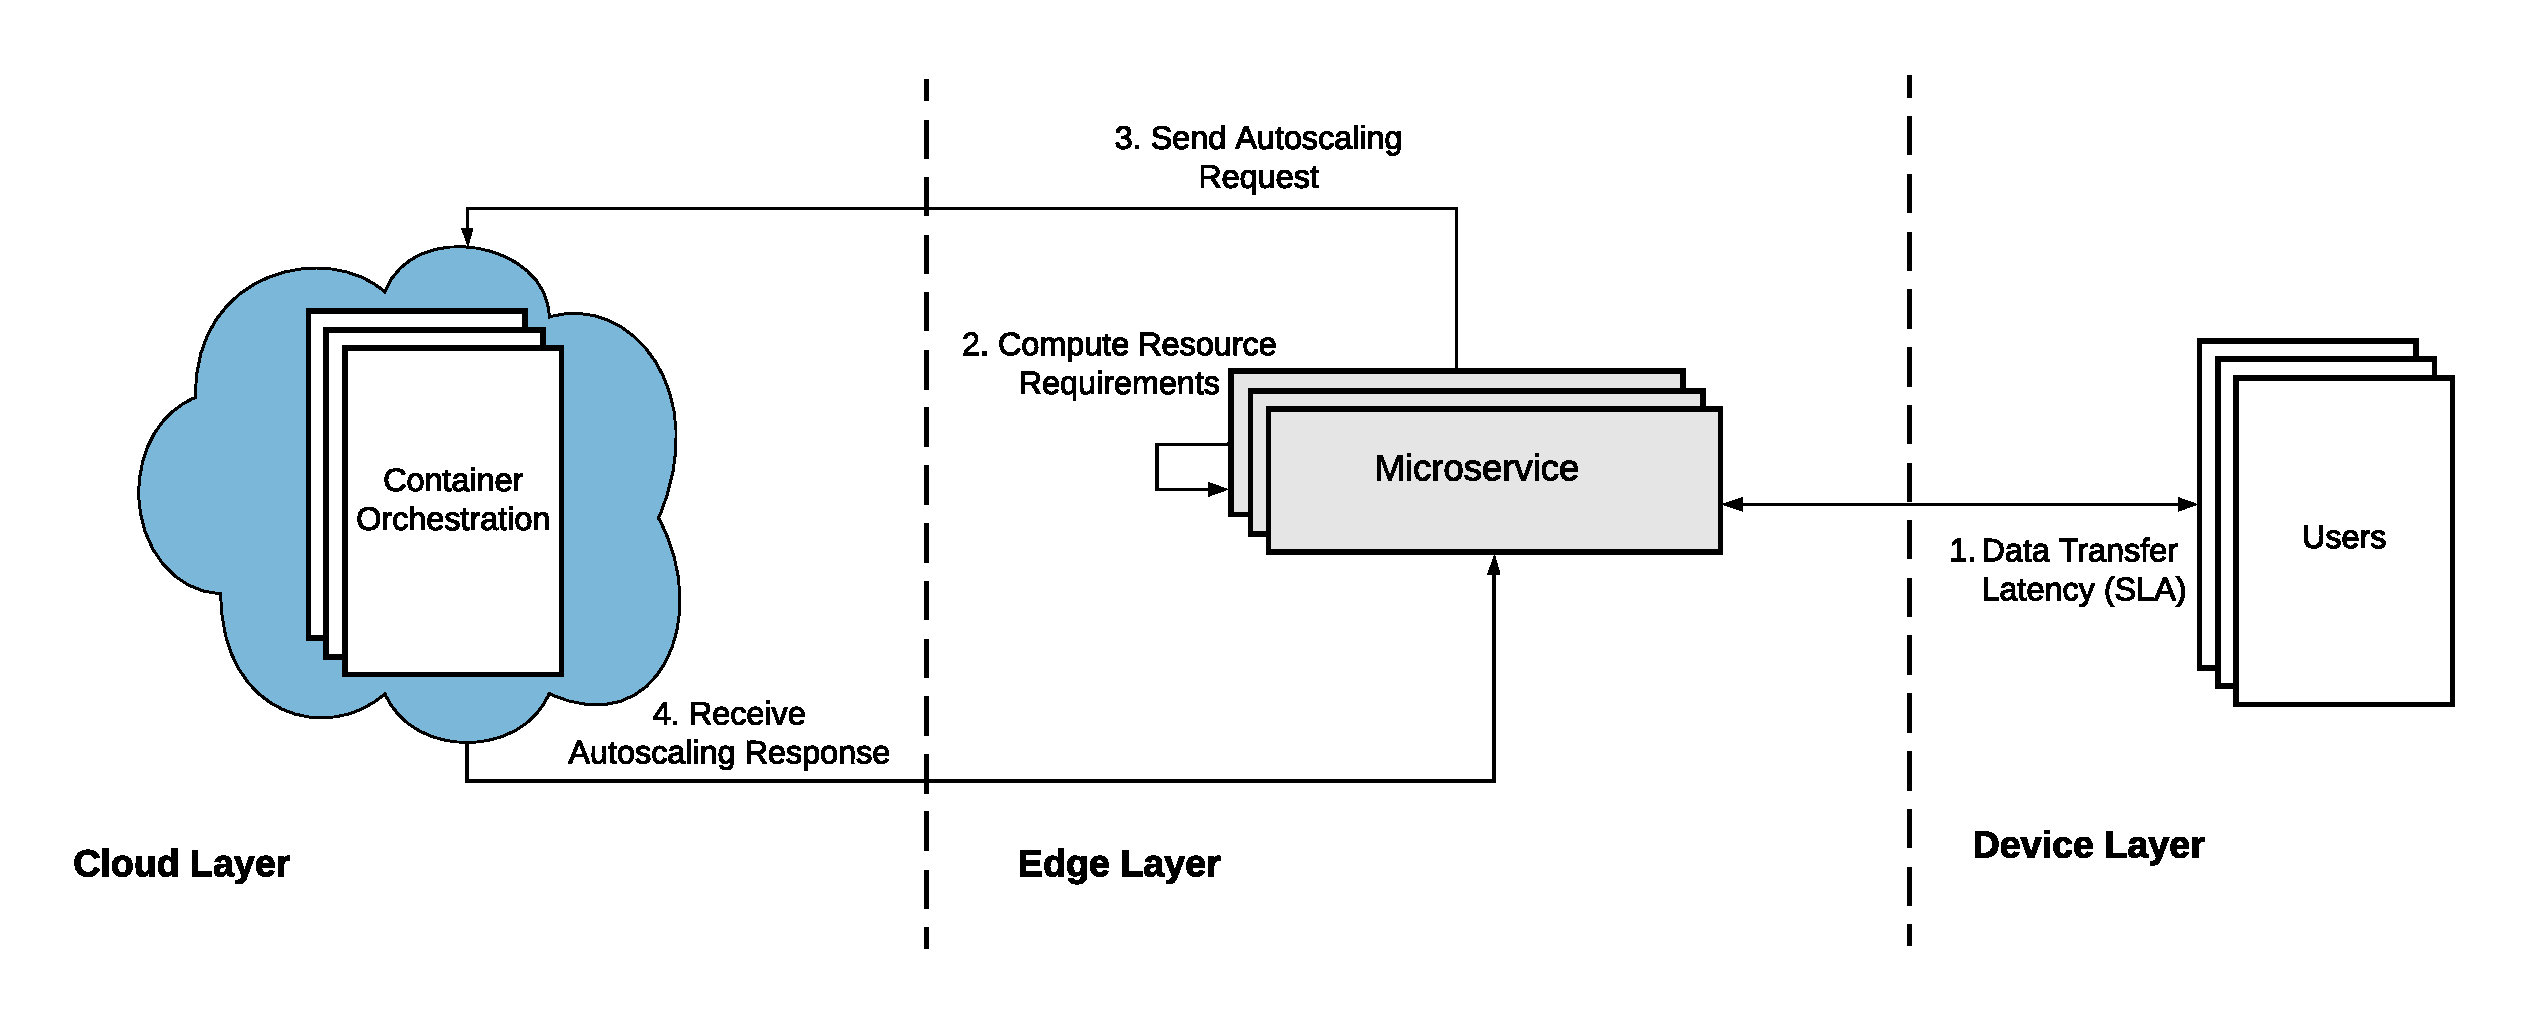
\includegraphics[width=1.0\linewidth]{Figures/Problem-Overview.pdf}
    \label{fig:autoscaling-problem-overview}
\end{figure}

The cloud layer has the most amount of resources allocated to it, which it requires when managing the entire network, computing the intensive processing of large-scale data, and coordinating the resource allocation of the edge layer. However, the primary drawback is the distance between the user and the cloud layer which results in significant latency, making it unsuitable for serving real-time user requests. Thus only system-critical applications such as the controller orchestration control plane are deployed on this layer. The edge layer has far fewer resources than the cloud layer, but its proximity to the users results in lower network latency, making it ideal for resource scaling. For this reason, the edge layer consists of the orchestration tool's worker nodes and the micro-service which receives and serves user data. These worker nodes allocate resources to the micro-service deployments dynamically according to user requirements through the process known as auto-scaling.\par

Figure~\ref{fig:autoscaling-problem-overview} shows the auto-scaling process. The users in the device layer send requests and receive responses to the micro-service deployment in the edge layer. The time taken to receive this response is considered to be the SLA latency metric negotiated between the edge deployment provider and the customer. Using the number of requests being received by the user layer, the edge layer micro-service autoscaler computes the total resource requirements to serve the customer. Based on its findings, the edge layer requests the container orchestration in the cloud layer to either downscale or upscale its resources. The container orchestration then computes the required resource allocation as well as the nodes on which to allocate them and sends its response back to the edge layer.\par

\subsection{Problem Formulation}
\label{subsec:ch4-problem-formulation}

%TC:ignore
\begin{table}
    \caption{Definition of Symbols}\label{tab:symbol-definitions}
    \centering
    \begin{tabular}{rl}
        \toprule
        \textbf{Symbol} & \multicolumn{1}{c}{\textbf{Definition}}\\
        \midrule
        $\mathcal{S}_{c}(t)$ & SLA constraint metric value at time $t$\\
        $\Delta$ & Max SLA metric threshold agreed by the cloud provider \& customer\\
        $\mathcal{V}$ & Number of SLA violations for the chosen metric\\
        $\mathcal{C}_{t}$ & ``Cold start'' time taken to scale resource replicas\\
        $req_{RT}(t)$ & Round trip latency of user request to edge layer\\
        $\mathcal{K}_{t}$ & Constant latency present between edge and device layers\\
        $\mathcal{U}(t)$ & Latency of deployment with unitary resource replica\\
        $\mathcal{D}$ & Total resources in micro-service deployment\\
        $p_{i}$ & Resource pod $i$ of deployment $\mathcal{D}$ where $i = \{1, 2, .. N\}$\\
        $\alpha$ & Cost per unit resource for cloud provider\\
        $\mathcal{L}$ & Maximum allowed deployment cost assigned by the user\\
        $\mathcal{R}(t)$ & Time taken to scale replica resources\\
        \toprule
    \end{tabular}
\end{table}
%TC:endignore

Cloud deployments provide several Quality of Service (QoS) metrics when considering SLA negotiations~\cite{serrano2016sla}. These can be broadly classified into the following four categories:

\begin{itemize}
    \item \textbf{Performance}: These are metrics such as the \textit{response time} which computes the total time taken for a user request to be processed, or the \textit{throughput}, which shows the cloud scalability.
    \item \textbf{Availability}: These include the \textit{abandon rate} which shows the ratio of dropped service requests to the total user requests, and the \textit{use rate} which calculates the amount of time a cloud service was used. Furthermore, certain performance metrics such as \textit{response time} exceeding their thresholds can be considered availability metrics as well.
    \item \textbf{Reliability}: This includes metrics such as the \textit{mean failure time} which calculates the predicted time between service failures, and the \textit{mean recovery time} which is the average time it takes for the service to recover from said failure.
    \item \textbf{Cost}: This includes \textit{financial} costs of deploying or using a cloud service, as well as \textit{energy} costs which compute the carbon footprint of running a cloud service.
\end{itemize}

For this research, we utilize the performance metric \textit{response time} of the user requests as the SLA constraint metric. This metric was chosen due to it being affected the most by intelligently auto-scaling cloud services. Reliability and cost metrics such as \textit{energy} do not correlate well to auto-scaling, while availability metrics such as \textit{abandon rate} are too vague in their reading, showing a binary value of the request either being dropped, or processed. By using this metric, the cloud deployment guaranteed that all requests would be served under a certain threshold.

For real-time applications, the auto-scaling should adhere to the SLA metric as much as possible, and try to minimize the number of violations. An SLA constraint $\mathcal{S}_{c}(t)$ is defined as a metric value not exceeding above a threshold $\Delta$ agreed by both the cloud provider and the customer.

\begin{equation}
    \mathcal{S}_{c}(t) > \Delta
    \label{eqn:sla-threshold}
\end{equation}

The threshold $\Delta$ shown in Equation~\ref{eqn:sla-threshold} varies from application to application. Hussain \textit{et al}.~\cite{hussain2016sla} provided a framework wherein multiple SLA thresholds were configured by the cloud provider and customer, so as to apply them for a variety of use cases, and to ensure differing responses based on the severity of the violation. For a response time latency based metric, these thresholds can broadly be classified into three categories.

\begin{itemize}
    \item \textbf{Flexible}: This is typically the highest allowed violation threshold for the application. Flexible SLA metrics are used to gauge the availability of the deployment. Most IoT applications employ this threshold.
    \item \textbf{Moderate}: This threshold is a trade-off between flexible and stricter SLA thresholds. This threshold is used by applications to ensure a real-time capability such as traffic light scheduling in railways.
    \item \textbf{Strict}: This is the lowest allowed violation threshold in the application. This threshold is significantly challenging to maintain and is used by extremely time-critical applications such as remote-controlled tools for medical surgeries.
\end{itemize}

The auto-scaling will thus use a resource metric to scale its resources up or down. The autoscaler will check to see if the micro-service metric exceeds the threshold for a certain time period, and if so, autoscale resources accordingly. A problem arises in the time it takes to scale these resources, however. This time to increase the number of resource replicas $\mathcal{R}$, which we define as the cold start time $\mathcal{C}(t)$ which can be defined as:

\begin{equation}
    \mathcal{C}(t) = \mathcal{R}_{download}(t) + \mathcal{R}_{deploy}(t) + \mathcal{R}_{register}(t)
\end{equation}

Here, the cold start time $\mathcal{C}(t)$ is defined as the summation of the time taken for the replica $\mathcal{R}$ to be downloaded, deployed on the data plane, and registered with the control plane for scheduling and accepting user requests. The replica image is typically downloaded from a public repository. This download time is usually a one-time delay due to optimizations done on modern container orchestration software, and can be ignored for SLA latency calculations. Using this information, we can reduce this equation to the following:

\begin{equation}
    \mathcal{C}(t) \approx \mathcal{R}_{deploy}(t) + \mathcal{R}_{register}(t)
\end{equation}


Here, the time to deploy and register the replica to the container orchestration cloud layer cannot be avoided. Furthermore, it can be shown that the number of SLA violations $\mathcal{V} \propto \mathcal{C}(t)$ due to the correlation between cold-start delay and the lack of available resources~\cite{patel2021systematic}.\par

Thus, when computing the SLA constraint value for a latency metric, the SLA latency can be re-written as the sum of the cold-start time and the round-trip time taken for the request.

\begin{equation}
    \mathcal{S}_{c}(t) = \mathcal{C}(t) + req_{RT}(t)
\end{equation}


This round-trip time $req_{RT}(t)$ is the combined sum of the inherent delay present in the network layer $latency_{N/W}(t)$, and the time taken for the edge application to process the request $processing_{app}(t)$.

\begin{equation}
    req_{RT}(t) = 2 \times latency_{N/W}(t) + processing_{app}(t)
\end{equation}

The network delay can be reduced by investing in higher network bandwidths, but such improvements have a maximum physical limit, which would not solve the cold start issue. Here we consider this latency to be a constant $\mathcal{K}(t)$. Furthermore, $processing_{app}(t)$ is inversely proportional to the available resources to the application $\mathcal{D}$, since increasing the number of resource replicas helps spread out the user request workload thus reducing the chances of a bottleneck. Using this information, $req_{RT}(t)$ can be approximated as:

\begin{equation}
    req_{RT}(t) \approx \mathcal{K}(t) + \cfrac{\mathcal{U}(t)}{\mathcal{D}}
\end{equation}

Where $\mathcal{U}(t)$ is the maximum latency of a unitary resource deployment. For horizontal pod auto-scaling, the resources here are the number of pods in deployment resources $\mathcal{D}$ such that $\mathcal{D} = \sum_{i} p_{i}$, where $i$ represents the current number of active pods. These pods are the smallest unit of resource for auto-scaling purposes that process the user requests. The final SLA equation can be re-written as follows:

\begin{equation}
    \mathcal{S}_{c}(t) = \mathcal{C}(t) + \cfrac{\mathcal{U}(t)}{\sum_{i} p_{i}} + \mathcal{K}(t)
    \label{eqn:sla-cold-start}
\end{equation}

Thus, the primary aim of the autoscaler is to significantly reduce or even eliminate the cold start, while also increasing the number of resources assigned to the deployment to minimize the application latency. By doing so, the autoscaler aims to reduce the SLA latency below the agreed threshold $\Delta$ thus minimizing the number of SLA violations $\mathcal{V}$.\par

From the above equation, it is clear that $\lim_{\sum_{i} p_{i} \to \infty} \cfrac{\mathcal{U}(t)}{\sum_{i} p_{i}} = 0$.

%\tawfiq{you may use the following to make the above argument more fancy :)}
%$\lim_{\sum_{i} p_{i} \to \infty} \frac{\mathcal{U}(t)}{\sum_{i} p_{i}} = 0$

Thus, the equation incentivizes ignoring intelligently auto-scaling altogether and simply allocate the maximum number of pods to the deployment. However, there are drawbacks to doing so.\par

Most cloud providers such as Amazon Web Services and Google Cloud Platform allocate a cost for each resource assignment to the deployment. If the maximum number of pods that can be deployed is $N$, the cost is calculated as follows.

\begin{equation}
    cost = \alpha \times \sum_{i} p_{i} \quad ;\,i \le N
    \label{eqn:cost}
\end{equation}

Where $\alpha$ is the unitary resource cost which may vary depending on the cloud provider. Thus, simply scaling all resources to the maximum amount may result in substantial and infeasibly high deployment costs. Based on this additional information, the auto-scaling SLA Equation~\ref{eqn:sla-cold-start} and the cost Equation~\ref{eqn:cost} can be merged to form an optimization problem $\mathcal{P}$.

\begin{equation}
    \mathcal{P} = x \times \mathcal{S}_{c}(t) + y \times cost
    \label{eqn:optimization-problem}
\end{equation}

The objective of the autoscaler is to assign resources in a way that minimizes both the latency, as well as the cost, thus minimizing $\mathcal{P}$. The parameters $x$ and $y$ dictate how important cost and latency are relative to each other when considering auto-scaling. For this research, we will configure these values as $x = y = 0.5$, implying both are equally important. Furthermore, the customer will have a maximum ``budget'' $\mathcal{L}$ which the deployment must not exceed. Maximizing the value of the resources in $\mathcal{D}$ while limiting the cost below the threshold $\mathcal{L}$ to reduce the SLA constraint metric $\mathcal{S}_{c}$ below the agreed threshold is akin to the famous Knapsack Problem~\cite{martello1987algorithms}. This problem is proven to be NP-Hard, and as such no known algorithm can determine the best value in polynomial time as demonstrated by Kellerer \textit{et al}.~\cite{kellerer2004introduction}. However, an approximation close to this best value can be computed instead, and this can be done in polynomial time. Due to this, most autoscalers rely on a reactive rule-based or proactive machine-learning technique to compute such close approximations.\par

A problem however arises in the amount of resources it takes to train a proactive model. Not only does the training process consume a significant amount of CPU and memory resources, but it also requires a large time-series dataset. This dataset is necessary to generate a sufficient number of training windows. Without enough training windows, the model will produce erroneous results. While hybrid models help to mitigate the initial errors via the reactive auto-scaling component, the questions regarding the proactive model's resource usage remain an open issue~\cite{radhika2021review}.\par

%Another issue in proactive autoscalers is that not only does it predict increases in utilization before-hand, it also does so for the drop-off in utilization. This can lead to the edge deployment prematurely reducing its resources due to the drop-off forecast, causing several SLA violations due to low availability of resources. To offset this, several hybrid algorithms combine the readings of their reactive and proactive autoscalers, and autoscale according to the highest reading. While this approach works, such algorithms render the accurate resource drop-off predictions of the forecaster redundant, merely taking up precious computation space in the edge deployment.\par

Another issue in a purely proactive autoscaler is the amount of time it takes to both train the model, as well as generate the predictions. Torres \textit{et al}.~\cite{torres2021deep} have demonstrated that time-series forecasters such as LSTM and ARIMA are known to typically have incredibly complex deep neural networks with thousands of neurons in several layers. They demonstrated that even when running such a deep neural network on a cloud architecture, with the aid of 6 cores of CPU and 16 GB of memory resources, and additional parallelization through the use of modern graphical processing units (GPU), this can result in the training process taking upwards of an hour. A large training time makes it incredibly difficult to actively tune the hyper-parameters of the model based on the perceived accuracy, as adapting these values too frequently would result in several hours of training per day, during which the model is unable to predict new values. Once again, a hybrid architecture is typically used to mitigate this issue, as when the proactive model is training, the reactive autoscaler takes over. However, this approach is not feasible for an SLA-constrained architecture, as the reactive component is not SLA-compliant due to its inability to mitigate the cold start problem.\par


In most proactive autoscalers, the forecaster attempts to accurately model the time-series curve to allocate resources effectively. Even in the hybrid algorithms that have been proposed in Section~\ref{sec:ch3-hybrid-solutions}, the proactive modules of the autoscalers are generally unmodified proactive forecasters bundled together with a reactive component. This strategy of attempting to perfectly forecast the curve is what takes such large amounts of resources.\par

Hence, the autoscaler proposed in this thesis will not attempt to predict the exact resource workload. Instead, the time-series graph is heavily simplified using a noise filtering method and then inputted to the machine learning model. Furthermore, the time-series forecaster only attempts to predict the exact timestamp when resource requirements start to increase. Every other requirement, such as the stable resource utilization, as well as the drop-off in non-peak time periods can be handled by the reactive autoscaler, thus heavily simplifying the forecaster architecture. This drastically reduces the forecaster training time to a few minutes. The simplified forecaster has the additional benefit of not requiring incredibly lengthy amounts of time-series data to be stored for it to make accurate predictions, thus this data can also be kept in the edge layer. This makes the autoscaler extremely lightweight, responsive, and most importantly SLA-compliant, thus making it capable of being deployed in an edge environment.\par

\section{Proposed Hybrid Autoscaler}
\label{sec:ch4-hybrid-autoscale-overview} 

\begin{figure}[htb]
    \centering
    \caption{Proposed hybrid architecture overview}
    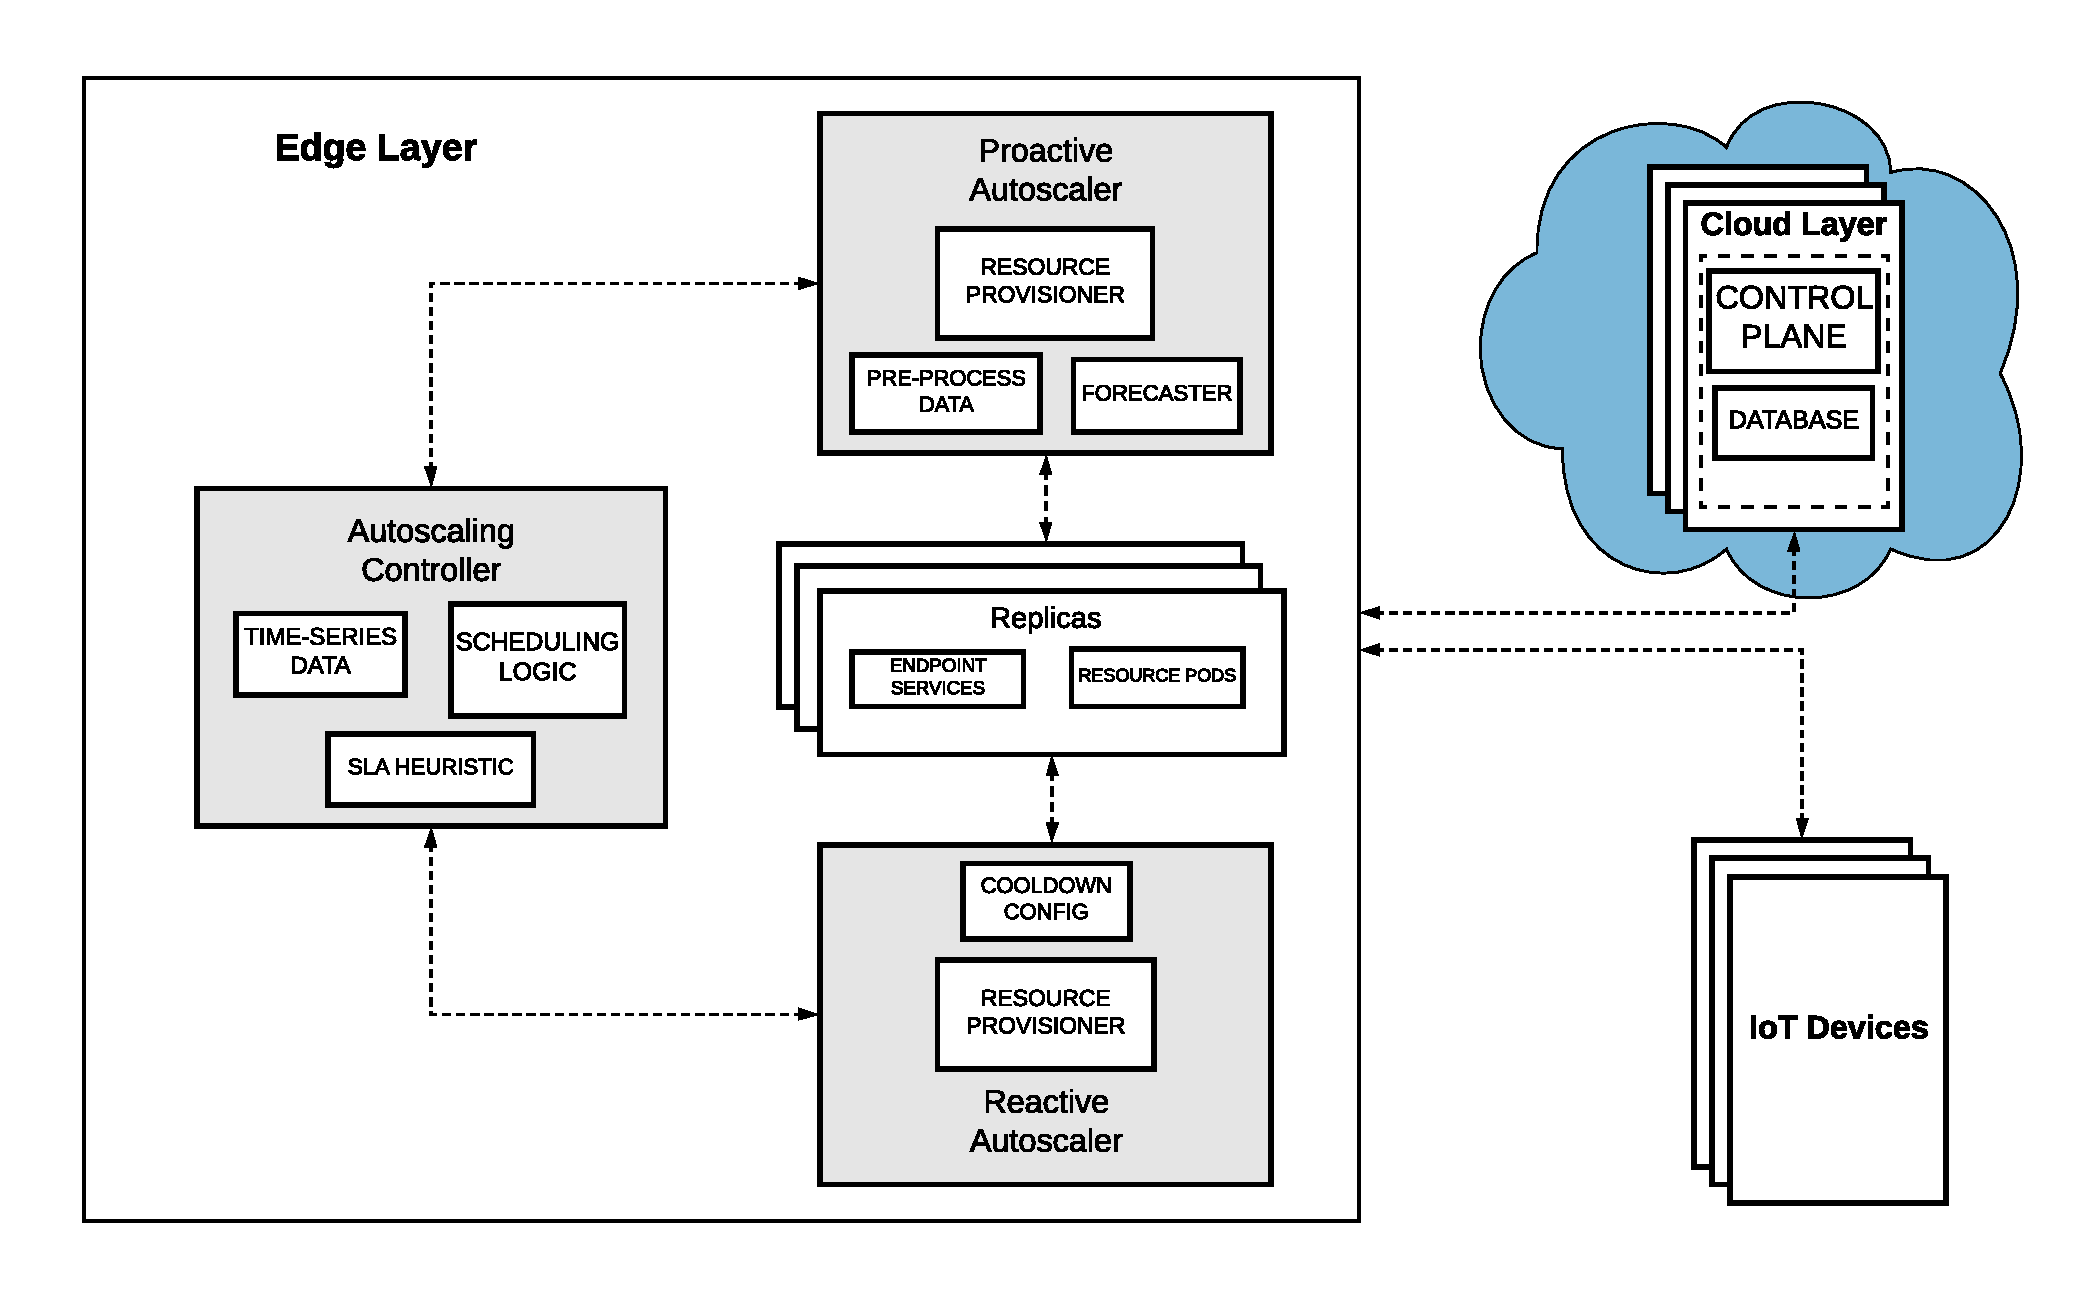
\includegraphics[width=1.0\linewidth]{Figures/Hybrid-Architecture-Overview.pdf}
    \label{fig:hybrid-arch-overview}
\end{figure}

An overview of the hybrid autoscaler architecture is shown in Figure~\ref{fig:hybrid-arch-overview}. The overall architecture is formulated using a hierarchical model as described in Section~\ref{sec:ch3-edge-implementation}. The edge node consists of three main sections. The first is the reactive auto-scaling subsystem, which has the resource provisioning module, and the configuration which dictates the cooldown logic for scaling up and down. As Zhang \textit{et al}.~\cite{zhang2019quantifying} demonstrated, the micro-service system stability is directly related to the careful selection of cool-down parameters. Thus, these must be available to the user in a configuration setting.\par

The second subsystem is the proactive autoscaler. From a high-level perspective, there are three main components. The resource provisioning module is similar to that of the reactive autoscaler, however, it also consists of a forecaster using a deep-learning-based machine learning model, and a data pre-processing algorithm. The data pre-processing algorithm removes any noise present in the time series data, and smoothens the data curves, making it easier for the forecaster to make predictions in a low-cost manner. A detailed implementation of the forecaster logic itself will be discussed in Section~\ref{subsec:ch5-proactive-auto-subsection}.\par

Finally, the auto-scaling controller determines which auto-scaling logic will be applied to the replicas, and also keeps track of any SLA violations. It also hosts the time-series metric data and has a feedback loop with the proactive autoscaler. If it detects any SLA violations were caused after auto-scaling during a configured time window, it automatically adjusts the hyper-parameters of the proactive forecaster in an attempt to predict from the time-series data more accurately during the next training iteration. Correspondingly, a lack of SLA violations during a specific time window period reverts the autoscaler parameters back to the original values, in an attempt to streamline the training process further. Such a heuristic method allows for the freeing up of the complex hyper-parameter tuning process seen in most proactive models from the autoscaler deployment process. This is a key part of the architecture which is essential in answering the research questions outlined in the thesis.\par


\subsection{Autoscaler Subsystems}
\label{subsec:ch4-hybrid-arch}

At a high level, a container orchestration's default horizontal pod autoscaler operates on the ratio between the current and desired metric values, which can be written as:

\begin{equation}
    replicas_{desired} = \lceil replicas_{current} \times \cfrac{metric_{current}}{metric_{desired}}\rceil
    \label{eqn:replica-desired}
\end{equation}

For example, for a given deployment with a current replica count as 1, if the desired metric value is 50 resource units, and the current value is 100, then the number of desired replicas will be $\lceil 1 \times \cfrac{100}{50}\rceil = 2$. There are three other important parameters that are key to controlling the process of horizontal pod scaling, namely ``tolerance'', ``scale up cooldown'', and ``scaledown cooldown''.\par

The tolerance is a constant which informs the autoscaler when to skip calculating new replicas. The tolerance ratio can be calculated as:

\begin{equation}
    \label{eqn:tolerance}
    tolerance = \abs{ \cfrac{metric_{desired} - metric_{current}}{metric_{desired}} }
\end{equation}

For example, if the current metric is 60, and the desired metric is 50, the tolerance is calculated as $ tolerance = \abs{ \cfrac{60 - 50}{60}} = 0.167$. By default, if the tolerance value is below 0.1, autoscaling is skipped for that control loop, however, this can be configured by the user.\par

The scale-up and scale-down cooldowns control how quickly auto-scaling occurs. The default approach which is set by the container orchestration can be concisely stated as ``Scale up as quickly as possible, while scaling down very gradually.'' Therefore, the default scale-up cooldown is set to 0 seconds, meaning that the moment the desired replica value increases, the autoscaling will be initiated. However, the default cooldown is set to 300 seconds, meaning that if the desired replica value is decreased, it must remain decreased for 300 seconds (or 20 control loops) before the resources are scaled down.\par

A cooldown value that is too low would cause a repetitive scaling up and scaling down of the resources, leading to significant stress on the system as well as wastage of resources. Meanwhile, a large value would render the autoscaler unable to assign resources quickly enough to ensure SLA latency compliance. Thus, for the proposed autoscaler, the default values are modified to ensure that a moderate cooldown value was chosen to ensure the best system stability and SLA compliance. This cooldown configuration would be applied to both the proactive and reactive auto-scaling subsystems to maintain consistency.\par

For auto-scaling proactively, a custom metric $metric_{forecast}$ is used, which defines the future CPU workload expected to be exerted on the micro-service application $\mathcal{T}$ seconds in the future, where $\mathcal{T}$ can be configured during the autoscaler deployment process. This $metric_{forecast}$ value will be sent to the auto-scaling controller by the proactive autoscaler.\par

\subsubsection{Scheduler}

The autoscaler controller consists of a scheduling logic module which handles when to switch between proactive and reactive auto-scaling. Algorithm~\ref{alg:scheduling-logic-daemon} explains how the hybrid scheduling logic determines which auto-scaling subsystem to employ. The hybrid scheduler takes four inputs, namely the $replicas_{current}$, $metric_{current}$, $metric_{desired}$, and $metric_{forecast}$ variables discussed above. It outputs one value, the $replicas_{desired}$.\par

The autoscaler computes two replica values, one for the proactive forecaster which determines the replicas after $\mathcal{T}$ seconds, and one for the reactive forecaster, which determines the current resource requirements. By computing the future requirements $replicas_{forecast}$ using Equation~\ref{eqn:replica-desired}, if it is found that this requirement is higher than the current resource requirement $replicas_{current}$, then the hybrid scheduler outputs the forecaster replica count as the desired replicas. Otherwise, the hybrid scheduler determines that the utilization is either stabilizing or about to decline. Due to this, it makes a decision that the reactive replica count $replicas_{reactive}$ is the desired number. The hybrid scheduler then sends this value to the container orchestration controller plane to autoscale the replicas accordingly using either the reactive or proactive sub-system's resource provisioning modules.\par

%TC:ignore
\begin{algorithm}
    \caption{Scheduler algorithm}
    \label{alg:scheduling-logic-daemon}
    \textbf{Input}: $replicas_{current},\, metric_{current},\, metric_{desired},\, metric_{forecast}$\\
    \textbf{Output}: $replicas_{desired}$
    \begin{algorithmic}
        \State $replicas_{forecast} \gets \lceil replicas_{current} \times \cfrac{metric_{forecast}}{metric_{desired}}\rceil$
        \State $replicas_{reactive} \gets \lceil replicas_{current} \times \cfrac{metric_{current}}{metric_{desired}}\rceil$
        \If{$replicas_{forecast} > replicas_{reactive}$}
            \State $replicas_{desired} \gets replicas_{forecast}$
        \Else
            \State $replicas_{desired} \gets replicas_{reactive}$
        \EndIf
        \State \Return $replicas_{desired}$
    \end{algorithmic}
\end{algorithm}
%TC:endignore

\subsubsection{Reactive Resource Provisioning}

The reactive autoscaler subsystem is responsible for determining whether or not auto-scaling should proceed based on the given configuration. The reactive algorithm's resource provisioning is built on top of the default horizontal pod autoscaler deployed by the Kubernetes container orchestration platform. The autoscaler is modified in such a way that it has its cooldown parameters set to a moderate value to ensure adaptability to SLA-constrained scenarios, while also maintaining system stability. The workflow is shown below in Algorithm~\ref{alg:reactive-resource-provision}. The algorithm takes the current metric value as an input, as well as the desired metric value, and outputs the decision to autoscale or not. It does this by computing the $tolerance$ value as shown in Equation~\ref{eqn:tolerance}. If this tolerance is above the configured threshold, the autoscaler will modify the replicas, otherwise, it will ignore the current auto-scaling request.\par

%TC:ignore
\begin{algorithm}
    \caption{Reactive resource provisioning}
    \label{alg:reactive-resource-provision}
    \textbf{Input}: $metric_{current},\, metric_{desired}$\\
    \textbf{Output}: $autoscale$
    \begin{algorithmic}
        \State $tolerance \gets \abs{ \cfrac{metric_{desired} - metric_{current}}{metric_{desired}} }$
        \If{$tolerance > \gamma$}
            \State $autoscale \gets Yes$
        \Else
            \State $autoscale \gets No$
        \EndIf
        \State \Return $autoscale$
    \end{algorithmic}
\end{algorithm}
%TC:endignore

\subsubsection{Data Pre-Processor}
\label{subsubsec:ch4-data-pre-process}

\begin{figure}[htb]
    \centering
    \caption[Pre-processing of data]{Pre-processing of data, source:~\cite{comsolcurvefitting}}
    \label{fig:data-pre-process}
    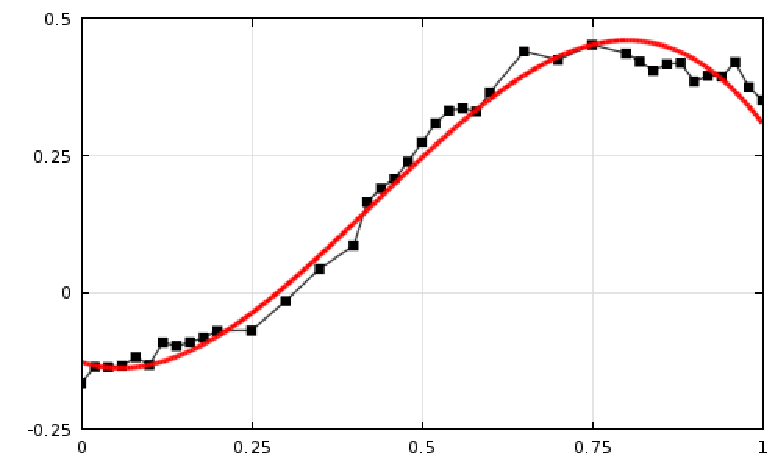
\includegraphics[width=0.6\linewidth]{Figures/Data-Pre-Processing.pdf}
\end{figure}

To speed up the forecast process even further and reduce the resource and time requirements, the time-series data can be pre-processed to smoothen it. Doing so makes it easier for the deep learning model to extract patterns, and reduces the training and validation loss. Figure~\ref{fig:data-pre-process} shows a graph containing raw input (shown in black), and a smoothened data curve (shown in red). While the red curve contains all the requisite information of the data (such as the slope of the curve, maximum and minimum value, etc.), it removes the noise, reducing the overall loss, and reducing the length of the training window data sequence the LSTM requires to accurately predict future data.\par

\subsubsection{Proactive Forecaster}

The forecaster portion of the autoscaler is used to generate this $metric_{forecast}$ value. The autoscaler controller periodically scrapes the windowed data stored in the cloud database to keep a form of cached time-series workload. It combines this workload with the future workload $metric_{forecast}$. To do so, the controller requests the $metric_{forecast}$ value for a specified time $\mathcal{T}$ from the proactive forecaster, and the forecaster then sends this value back after pre-processing the scraped data and training the forecaster model.\par

Several time series forecaster algorithms exist, with the two prominent ones being the more modern deep learning algorithm LSTM, and the traditional deep learning algorithm ARIMA. Siami-Namini \textit{et al}.~\cite{siami2018comparison} demonstrated that LSTM implementations outperformed ARIMA, reducing error rates by over 80\%. Furthermore, they were able to demonstrate that the number of deep learning ``epochs'', or the total amount of training time required for LSTM did not need to be set to a high value. In fact, setting a significantly higher value than required was shown to degrade performance due to over-fitting. The authors posited that LSTM worked so well due to the ``rolling updates'' being performed on the model. The LSTM weights are only set once when the forecaster is deployed, after which they are always updated on every call of the training algorithm, meaning there is a continuous improvement to the prediction results.\par

Based on the investigations above, it was determined that LSTM time-series forecasters would be ideally suited for a proactive autoscaler designed for the hybrid autoscaler architecture. Algorithm~\ref{alg:proactive-forecast-alg} shows the implementation of such a forecaster. The autoscaler controller implements a control loop every $\mathcal{P}$ seconds, where it requests the latest time-series metric prediction from the forecaster. As input, the algorithm takes the variable $lookback$, which is the number of data points it should use as a window to train, the training iteration count $epochs$, and the $learning\_rate$, which determines the step size per each training iteration moving towards the minimum loss value. The forecaster then pre-processes this data to remove the noise as shown above in Section~\ref{subsubsec:ch4-data-pre-process}, and performs a training iteration using the configured hyper-parameters. It then computes the validation loss, and accepts this model as the most accurate one if it has a lower validation loss than the previous training iterations. Otherwise, the current model is rejected and the forecaster uses the older model instead. Finally, the model predicts the future metric and returns it to the autoscaler controller for determining the auto-scaling based on Algorithm~\ref{alg:scheduling-logic-daemon}.\par


\begin{algorithm}
    \caption{Proactive forecaster}
    \label{alg:proactive-forecast-alg}
    \textbf{Input}: $lookback \geq 0, 0 \leq epochs \leq 100, 0 \leq learning\_rate \leq 1$\\
    \textbf{Output}: $metric_{forecast}$
    \begin{algorithmic}
        \State $lstm\_model \gets lstm.initialize()$
        \State $time\_series \gets get\_latest\_data()$
        \State $lstm\_input \gets get\_input(time\_series\_data, lookback)$
        \State $lstm\_input \gets preprocess\_data(lstm\_input)$
        \State $new\_model \gets train(lstm\_input, epochs, learning\_rate)$
        \If{$validation\_loss(new\_model) < validation\_loss(lstm\_model)$}
            \State $lstm\_model \gets new\_model$
        \EndIf
        \State $metric_{forecast} \gets lstm\_model.predict(lstm\_input)$
        \State \Return $metric_{forecast}$
    \end{algorithmic}
\end{algorithm}

\subsubsection{Proactive Resource Provisioning}

The proactive subsystem's resource provisioning module works in a similar manner to the reactive autoscaler. If the autoscaler controller's scheduling logic determines that a proactive auto-scaling must take place, it requests the cloud layer to proceed with auto-scaling using the proactive subsystem's resource provisioning, which is shown in Algorithm~\ref{alg:proactive-resource-provision}. The algorithm takes the desired and forecast metric values as input and outputs the decision to autoscale or not. It does this by computing the $tolerance$ value as shown in Equation~\ref{eqn:tolerance}. If this tolerance is above the configured threshold, the autoscaler will modify the replicas, otherwise, it will ignore the current auto-scaling request.\par

\begin{algorithm}
    \caption{Proactive resource provisioning}
    \label{alg:proactive-resource-provision}
    \textbf{Input}: $metric_{forecast},\, metric_{desired}$\\
    \textbf{Output}: $autoscale$
    \begin{algorithmic}
        \State $tolerance \gets \abs{ \cfrac{metric_{desired} - metric_{forecast}}{metric_{desired}} }$
        \If{$tolerance > \gamma$}
            \State $autoscale \gets Yes$
        \Else
            \State $autoscale \gets No$
        \EndIf
        \State \Return $autoscale$
    \end{algorithmic}
\end{algorithm}

\subsubsection{SLA Heuristic Feedback}

Finally, the last hybrid autoscaler module is the autoscaler controller's SLA-based heuristic feedback loop, which assists the proactive forecaster in increasing its prediction accuracy. The autoscaler constantly checks for SLA violations in the edge deployment using a control loop. Typically, the SLA checks are done for a sufficiently lengthy period of time such as one day. If an SLA violation is found, it is concluded that the application was unable to autoscale quickly enough to avoid the cold start problem. This could be due to a number of causes, such as insufficient training data, or the LSTM hyper-parameters being too conservative. To temporarily boost learning, the controller then decreases the learning rate to increase the probability of the model escaping from the local minima to find the global one, increases the batch size to reduce under-fitting, and increases the number of epochs to reduce loss. All these parameters have a threshold, as increasing or decreasing certain parameters by a large amount may lead to issues such as over-fitting or infeasibly lengthy training times.\par

\begin{algorithm}
    \caption{SLA-based heuristic feedback}
    \label{alg:sla-heuristic-feedback}
    \textbf{Input}: $\mathcal{V},\,learning\_rate,\,batch\_size,\,epochs$\\
    \textbf{Output}: $hyperparameters_{modified}$
    \begin{algorithmic}
        \State $initial\_rate \gets learning\_rate$
        \State $initial\_batch \gets batch\_size$
        \State $initial\_epochs \gets epochs$
        \If{$\mathcal{V}$ > 0}
            \State $batch\_size \gets MAX(batch\_size + \alpha, \mathcal{A})$
            \State $learning\_rate \gets MIN(learning\_rate - \beta, \mathcal{B})$
            \State $epochs \gets MIN(epochs - \lambda, \mathcal{L})$
        \Else
            \State $epochs \gets initial\_epochs$
            \State $learning\_rate \gets initial\_rate$
            \State $batch\_size \gets initial\_batch$
        \EndIf
        \State $hyperparameters_{modified} \gets (learning\_rate, batch\_size, epochs)$
        \State \Return $hyperparameters_{modified}$
    \end{algorithmic}
\end{algorithm}

Finally, if the feedback control loop discovers that no SLA-violations occurred during the time-period, it concludes that the LSTM has sufficiently learned the primary characteristics of the time-series. As discussed by Siami-Namini \textit{et al}.~\cite{siami2018comparison}, the ``rolling-updates'' feature of LSTM allows the autoscaler to safely reset the hyper-parameters of the model, while preserving the learning and weights of the previous rounds of training. Algorithm~\ref{alg:sla-heuristic-feedback} shows how the heuristic feedback is set up. The algorithm takes the three hyper-parameters of the LSTM, namely $learning\_rate$, $batch\_size$, and $epochs$, along with the $\mathcal{V}$ which stores the number of SLA violations that occurred during a specified time window. Using these parameters, the algorithm computes the new LSTM hyper-parameters and outputs them to the proactive forecaster to use in the next training cycle.\par

\subsection{Computational Complexity Analysis}
\label{subsec:ch4-space-time-comp}

To analyze the space and time complexity of the auto-scaling architecture, some simplifying assumptions must be made. Firstly, the complexities will be for one control loop of the container orchestration platform. By default, controller orchestration platforms have control loops which are executed every 15 seconds. During each of these loops, auto-scaling is assessed and implemented. Thus we will ignore the complexities involved in the control loop itself, and focus only on the autoscaler.\par

Secondly, for the proactive forecaster, the complexities of the LSTM are simplified to the basic multiplicative steps involved in the training step. Other internal logic such as the $\sigma$ function is assumed to have $\mathcal{O}(1)$ space and time complexity.\par

Finally, assuming the hybrid autoscaler $\mathcal{H}$ takes a time-series data of length $\mathcal{N}$, it stores this data in an array data structure. The rest of the inputs can be considered as single variables. The forecaster's LSTM weights are assumed to be a two-dimensional matrix of size $A \times B$. Thus the space complexity can be easily computed for this information. The variables each have a space complexity of $O(1)$. Meanwhile, the time-series array has a complexity of $\mathcal{O}(N)$, and the weights are of complexity $\mathcal{O}(N^2)$. Thus, the space complexity can be written as the sum of the two values and simplified.

\[Complexity_{space}(\mathcal{H}) = \mathcal{O}(N^2) + \mathcal{O}(N) + \mathcal{O}(1)\]
\begin{equation}
    \Rightarrow Complexity_{space}(\mathcal{H}) = \mathcal{O}(N^2)
\end{equation}

The time complexity is a more complex calculation. The complexities of the reactive autoscaler, proactive autoscaler, and autoscaler controller need to be computed. The autoscaler controller only stores the time-series array and computes the new hyper-parameters in Algorithm~\ref{alg:sla-heuristic-feedback}. Both of these operations can be completed in constant time, thus the time complexity for the controller is as follows:

\begin{equation}
    Complexity_{time}(controller) = \mathcal{O}(1)
\end{equation}

Similarly, the reactive autoscaler only computes the tolerance value, which is also a constant operation independent of data size, thus the time complexity can be written as:

\begin{equation}
    Complexity_{time}(reactive) = \mathcal{O}(1)
\end{equation}

For the proactive autoscaler, the forecaster internally computes matrix multiplications, such as of the various LSTM weights and vectors. For example, Equation~\ref{eqn:input-gate} can be rewritten as follows.

\begin{equation}
    i_{t} = \sigma(W_{i}(x) \cdot x_{t} + W_{i}(h) \cdot h_{t-1} + b_{i})
\end{equation}

In the above equation, we assume the dimension of the variables as follows:

\begin{itemize}
    \item $W_{i}(x) \in \R^{m \times n}$
    \item $x_{t} \in \R^{n}$
    \item $W_{i}(h) \in \R^{m \times m}$
    \item $b_{i} \in \R^{m}$
    \item $h_{t-1} \in \R^{m}$
\end{itemize}

Using these values, the time complexity of each of the individual multiplicative and additive operations can be computed.

\[Complexity_{time}(W_{i}(x) \cdot x_{t}) = \mathcal{O}(mn)\]
\[Complexity_{time}(W_{i}(h) \cdot h_{t-1}) = \mathcal{O}(m^2)\]
\begin{equation}
    Complexity_{time}(W_{i} \cdot [x_{t}, h_{t-1}] + b_{i}) = \mathcal{O}(mn + m^2 + m)
\end{equation}

Therefore the complexity of the proactive component can be written as:

\[Complexity_{time}(proactive) = \mathcal{O}(mn + m^2 + m)\]
\[\Rightarrow Complexity_{time}(proactive) = \mathcal{O}(m \times (m + n + 1))\]
\begin{equation}
    \Rightarrow Complexity_{time}(proactive) = \mathcal{O}(N^2)
\end{equation}

This is the value of one training epoch. For an LSTM training process with $\tau$ training epochs, the complexity becomes $\mathcal{O}(\tau N^2)$. However, it is important to note that the value of $\tau$ is a constant, thus the final proactive complexity can be reduced back to $\mathcal{O}(N^2)$.\par

Combining the time complexities of all three hybrid components, the final complexity for the hybrid autoscaler $\mathcal{H}$ can be re-written as:

\[Complexity_{time}(\mathcal{H}) = \mathcal{O}(1) +  \mathcal{O}(1) + \mathcal{O}(N^2)\]

\begin{equation}
    \label{eqn:hybrid-time-complexity}
    \Rightarrow Complexity_{time}(\mathcal{H}) = \mathcal{O}(N^2)
\end{equation}

From the results in Equation~\ref{eqn:hybrid-time-complexity}, it is clear that the hybrid algorithm performs extremely well in a polynomial time complexity. Even though it is shown that no mathematically certain decision can be computed in a polynomial time due to the NP-Hard nature of the problem statement, the hybrid algorithm is proven to provide an alternative that is able to approximate a high accuracy auto-scaling decision in polynomial time.
\clearpage

\def\chaptertitle{System Implementation}

\lhead{\emph{\chaptertitle}}

\chapter{\chaptertitle}
\label{ch:experimental-setup}

Based on the previous high-level overview of the architectures and algorithms involved, in this chapter we will first discuss the micro-service application architecture used to test the auto-scaling on, along with its features in Section~\ref{sec:ch5-microservice-overview}. With this background, Section~\ref{sec:ch5-data-generation} will give an explanation of the workload generator bundled along with the micro-service deployment, and how that was used to generate the time-series workload typically seen in edge deployments. Finally, we will discuss the technical configurations of the hybrid autoscaler itself in Section~\ref{sec:ch5-hybrid-auto-arch}. This will involve how the workload information is communicated between cloud and edge layers, how the autoscaler parameters for both reactive and proactive subsystems are configured, and how the forecaster is configured to use the time-series data to generate forecast values for a sufficiently large time-period to minimize training times even further. Finally, the hyper-parameter tuning configured by the autoscaler controller will be further elaborated.

\section{Micro-service Overview}
\label{sec:ch5-microservice-overview}

The container orchestration used for deploying the micro-service deployment, custom hybrid autoscaler, as well as all the additional telemtry tools was Kubernetes. Kubernetes offered the highest configurability for such a project, and combined with its ease-of-use, made it ideal for stress testing auto-scaling. DeathStarBench~\footnote{\url{https://github.com/delimitrou/DeathStarBench/tree/master/socialNetwork}}, a social network micro-service implementation developed by Y. Gan \textit{et al}.~\cite{gan2019open} was purpose-built for conducting benchmarks on edge architectures with constraints such as SLA agreements, and was thus deployed on the Kubernetes platform. The application mimics a typical large-scale social network application and supports common actions such as registering and login for user credentials, creating user posts on their timeline, reading other user timelines, receiving follower recommendations, following and unfollowing of other users, and searching for users or posts. Figure~\ref{fig:social-network-arch} shows the detailed architecture of the micro-service.\par

\begin{figure}[htb]
    \centering
    \caption[Social-Network architecture]{Social-Network architecture, source:~\cite{gan2019open}}
    \label{fig:social-network-arch}
    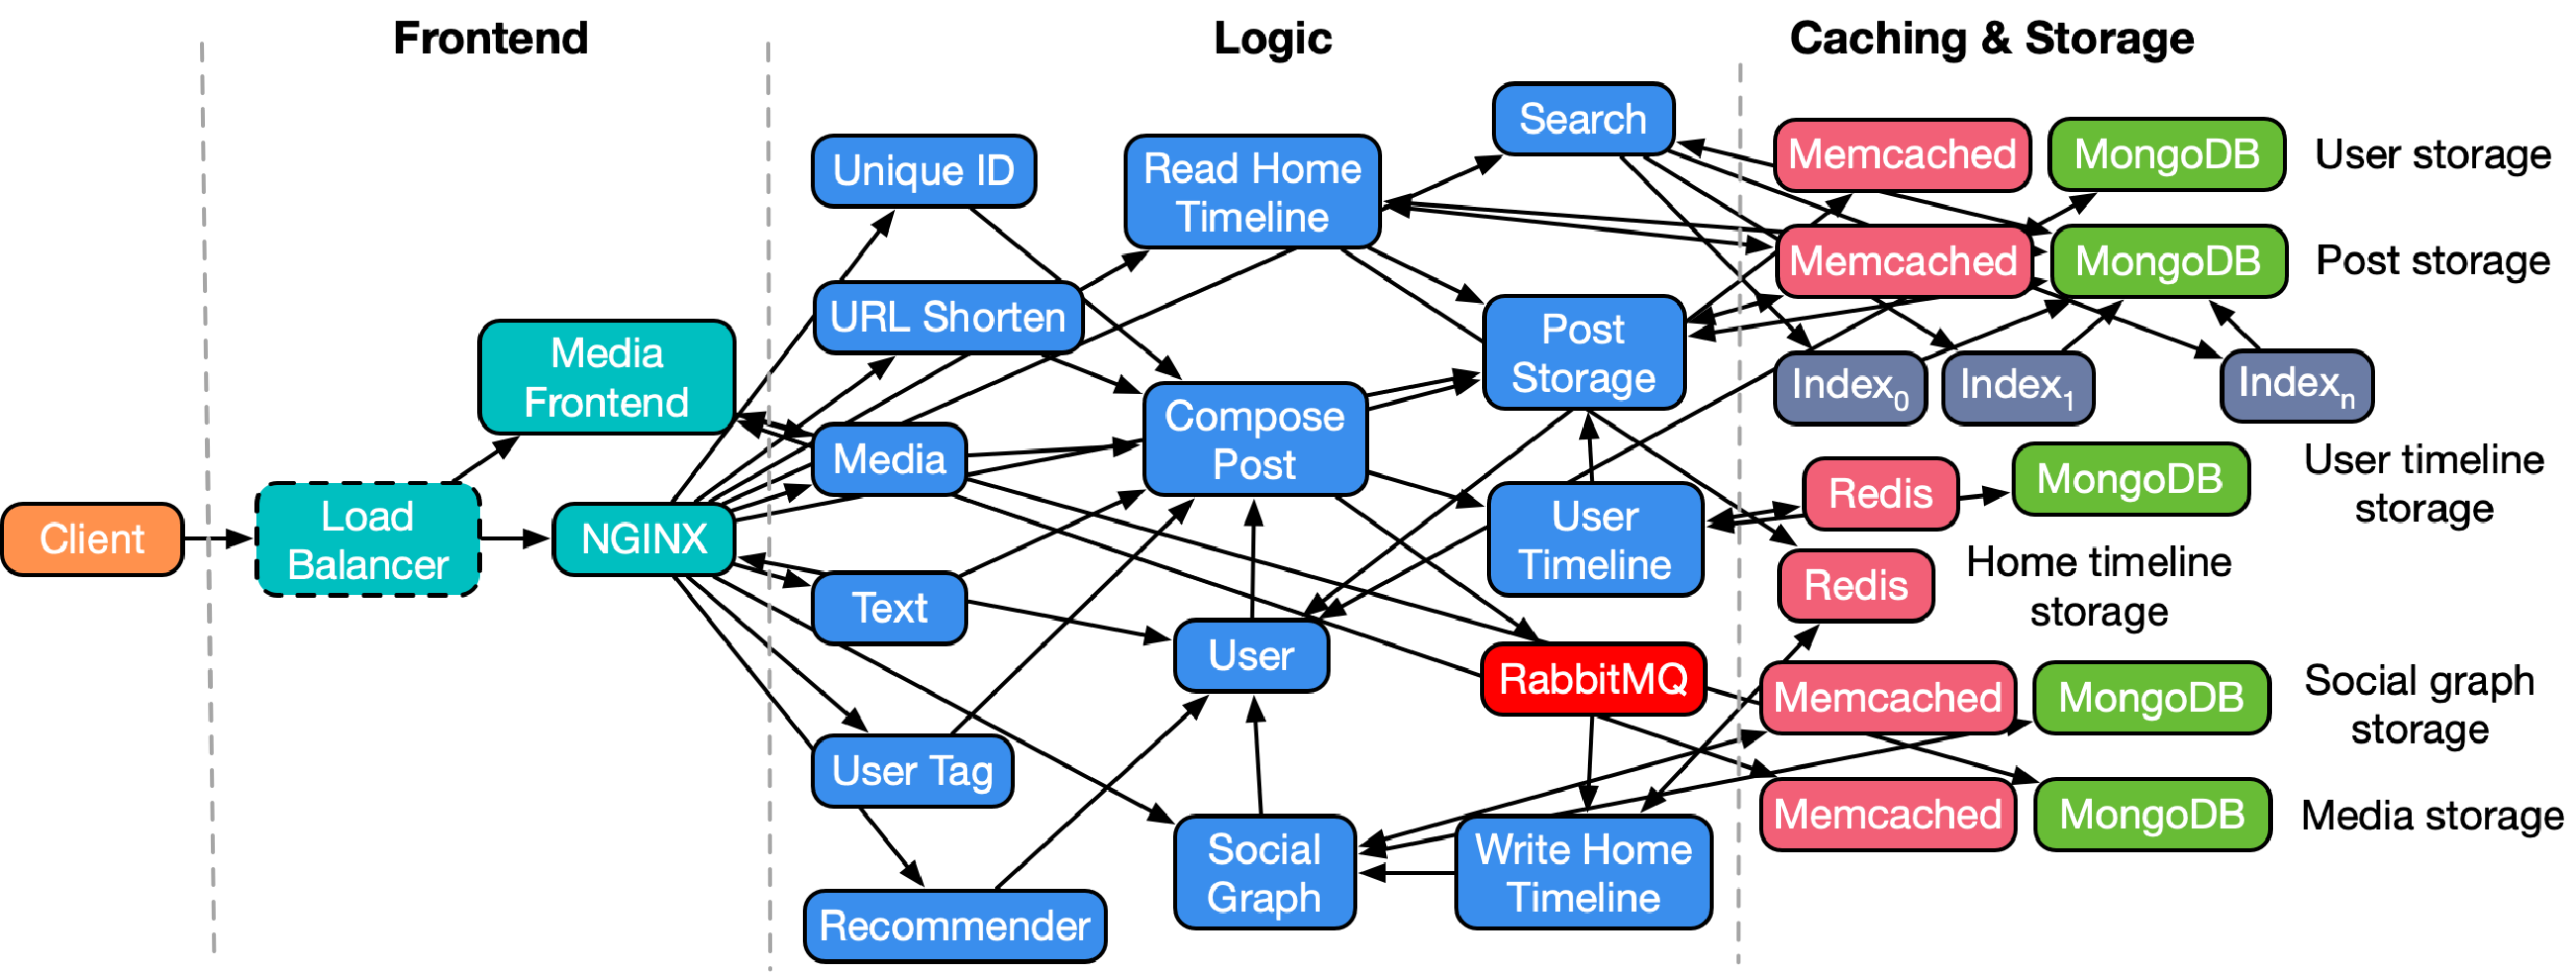
\includegraphics[width=1.0\linewidth]{Figures/Social-Network-Architecture.pdf}
\end{figure}

The end-to-end service implementation depicts a social network with a broadcast style approach. The user or client sends requests using HTTP to the front-end layer. These requests are processed using NGINX~\footnote{\url{https://nginx.org/en/}}, which is an open-source load balancer implementation. NGINX then specifies the web server that has been selected, and communicates with the micro-services in the logic layer, which are responsible for composing and displaying the user and timeline posts. The logic layer also consists of micro-services for serving advertisements, search engines, and other capabilities commonly found in large scale applications. The search and advertisement engines are machine learning plugins capable of serving recommendations based on user interactions. The logic layer is capable of handling posts containing text, links, and media. Users can also mark other user's posts as favourites, re-post them, and reply to them privately or publicly. Users can also follow, unfollow, or block others. All these interaction results are stored in the storage layer, which uses memcached for caching results, and MongoDB for storing user profiles, posts, media, and recommendations in a persistent manner.

Users can sign in to the application website by connecting to the user interface deployment, which can be assigned a DNS address. For simplicity, in this experiment the DNS configuration was skipped in favour of exposing the Kubernetes cluster IP address of the front-end deployment, along with the social media application port. For example, an API request for reading user timelines will look as follows:\par

\begin{comment}
\begin{lstlisting}[
  caption={Social network API call template},
  captionpos=t,
  label={lst:social-network-api-template},
]
http://<app-IP>:<app-port>/wrk2-api/user-timeline/read
\end{lstlisting}
\end{comment}

\texttt{http://<app-IP>:<app-port>/wrk2-api/user-timeline/read}

\section{Data Generation}
\label{sec:ch5-data-generation}

The social media deployment also comes with an HTTP workload generator, which
was leveraged to create a realistic simulation of a typical day of workload for the micro-service application. The generator, known as \textit{wrk2}, is an open-loop load generator. HTTP requests are sent out according to the user configuration, regardless of whether or not the responses of the previous requests have been received. This avoids issues such as queuing delays in the server, helping to maintain an even load throughout the generation process which aids in benchmark process. The workload generator supports a variety of load generation use-cases, as well as different APIs. For example, a POST request with a total load generation of 8 requests per second, using 2 parallel threads, with 5 open HTTP connections, and for a duration of 30 seconds looks as follows:\par

\begin{comment}
\begin{lstlisting}[
  caption={Workload generation example},
  captionpos=t,
  label={lst:workload-gen-example},
  language=bash
]
$ wrk2 -t2 -c5 -d30 -R8 http://<app-IP>:<app-port>/wrk2-api/post/compose
\end{lstlisting}
\end{comment}

\texttt{\$ wrk2 -t2 -c5 -d30 -R8 http://<app-IP>:<app-port>/wrk2-api/post/compose}

A typical IoT application in the edge has a semi-predictable workload pattern. What this means is that while the exact workloads may vary from day to day, the overall pattern of when the workloads peak and drop mostly remain constant from day to day. Tadakamalla and Menasc{\'e}~\cite{tadakamalla2019characterization} demonstrated this through a survey of three popular IoT datasets. Their results demonstrated that IoT application workloads can be well approximated using a lognormal distribution. Furthermore, the authors also observed that the daily routines of the users greatly affected the workload patterns in the dataset. This information is used to inform our own workload generation, to inject predictable patterns in the hourly data.\par

\begin{figure}[htb]
    \centering
    \caption[IoT data characteristics]{IoT data characteristics, source:~\cite{tadakamalla2019characterization}}
    \label{fig:iot-workload-characteristics}
    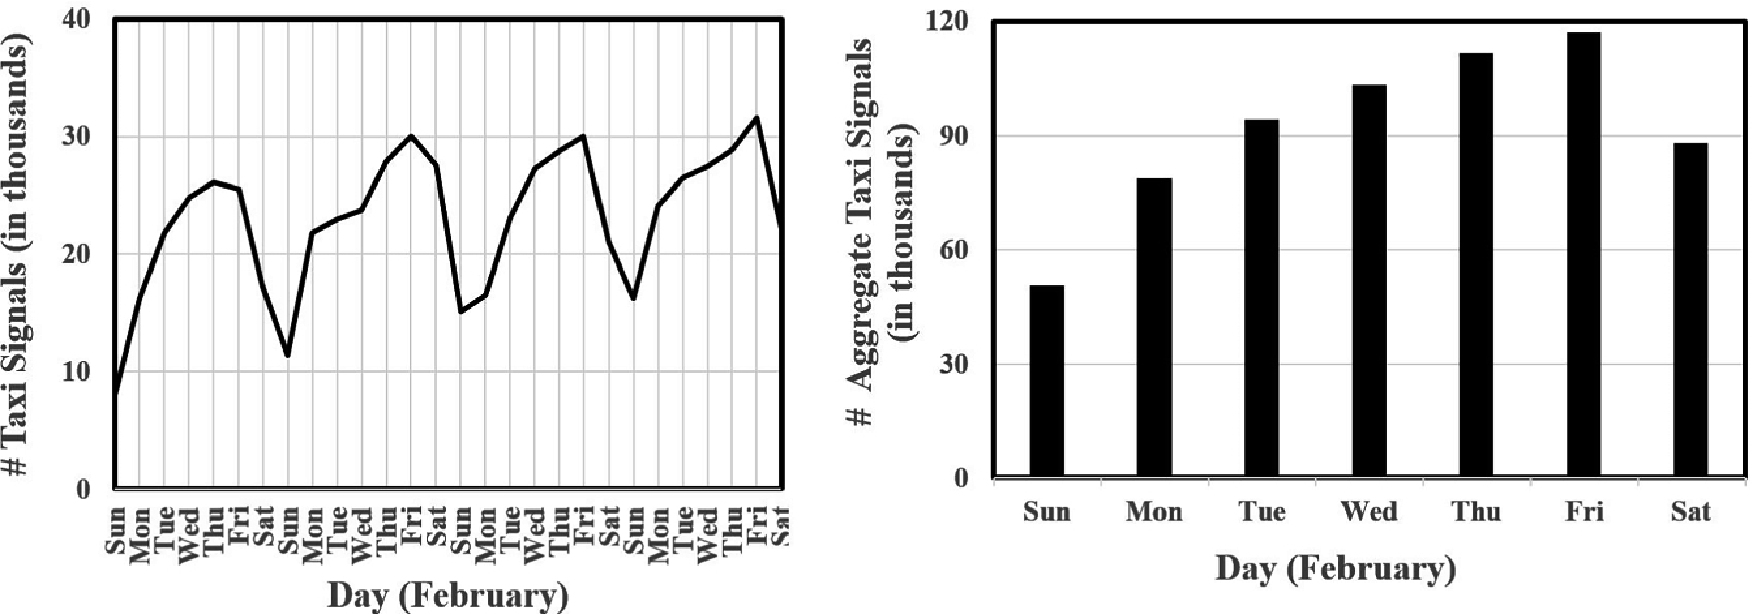
\includegraphics[width=1.0\linewidth]{Figures/IoT-Workload-Characteristics.pdf}
\end{figure}

In this experiment, it is assumed that the workload peaks in the morning and evening, while seeing moderate usage during the afternoon. The workload is lowest at night, maintaining a low usage throughout. The workload simulator was modified to introduce an element of randomness to mimic realistic weekly workloads, which can vary on occasions such as weekends and public holidays.\par

To achieve this, an IoT workload algorithm was created for leveraging the \textit{wrk2} generator to achieve this time-series. This is explained in Algorithm~\ref{alg:work-gen}. A constant light workload is set for night time consisting of six hours between 12:00am and 06:00 am, while different workloads for the rest of the 18 hours of the day are manually set, with peaks set in the morning and evening, and dips in the afternoon. The algorithm also contains a small random ``offset'' variable to depict the randomness inherent in the workload. This is depicted using the function $\mathcal{F}$, where $\mathcal{F}(0,1)$ returns a random number between 0 and 1. This workload is then executed using the \textit{wrk2} generator to apply the HTTP load on the micro-service.

\begin{algorithm}
    \caption{IoT daily workload generation}
    \label{alg:work-gen}
    \textbf{Input}: $offset,\,night\_workload,\,day\_workload$\\
    \textbf{Output}: $workload$
    \begin{algorithmic}
        \For {$\eta_{i} \leftarrow night\_workload$}
            \State $workload \gets generate(\eta_{i} + \mathcal{F}(-offset,offset)$
        \EndFor
        \For {$\delta_{i} \leftarrow day\_workload$}
            \State $workload \gets generate(\delta_{i} + \mathcal{F}(-offset,offset)$
        \EndFor
        \State \Return $workload$
    \end{algorithmic}
\end{algorithm}

\section{Hybrid Autoscaler Configuration}
\label{sec:ch5-hybrid-auto-arch}

%In this section, the configuration parameters of the proposed hybrid autoscaler will be discussed. First, a brief background will be provided of how the social network application is connected to Kubernetes, so that it can send default and custom metrics such as application CPU usage and latency respectively. These custom metrics will then be discussed further, and how they are integrated for use in the horizontal pod autoscaler.\par

%With this background, a further discussion of the reactive subcomponent of the hybrid autoscaler is conducted, explaining its parameters and how it connects to the custom metrics API. The details of the proactive autoscaler are then discussed. This includes the architecture of the LSTM, default hyper-parameters, and the lookback and forecasting window. Finally, the autoscaler heuristic feedback will be discussed, including the exact parameters it modifies when it discovers an SLA violation.\par

With the Kubernetes container orchestration now installed on the servers, and the micro-service social network deployment set up on the orchestration platform, the hybrid autoscaler could be configured on the orchestration tool to read data from both Kubernetes and the micro-service to scale resources.\par

The default Kubernetes autoscaler has built-in API services to communicate with the micro-service deployments, along with any other telemetry deployed on the platform. These include built-in default metrics such as CPU and memory usages of the deployment. However, the proposed hybrid autoscaler must have these services custom deployed. Furthermore, to keep a track of custom metrics such as the SLA latency of various micro-service deployment modules, these metrics need to be extracted from the social-network in a time-series compliant manner. Thus, before describing the autoscaler configuration, a brief explanation of how the micro-service metrics are exported to Kubernetes in a manner in which they can be consumed by all other systems is discussed. Once that is explained, and the deployment is shown, the technical configurations, along with code-snippets of the various autoscaler subsystems can be laid out and discussed thoroughly.\par

\subsection{Exporting Custom Metrics to Kubernetes}
\label{subsec:metrics-export}

The social media application comes bundled with a deployment known as Jaeger~\footnote{\url{https://www.jaegertracing.io/}}. Jaeger is an open-source distributed tracing platform, capable of tracking several application metrics of each network request and per-micro-service request. It then stores these metrics in a centralized database. One such metric which is critical for the functioning of the autoscaler is the details of API latency for the application. The latency information is extremely detailed, and is broken down per each component in the social media architecture layers as defined by Figure~\ref{fig:social-network-arch}. Alongside the latency breakdown, Jaeger can automatically generate graphs of the various components which are utilized to serve the API requests. This is particularly useful for identifying deployment bottlenecks in the architecture which are prime targets for auto-scaling.\par

Before this latency information can be useful in the auto-scaling solution, it must be imported to Kubernetes in a readable format. This was achieved through the use of a tool called Prometheus. Prometheus~\footnote{\url{https://prometheus.io/docs/introduction/overview/}} is an open-source deployment used for monitoring micro-services and their applications. Prometheus consists of a multi-dimensional data model for storing time-series data through the use of key/value pairs, a custom built querying language known as PromQL which is used to leverage and search through this data model, and a graphing and dashboard user interface to aid in visualization. Prometheus allows for complex queries to be run on the real-time data, however due to the resource intensive nature of the deployment, Prometheus must be deployed on the cloud layer. That is the approach this experiment took, and Prometheus acted as the central database from which the autoscaler controller would periodically scrape social network metric data from for use by the auto-scaling components.\par

%TC:ignore
\begin{lstlisting}[
  caption={\textit{Jaeger-Scraper} implementation to retrieve jaeger metrics},
  captionpos=t,
  label={lst:jaeger-scraper},
  float=ht
]
const avg_counter = new Gauge({
        name: 'avg_latency',
        help: 'Jaeger average post API latency (ms)'
});

get('/metrics', async (req, res) => {
    let url = process.env.JAEGER_URL;
    const data = await axios.get(url);
    let avg_duration = 0;

    let durations = data.map(components => {
        let duration = components.duration;
        return duration;
    });

    avg_duration = durations.reduce( (a,b) => a+b ) / durations.length;
    avg_counter.set(avg_duration);

    result.set('Content-Type', avg_counter);
});
\end{lstlisting}
%TC:endignore

To facilitate the export of Jaeger metrics to Prometheus, a custom deployment was created which scrapes these metrics at periodic and frequent time intervals, and pushes it to Prometheus. The deployment, which was named \textit{Jaeger-Scraper}, was a JavaScript express server set up on Kubernetes using Docker, and the server code was implemented as shown in Listing~\ref{lst:jaeger-scraper}. The server uses the open source NPM library \textit{prom-client}\footnote{\url{https://github.com/siimon/prom-client}} to create a Prometheus Gauge. A gauge is an extension of the Prometheus metric counter, the primary difference being that it can be both increased or decreased, whereas the counter can only be incremented. When Kubernetes requests metric data from the Jaeger-Scraper API endpoint, the scraper gets the latest Jaeger metrics within a fixed window in milliseconds (ms), and calculates the average latency of the time period. This value is then ready to be pushed to the Prometheus database.

Once this server is deployed on the Kubernetes cloud layer, a service-monitor tool for Prometheus is written, which tells Kubernetes to invoke the GET request to the API this server exposes at a set interval of time. It is through this API call that the latency value gets pushed to the Prometheus database. By default, the service-monitor calls the \texttt{/metrics} endpoint, which is what the Jaeger-Scraper is configured with. For this thesis, this interval was set at 15 seconds, and the configuration is shown in Listing~\ref{lst:jaeger-scraper-svc-monitor}.

%TC:ignore
\begin{lstlisting}[
  caption={\textit{Jaeger-Scraper} service monitor},
  captionpos=t,
  label={lst:jaeger-scraper-svc-monitor},
  float=ht
]
apiVersion: monitoring.coreos.com/v1
kind: ServiceMonitor
metadata:
  labels:
    app: jaeger-scraper
  name: jaeger-scraper-svc-monitor
spec:
  endpoints:
  - interval: 15s
    port: http
  selector:
    matchLabels:
      app: jaeger-scraper
\end{lstlisting}
%TC:endignore

With the service-monitor deployed, the scraped values were now visible when querying the metrics endpoint, and Listing~\ref{lst:jaeger-scraper-metric} below shows an example of how the metrics were displayed. In a similar manner, these metrics could easily be queried on the Prometheus user interface using PromQL. However, while the latency metrics were now present in Prometheus, the next step was to import these metrics to the Kubernetes custom metrics server.\par

%TC:ignore
\begin{lstlisting}[
  caption={\textit{Jaeger-Scraper} metrics collector},
  captionpos=t,
  label={lst:jaeger-scraper-metric},
  float=ht
]
$ curl $(kubectl get service jaeger-scraper --template \
'{{.spec.clusterIP}}'):8081/metrics
# HELP avg_latency Jaeger average post API latency (ms)
# TYPE avg_latency gauge
avg_latency 42.0
\end{lstlisting}
%TC:endignore

As mentioned above, the Kubernetes autoscaler is able to scale resources based on CPU and memory utilization. However, for more complex use-cases, more metrics need to be taken into account to make such decisions. To aid in this process, the Prometheus Adapter~\footnote{\url{https://github.com/kubernetes-sigs/prometheus-adapter}} was created to leverage the metrics collected and stored by the Prometheus deployment, and feed them to Kubernetes. These metrics were exposed via an API service and were consumed by the hybrid autoscaler for decision making.\par

%TC:ignore
\begin{lstlisting}[
  caption={Prometheus adapter configmap for avg\_latency metric},
  captionpos=t,
  label={lst:prometheus-adapter-configmap},
  float=ht
]
apiVersion: v1
kind: ConfigMap
metadata:
  name: custom-metrics-prometheus-adapter
data:
  config.yaml: |
    rules:
    - seriesQuery: avg_latency{namespace!=""}
      resources:
        template: <<.Resource>>
      name:
        as: ${1}
        matches: ^(.*)
      metricsQuery: <<.Series>>
\end{lstlisting}
%TC:endignore

The prometheus adapter requires a configuration map (ConfigMap) to translate Prometheus metrics to Kubernetes custom metrics. The adapter does so in four steps.

\begin{itemize}
    \item \textbf{Discovery}: The adapter discovers the metrics available in Prometheus.
    \item \textbf{Association}: It then figures out the association between each metric and Kubernetes resource.
    \item \textbf{Naming}: A name is then assigned to these resources through which the custom metrics API can expose them.
    \item \textbf{Querying}: Finally, the Prometheus deployment is queried to get the actual metric values.
\end{itemize}

The hybrid autoscaler requires the default CPU metric, as well as the custom latency metric. Thus we define this additional metric for configuring in Kubernetes. Listing~\ref{lst:prometheus-adapter-configmap} shows the discovery, association, naming, and querying steps to extract the average API latency. In the code snippet, the \textit{seriesQuery} corresponds to discovery, \textit{resources} to association, \textit{name} to naming, and \textit{metricsQuery} to querying.

%TC:ignore
\begin{lstlisting}[
  caption={Custom metrics API example},
  captionpos=t,
  label={lst:custom-metrics-example},
  float=ht
]
$ kubectl get --raw /apis/custom.metrics.k8s.io/v1beta1 | jq .
{
  "groupVersion": "custom.metrics.k8s.io/v1beta1",
  "resources": [
    {
      "name": "services/avg_latency",
      ...
    },
    {
      "name": "pods/avg_latency",
      ...
    },
    {
      "name": "namespaces/avg_latency",
      ...
    }
  ]
}
$ kubectl get --raw \
/apis/custom.metrics.k8s.io/v1beta1/namespaces/default\
/services/*/avg_latency | jq .
{
  "kind": "MetricValueList",
  "apiVersion": "custom.metrics.k8s.io/v1beta1",
  "items": [
    {
      "metricName": "avg_latency",
      "value": "42.0"
      ...
    }
  ]
}
\end{lstlisting}
%TC:endignore

Now, the Kubernetes custom metrics API exposes the following additional APIs under the resources pods, services and namespaces as shown in Listing~\ref{lst:custom-metrics-example}. Alongside this, querying individual metrics gives resource values which will be used for autoscaling purposes.

\subsection{Reactive Autoscaler}
\label{subsec:reactive-auto-subsection}

With the custom metrics now being exposed by Kubernetes, all the tools required for the reactive auto-scaling subsystem were in place. This would be built as an extension of the default Kubernetes horizontal pod autoscaler.\par

As discussed in Section~\ref{subsec:ch4-hybrid-arch}, the reactive autoscaler cool-down parameters must be set to a value that is not too small or large. For this experiment, the parameters of the autoscaler were modified by setting both the scale up and scale down cooldown values to 15 seconds (equivalent to one control loop for the autoscaler controller), and maintain the toleration value at the default of 0.1. This means that if the controller sees that the autoscaler is requesting resource scaling for two consecutive control loops, it will proceed with the auto-scaling procedure. This ensures that reactive auto-scaling occurs as quickly as possible, to minimize SLA violations, while decreasing the chances of resources constantly being scaled up and down in an oscillating manner~\cite{sides2015yo}, which leads to unavailability of resources and drives up resource costs. Listing~\ref{lst:reactive-cooldown-config} shows the configuration snippet of the reactive autoscaler provisioning tool to achieve this.\par

%TC:ignore
\begin{lstlisting}[
  caption={Reactive autoscaler cooldown configuration},
  captionpos=t,
  label={lst:reactive-cooldown-config},
  float=ht
]
spec:
  behavior:
    scaleDown:
      policies:
      - periodSeconds: 15
        type: Pods
      stabilizationWindowSeconds: 15
    scaleUp:
      policies:
      - periodSeconds: 15
        type: Pods
      stabilizationWindowSeconds: 15
\end{lstlisting}
%TC:endignore

While these parameters are configurable by other users, experimental results showed that for SLA-compliant applications, these parameters were capable of producing the best results for a wide array of use-cases. Higher cooldown windows lead to SLA-violations due to the time taken to scale resources, while smaller windows caused the constant scaling up and down of resources on small variations, leading to a loss of resource availability and increased deployment costs for the entire architecture.

\subsection{Proactive Autoscaler}
\label{subsec:ch5-proactive-auto-subsection}

The proactive autoscaler resource provisioning subsystem has a Kubernetes configuration that is similar to the reactive one shown in Listing~\ref{lst:reactive-cooldown-config}. The same cooldown values of 15 seconds are applied here as well, to keep it consistent with the reactive solution.\par

The proactive Algorithm~\ref{alg:proactive-forecast-alg} was deployed on Kubernetes using the same method as the Jaeger-Scraper, and was accessible in the edge network by invoking a GET request to the API. However, to capture the $metric_{forecast}$ value returned by the forecaster in the custom API, the Prometheus Adapter configuration map required to be modified to append the value, as shown in Listing~\ref{lst:prometheus-adapter-configmap-proactive}. In this experiment, the $metric_{forecast}$ value was represented by the variable $forecasted\_cpu$. With this addition, the proactive autoscaler was able to receive predicted CPU workloads.\par

%TC:ignore
\begin{lstlisting}[
  caption={Prometheus adapter configmap for forecasted\_cpu metric},
  captionpos=t,
  label={lst:prometheus-adapter-configmap-proactive},
  float=ht
]
- metricsQuery: <<.Series>>
  name:
    as: ${1}
    matches: ^(.*)
  resources:
    template: <<.Resource>>
  seriesQuery: forecasted_cpu{namespace!=""}
\end{lstlisting}
%TC:endignore

The proactive forecaster was a deep-learning machine learning model configured with a multi step forecast output as discussed in Section~\ref{subsec:ch2-time-series-forecast-models}. The model consisted of three LSTM layers, alternated with two dropout layers. These dropout layers were used to prevent over-fitting of data during the training process. Finally, the last layer was a densely connected neural-network which generated the forecaster output in the required shape. For this experiment, the output was 540 data points, which was approximately the amount of data required to forecast 24 hours of workload. By doing so, the forecaster only needed to be run once a day, vastly reducing total training time. This was only possible due to the data pre-processing done before training. Table~\ref{tab:lstm-layers} shows the detailed information about the forecaster model layers.\par

%TC:ignore
\begin{table}
    \caption{Overview of proactive forecaster layers.}\label{tab:lstm-layers}
    \centering
    \begin{tabular}{ccc}
        \toprule
        \textbf{Layer Details} & \textbf{Output Shape} & \textbf{Parameter Count}\\
        \midrule
        $LSTM_{1}$ & (10, 50) & 10400\\
        $Dropout_{1}$ & (10, 50) & 0\\
        $LSTM_{2}$ & (10, 50) & 20200\\
        $Dropout_{2}$ & (10, 50) & 0\\
        $LSTM_{3}$ & (50) & 20200\\
        $Dropout_{3}$ & (50) & 0\\
        $Dense_{1}$ & (540) & 27540\\
        \toprule
    \end{tabular}
\end{table}
%TC:endignore

The step-by-step forecast procedure was done as follows. The data which was generated by the workload Algorithm~\ref{alg:work-gen} and stored in Prometheus was periodically queried and stored by the autoscaler controller. An example of how this data may look over a period of four days is shown in Figure~\ref{fig:lstm-init-data}.

\begin{center}
\begin{minipage}{\linewidth}
    \captionof{figure}{Example of generated historical workload}
    \label{fig:lstm-init-data}
    \begin{tikzpicture}
        \begin{axis}[
            height=0.4\linewidth,
            width=\linewidth,
            xmin=0,
            xmax=2220,  % Make xmax 150 above the final xtick
            ymin=0,
            ymajorgrids=true,
            yminorgrids=true,
            xmajorgrids=true,
            xminorgrids=true,
            grid style=dashed,
            xlabel={Time (Days)},
            ylabel={CPU Usage (\%)},
            legend style={at={(0.5,-0.3)},anchor=north,legend columns=-1},
            xticklabels={Day 1, Day 2, Day 3, Day 4},
            xtick={600, 1080, 1530, 2000}
        ]
            \addplot+[RoyalBlue, mark=none] table [x=xtick, y=value, col sep=comma] {Data/LSTM-Initial-Data.csv};
            %\legend{Historical}
        \end{axis}
    \end{tikzpicture}
\end{minipage}
\end{center}

This data has two major peaks during the morning and evening, with one smaller peak in the afternoon. The night time workload is consistently minimal. Due to the randomness included in the algorithm, each of the peaks are never the exact same, which helps mimic the real data an edge architecture would experience. However, this data has several abrupt changes every few minutes, for example the utilization could be 100\% at 5:00pm, then suddenly drop down to 75\% at 5:10pm, before coming back up to 110\% at 5:20pm. These abrupt changes makes it difficult for the LSTM to be able to accurately predict the future workloads, and requires a much larger input window sequence to reduce model loss, which can significantly drive up training times to an unfeasible amount.\par

To get around this issue, the proactive autoscaler introduced a data pre-processing component. This involved the use of noise reduction and data smoothing algorithm. This was done through a popular algorithm known as the Savitzky-Golay filter~\cite{savitzky1964smoothing}. This filter takes $N$ points in a given time-series, with a filter width $w$, and calculates a polynomial average of order $o$~\cite{schafer2011savitzky}. The resulting time-series data which can be seen in Figure~\ref{fig:lstm-smooth-data} has considerably less deviations between consecutive points, and devoid of noise.\par

\begin{center}
\begin{minipage}{\linewidth}
    \captionof{figure}{Example of pre-processed historical workload}
    \label{fig:lstm-smooth-data}
    \begin{tikzpicture}
        \begin{axis}[
            height=0.4\linewidth,
            width=\linewidth,
            xmin=0,
            xmax=2220,  % Make xmax 150 above the final xtick
            ymin=0,
            ymajorgrids=true,
            yminorgrids=true,
            xmajorgrids=true,
            xminorgrids=true,
            grid style=dashed,
            xlabel={Time (Days)},
            ylabel={CPU Usage (\%)},
            legend style={at={(0.5,-0.3)},anchor=north,legend columns=-1},
            xticklabels={Day 1, Day 2, Day 3, Day 4},
            xtick={600, 1080, 1530, 2000}
        ]
            \addplot+[RoyalBlue, mark=none] table [x=xtick, y=value, col sep=comma] {Data/LSTM-Smooth-Data.csv};
            %\legend{Pre-Processed Historical}
        \end{axis}
    \end{tikzpicture}
\end{minipage}
\end{center}

The filtered data was then normalized to further remove the impact of scale between different applications, which helps generalize the autoscaler. The data was then ready to be used to train the model. Alongside the architecture configured in Table~\ref{tab:lstm-layers}, the LSTM model contained the following default hyper-parameter values depicted in Table~\ref{tab:lstm-params}.

%TC:ignore
\begin{table}
    \caption{Proactive forecaster hyper-parameter values.}\label{tab:lstm-params}
    \centering
    \begin{tabular}{cc}
        \toprule
        \textbf{Hyper-parameter} & \textbf{Value}\\
        \midrule
        $learning\_rate$ & 0.005\\
        $epochs$         & 75\\
        $batch\_size$    & 100\\
        $optimizer$      & Adam\\
        \toprule
    \end{tabular}
\end{table}
%TC:endignore

 It was experimentally discovered that a learning rate higher than the configured value reduced the prediction accuracy drastically, as the model was unable to find the optimal loss value during training, becoming stuck in a local minima. Furthermore, attempting to alleviate this issue by increasing training epochs to over 200 resulted in severe over-fitting, devaluing the algorithm for generalized workloads. Thus the hyper-parameters were chosen in such a way that they minimized training time and over-fitting, while maximizing prediction accuracy within the constraints of limited edge layer resources. To further reduce over-fitting, an additional function known as \textit{early-stop} was defined which halted the training of the model if the loss did not decrease for 10 consecutive training epoch iterations. Lastly, an Adaptive Moment Estimation (Adam) optimizer~\cite{diederik2014adam} was used in an attempt to generate the highest accuracy in the least amount of time. These parameters were determined based on the research experiments conducted by Siami-Namini \textit{et al}.~\cite{siami2018comparison}.\par

\begin{figure}[h]
    \centering
    \caption{Analysis of loss and RMSE in training}
    \label{fig:loss-mse-training}
    \begin{subfigure}[b]{0.45\linewidth}
        \caption{Training loss per epoch}
        \label{fig:loss-training}
        \begin{tikzpicture}[scale=0.7]
            \begin{axis}[
                ymajorgrids=true,
                yminorgrids=true,
                xmajorgrids=true,
                xminorgrids=true,
                grid style=dashed,
                xlabel={Iteration},
                ylabel={Loss}
            ]
                \addplot+ [color=RoyalBlue, mark=none] table [x=Step, y=Value, col sep=comma] {Data/epoch_loss.csv};
            \end{axis}
        \end{tikzpicture}
    \end{subfigure}
    \begin{subfigure}[b]{0.45\linewidth}
        \caption{Training RMSE per epoch}
        \label{fig:mse-training}
        \begin{tikzpicture}[scale=0.7]
            \begin{axis}[
                ymajorgrids=true,
                yminorgrids=true,
                xmajorgrids=true,
                xminorgrids=true,
                grid style=dashed,
                xlabel={Iteration},
                ylabel={Root Mean Squared Error}
            ]
                \addplot+ [color=RoyalBlue, mark=none] table [x=Step, y=Value, col sep=comma] {Data/epoch_root_mean_squared_error.csv};
            \end{axis}
        \end{tikzpicture}
    \end{subfigure}
\end{figure}

\cref{fig:loss-training,fig:mse-training} show how the loss and root mean squared error of the model decreased with respect to the training epochs. The loss dropped drastically for the first 25 epochs, before reducing gradually until the $65^{th}$ epoch. From there on until the end of training, the loss value plateaued, and even spiked in certain epochs, making the limited gains too costly in terms of training time. From this, the choice of 75 epochs for the model training was justified.\par

A similar trend was seen in the weights and biases of the LSTM. In the first epoch, the biases were uniformly distributed, but slowly converge to a smaller value. Similarly, the dense layer weights were able to converge to the values with least loss in the final epoch. \cref{fig:bias-training,fig:weight-training} show how these values for the final dense layer changed over each epoch.\par

\begin{figure}[htb]
    \centering
    \caption{Analysis of bias and weights in training}
    \label{fig:bias-weight-training}
    \begin{subfigure}[b]{0.6\linewidth}
        \caption{Training bias per epoch}
        \label{fig:bias-training}
        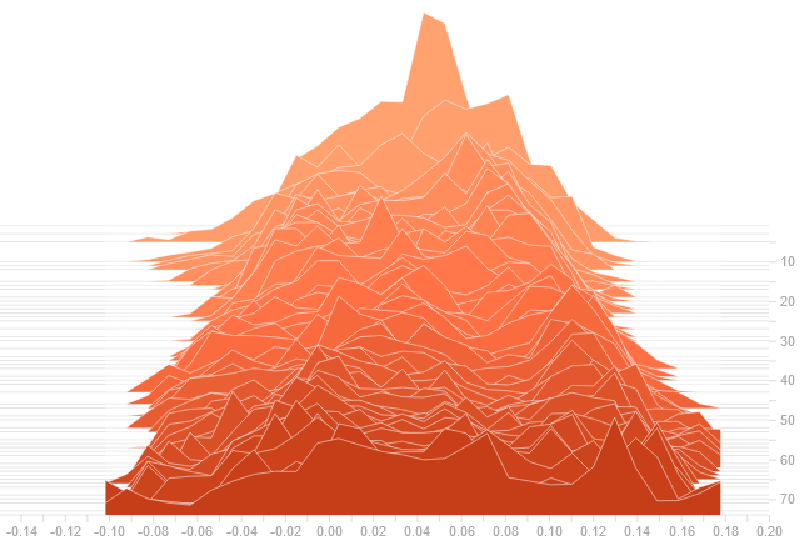
\includegraphics[width=1.0\linewidth]{Figures/LSTM-Bias.pdf}
    \end{subfigure}
    \par\bigskip
    \begin{subfigure}[b]{0.6\linewidth}
        \caption{Training weights per training epoch}
        \label{fig:weight-training}
        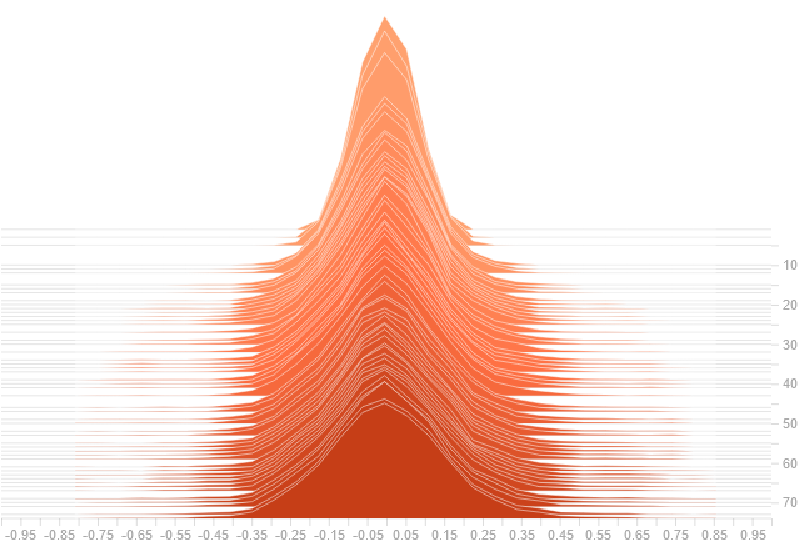
\includegraphics[width=1.0\linewidth]{Figures/LSTM-Weights.pdf}
    \end{subfigure}
\end{figure}

The model training, validation and error comparison with previous model performances took approximately 3 minutes, after which the model predicted the subsequent day's forecast in under 10 seconds. Figure~\ref{fig:lstm-final-data} shows how this looked. The forecaster accurately depicted the initial peaks for the entire day, including the morning, afternoon, and evening. It is clear however, that the rest of the data points may not be as accurate. This is not a significant drawback for the hybrid model, as the reactive algorithm is capable of making minor adjustments to the resources, ensuring that the SLA compliance is maintained.

\begin{comment}
\begin{figure}[htb]
    \centering
    \caption{Example of the forecasted workload}
    \label{fig:lstm-final-data}
    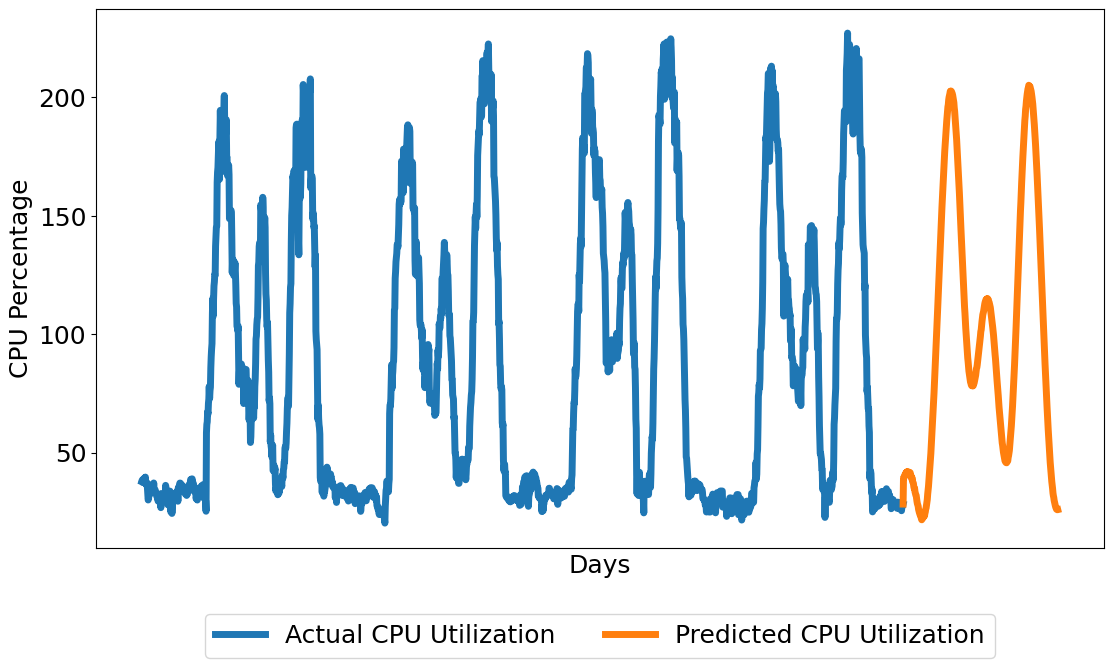
\includegraphics[width=1.0\linewidth]{Figures/LSTM-Final-Data.pdf}
\end{figure}
\end{comment}

\begin{center}
\begin{minipage}{\linewidth}
    \captionof{figure}{Historical workload paired with forecast workload}
    \label{fig:lstm-final-data}
    \begin{tikzpicture}
        \begin{axis}[
            height=0.4\linewidth,
            width=\linewidth,
            xmin=-150,
            xmax=2460,  % Make xmax 150 above the final xtick
            ymin=0,
            ymajorgrids=true,
            yminorgrids=true,
            xmajorgrids=true,
            xminorgrids=true,
            grid style=dashed,
            xlabel={Time (Days)},
            ylabel={CPU Usage (\%)},
            legend style={at={(0.5,-0.3)},anchor=north,legend columns=-1},
            xticklabels={Day 1, Day 2, Day 3, Day 4, Day 5},
            xtick={462, 924, 1386, 1848, 2310}
        ]
            \addplot+[RoyalBlue, mark=none] table [x=xtick, y=value, col sep=comma] {Data/LSTM-Final-Data-Value.csv};
            \addplot+[RedOrange, mark=none] table [x=xtick, y=value, col sep=comma] {Data/LSTM-Final-Data-Forecast.csv};
            %\draw[red, thick, dashed] (axis cs:0, 150) -- (axis cs:2472, 150);
            \legend{Historical workload, Forecast workload}
            %\addlegendimage{line width=0.3mm, dashed, color=red}
            %\addlegendentry{Threshold}
        \end{axis}
    \end{tikzpicture}
\end{minipage}
\end{center}

\subsection{Autoscaler Controller}
\label{subsec:ch5-auto-daemon-subsection}

The autoscaler controller stored a maximum of seven days of data for use by the proactive forecaster. Data that is too old is not particularly useful for a time-series model training on semi-predictable data, and only increases training time without adding much to the accuracy~\cite{greff2016lstm}. This data was refreshed once every day to ensure that the latest data was always available to the hybrid autoscalers before training. Since training only took place once a day, the costly metric scraping operations done by the controller from the cloud layer could be reduced, thereby reducing the overall load on the network.\par

The controller sent a training request to the proactive autoscaler once every night. The time is chosen so that, due to the comparatively low amounts of user requests, the training process would be able to claim as much of the edge resources as possible without affecting the network availability. However, before sending the request, the controller computed whether or not an SLA violation took place in the past 24 hours. If it detected a violation, it assumed that the forecaster had not learnt enough of the time-series features to make an accurate prediction. This could be due to a variety of reasons such as lack of training data or conservative parameter values. To counteract this, the controller performed the following corrections:

\begin{itemize}
    \item $learning\_rate$ was decreased by 0.0005, to a minimum value of 0.002.
    \item $epochs$ was increased by 5, to a maximum of 100.
    \item $batch\_size$ was increased by 10, to a maximum of 200.
    \item $early\_stop$ threshold was increased by 5, to a maximum of 25.
\end{itemize}

The assumption here was that the training accuracy could be jump started by sacrificing short training times for one duration to better learn the time series features and thus reduce SLA violations. As long as SLA violations occur, these modifications keep being performed up until their configured limits. Experimental testing demonstrated that, at the most extreme hyper-parameter configuration, the training time increased to 10 minutes. Once no SLA violations were detected during a 24 hour time window, the hyper-parameters were reverted back to the default values. Doing so did not cause the model to lose any previous optimizations or reduce prediction accuracy, but had the added benefit of reducing training time and resources once again.
\clearpage

\def\chaptertitle{Performance Evaluation}

\lhead{\emph{\chaptertitle}}

\chapter{\chaptertitle}
\label{ch:performance-evaluation}

In this chapter, we begin by discussing the underlying server hardware configuration, and the assumptions made before beginning the auto-scaling experiments in Section~\ref{sec:ch6-hardware-assumptions}. The cluster configuration, which involves the resource divisions between servers, overall cluster architecture, and deployment resources is discussed in Section~\ref{sec:ch6-cluster-config}. The experimental setup which details the SLA categories, its latency values, and an overview of the two experiments to be conducted are discussed in Section~\ref{sec:ch6-exp-setup}. After this, Section~\ref{sec:ch6-baseline-algos} contains an overview of the three baseline algorithms which were used to compare the performance of the proposed hybrid autoscaler. Section~\ref{sec:ch6-exp-workload} follows this with an overview of the workload which was generated to test the two experimental conditions, along with a brief analysis of the latency graph. Finally, the experimental results are shown and discussed in \cref{sec:ch6-request-latency-eval,sec:ch6-cpu-workload-eval,sec:ch6-sla-violation-eval}.

\section{Assumptions and Virtual Machines Setup}
\label{sec:ch6-hardware-assumptions}

For the underlying virtual machine (VM) setup, servers in the Melbourne Research Cloud~\footnote{\url{https://docs.cloud.unimelb.edu.au/}} were leveraged to deploy micro-services on. The setup consisted of 6 VMs, using a total of 24 CPU cores and 80GB of memory. These servers were separated into a cloud and an edge layer. The servers on the cloud layer have a substantially higher amount of CPU cores and memory assigned compared to the servers in the edge layer, to simulate the scarcity of resources in the edge layer. The cloud layer also contained a 200GB persistent storage volume, while the edge layer did not. This allowed the cloud layer to hold all the Prometheus data, while the edge layer had to store the time series in the RAM to depict the scarcity of resources further. Finally, a simulated latency was added between inter-layer server communication to mimic the perceived distance between edge nodes and large data centres.\par

Each server consists of an Ubuntu 22.04~\footnote{\url{https://releases.ubuntu.com/jammy/}} operating system. Kubernetes v1.28.2~\footnote{\url{https://kubernetes.io/releases/}} is used as the container orchestration technology behind the experimental micro service setup. CRI-O was installed on the Kubernetes nodes as the container runtime of choice for running resource nodes. Finally, for inter-pod communication on the cluster to occur, an open-source project known as Flannel~\footnote{\url{https://github.com/flannel-io/flannel}} was deployed.\par

For maximum flexibility in modifying and monitoring the underlying architecture, a bare-metal implementation of Kubernetes was used, instead of ready-made solutions available from Amazon or Google. The control plane was deployed on the cloud layer, while the data plane was on the edge layer. Furthermore, several assumptions were made before proceeding with the experimentation:

\begin{itemize}
    \item The only auto-scaling performed would be horizontal pod auto-scaling. Vertical and cluster auto-scaling were out of the scope of this project.
    \item The pods on which auto-scaling is not applied would have the maximum possible resource allocation, so as to remove the chances of bottleneck.
    \item At no point in the experiment would a node be taken down, or new node be added.
    \item The autoscaler assumes that every node in the edge layer is an equally likely candidate for scheduling pods on.
\end{itemize}

\section{Cluster Configurations}
\label{sec:ch6-cluster-config}

The VMs were divided into the cloud and edge layer as depicted in Table~\ref{tab:cluster-hw-overview}. The control plane was further divided into two servers, one for handling the Kubernetes control plane scheduling, API service, and etcd deployments, and the other for storing the Prometheus database, along with the micro-service Jaeger metrics collection. The edge layer consisted of four servers with far substantially fewer resources, to depict the difference in computing power. The network layer between the edge and cloud deployments also contained a simulated latency to denote the perceived geographical distance between them.\par

%TC:ignore
\begin{table}
    \caption{Cluster architectural layout}\label{tab:cluster-hw-overview}
    \centering
    \begin{tabular}{cccc}
        \toprule
        \textbf{Node} & \textbf{Layer} & \textbf{CPU (cores)} & \textbf{Memory (GB)}\\
        \midrule
        Control-Plane-K8s & Cloud & 8 & 32\\
        Control-Plane-DB  & Cloud & 8 & 32\\
        Data-Plane-1      & Edge  & 2 & 4\\
        Data-Plane-2      & Edge  & 2 & 4\\
        Data-Plane-3      & Edge  & 2 & 4\\
        Data-Plane-4      & Edge  & 2 & 4\\
        \toprule
    \end{tabular}
\end{table}
%TC:endignore

The cloud and edge nodes were differentiated through Kubernetes through the internal labeling system. A key \textit{type} with the value either \textit{cloud} or \textit{edge} was added to each node. This would enable the scheduler to consider restricting the deployment of pods to particular nodes automatically. For example, the Prometheus deployment would only be deployed on the node of the type cloud. This process is known as \textit{node affinity}~\cite{santos2019towards}.\par

There were several options to deploy the social media application to Kubernetes. Manually cloning them from the repository, creating the custom resource definitions (CRDs), and deploying the YAML files was an option that gave maximum flexibility, but was difficult to debug if things went wrong. Due to this, the Kubernetes package manager Helm was used. Helm~\footnote{\url{https://helm.sh/}} is another open-source project whose primary goal involves streamlining the installation, maintenance, and removal of Kubernetes deployments. This is achieved through the use of a Helm chart, which details the configuration of the project, and how to update and access it.\par

Therefore, the social media application was the first to be deployed on Kubernetes. However, before deploying the application, the primary deployments to be tested need to be configured. Based on the \textit{wrk2} benchmark that was discussed above, two APIs were identified. One was a GET call to the user's home timeline, and the other was a POST request made by the user to create a post.\par

First, the social network with default configuration values was installed using the helm command below:

\begin{lstlisting}[
  caption={Social network installation using Helm},
  captionpos=t,
  label={lst:social-network-helm-install},
  language=bash
]
$ helm install social-media \
/DeathStarBench/socialNetwork/helm-chart/Chart.yaml -n default
\end{lstlisting}

With the social media network now deployed, a workload for both GET and POST requests was invoked to generate the latency trace on Jaeger, as depicted in Listing~\ref{lst:wrk2-api-calls}.

\begin{lstlisting}[
  caption={Generate Jaeger trace},
  captionpos=t,
  label={lst:wrk2-api-calls},
  float=ht,
  language=bash
]
$ WRK2="/DeathStarBench/wrk2/wrk -D exp -t 1 -c 1 -d 1 -L -s -R 1"
$ HT=./wrk2/scripts/social-network/read-home-timeline.lua
$ CS=./wrk2/scripts/social-network/compose-post.lua
$ IP=$(kubectl get svc nginx-thrift --template '{{.spec.clusterIP}}')
$ PORT=8080
$ $WRK2 $HT http://$IP:$PORT/wrk2-api/home-timeline/read
$ $WRK2 $HT http://$IP:$PORT/wrk2-api/post/compose
\end{lstlisting}

With the traces generated, the deployments that require auto-scaling could be identified for each. From the Jaeger traces generated in Figure~\ref{fig:ht-cp-trace}, it was clear that the two deployments highlighted in pink, namely \textit{home-timeline-service}, and \textit{compose-post-service}, were the major bottlenecks in GET and POST request processing respectively, having to serve multiple child deployments simultaneously. This made them the most important deployments for auto-scaling. Therefore, the helm deployment was updated to assign auto-scaling resource limits to them. The resources were assigned in a realistic manner consistent with edge deployments and based on the number of components each deployment answered to. Listing~\ref{lst:deploy-resource-update} shows the CPU resources assigned to both deployments.\par

\begin{minipage}{\linewidth}
    \begin{lstlisting}[
      caption={Update resources for bottlenecked deployments},
      captionpos=t,
      label={lst:deploy-resource-update},
      language=bash
    ]
    $ helm upgrade social-media \
    /DeathStarBench/socialNetwork/helm-chart/Chart.yaml -n default \
    --set-string home-timeline-service.container.resources="requests: 
          cpu: "15m"
        limits:
          cpu: "15m"" \
    --set-string compose-post-service.container.resources="requests: 
          cpu: "30m"
        limits:
          cpu: "30m""
    \end{lstlisting}
\end{minipage}

\begin{figure}[htb]
    \centering
    \caption{API trace for \textit{home-timeline-service} and \textit{compose-post-service}}
    \label{fig:ht-cp-trace}
    \begin{minipage}{0.25\linewidth}
        %\caption{Home Timeline API trace}
        %\label{fig:home-timeline-trace}
        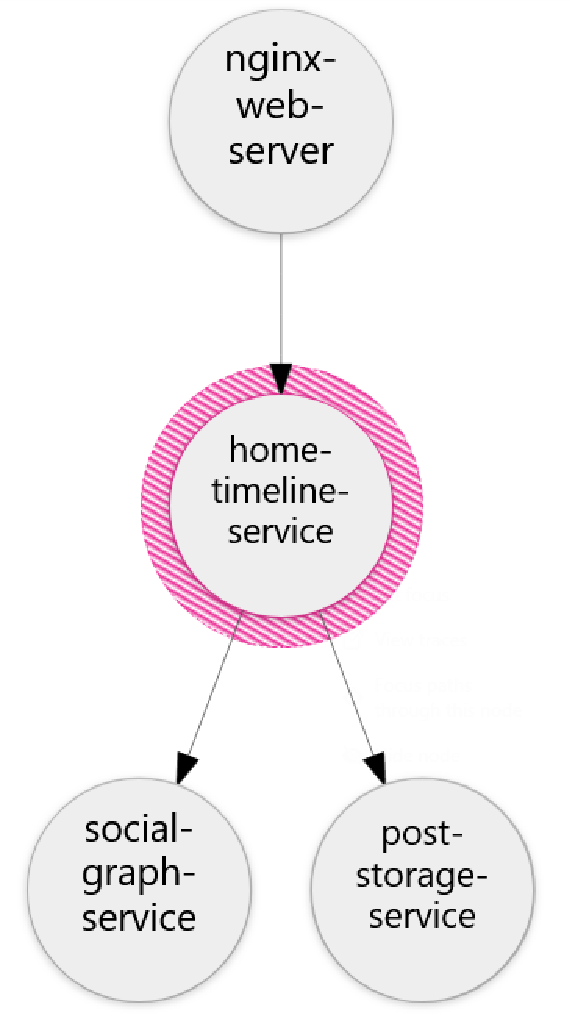
\includegraphics[width=1.0\linewidth]{Figures/Home-Timeline-GET-Trace.pdf}
    \end{minipage}\hfill
    \begin{minipage}{0.75\linewidth}
        %\caption{Compose Post API trace}
        %\label{fig:compose-post-trace}
        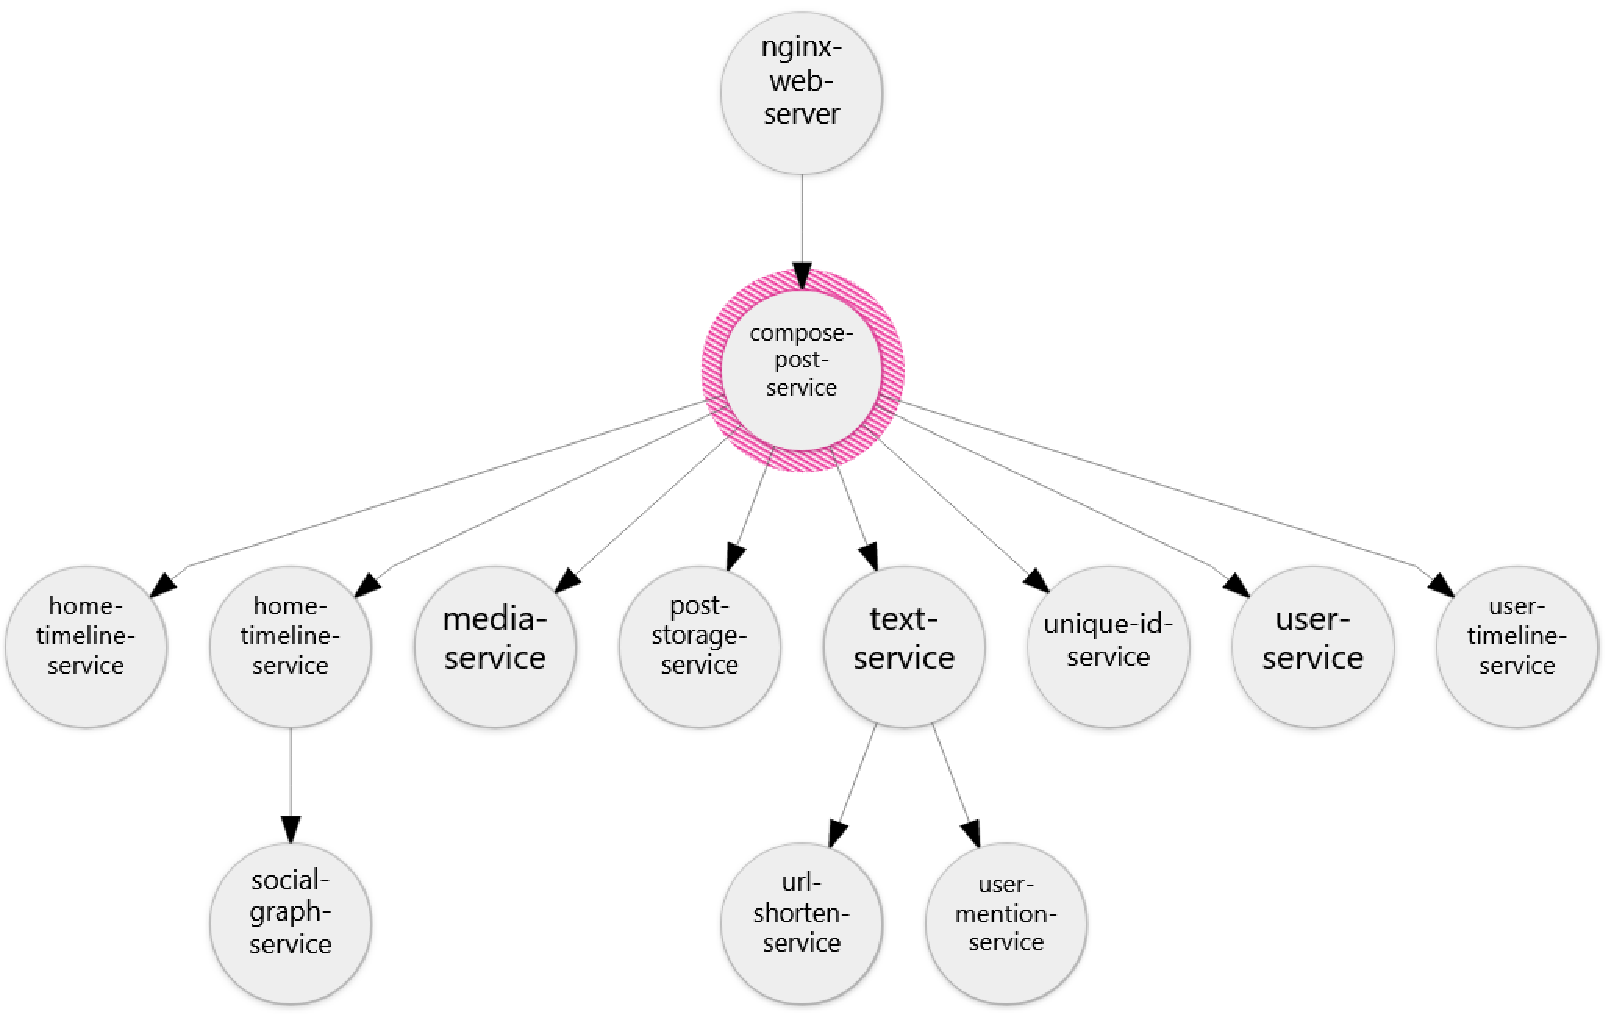
\includegraphics[width=1.0\linewidth]{Figures/Compose-Post-POST-Trace.pdf}
    \end{minipage}
\end{figure}

\section{Experiment Setup}
\label{sec:ch6-exp-setup}

Two independent experiments were conducted to validate the performance of the hybrid autoscaler. The social media application was first tested using the GET request to the API to autoscale the \textit{home-timeline-service} deployment. Then, a more demanding as well as challenging workload was applied to the POST request for auto-scaling the \textit{compose-post-service} deployment. For both these experiments, the workload generation algorithm was used to create realistic daily workloads and tested over a period of five days.

According to Nilsson and Yngwe~\cite{nilsson2022api}, their research concluded that user experience was negatively affected by higher API latency. This leads to a cascading issue of lower revenue growth and profit. Their research found three latency brackets where the user experience changes.

\begin{itemize}
    \item A response time of at least \textit{100 milliseconds} was considered by the user to be instantaneous. This is the best case scenario.
    \item A response time of up to \textit{1 second} was noticed by the user as a slight delay, however their user experience was not significantly interrupted.
    \item A response time exceeding \textit{10 seconds} was deemed to cause the user to lose focus, and thus disrupted their user experience.
\end{itemize}

Based on this research, it was determined that for both the experiments, the flexible, moderate, and strict SLA constraints explained in Section~\ref{subsec:ch4-problem-formulation} would be bound within the values $SLA(c) \in [100ms, 1000ms]$.\par

The flexible SLA constraint was the primary focus of the experiment. This threshold was chosen as it is the most common threshold used for IoT applications, and thus provide a good benchmark for application performance. However, a moderate and strict SLA constraint would also be chosen and tested to compute the SLA violation rates for the algorithm. The SLA values are shown in Table~\ref{tab:experiment-sla-values}.\par

%TC:ignore
\begin{table}
    \caption{Experimental SLA constraints}\label{tab:experiment-sla-values}
    \centering
    \begin{tabular}{ccc}
        \toprule
        \textbf{SLA Type} & \textbf{GET latency(ms)} & \textbf{POST latency(ms)}\\
        \midrule
        Flexible    & 150   & 1000\\
        Moderate    & 125   & 900\\
        Strict      & 100   & 800\\
        \toprule
    \end{tabular}
\end{table}
%TC:endignore

For the proposed hybrid algorithm to achieve these auto-scaling goals within the SLA constraints, the auto-scaling subsystems were configured as follows. The reactive autoscaler would check if the CPU utilization of the deployment was exceeding the auto-scaling threshold. This threshold would vary for each of the experiments as required. If this threshold was breached, it would scale up based on the cooldowns and tolerations set. The proactive autoscaler on the other hand would check if the forecasted CPU utilization in the next 20 minutes was going to breach the auto-scaling threshold, and if so, would autoscale with the same configured parameters as the reactive one. The controller would store the total CPU utilization of the deployment as a time-series for a maximum of seven days, and constantly check for SLA violations to tweak the hyper-parameters of the forecaster as discussed above in Section~\ref{subsec:ch5-auto-daemon-subsection}.\par

\section{Baseline Algorithms}
\label{sec:ch6-baseline-algos}

To measure the effectiveness of the hybrid autoscaler, three baseline algorithms were chosen for comparison. All three would autoscale at the same CPU auto-scaling threshold to maintain consistency. Furthermore, these algorithms would be implementations based on the ones discussed in \cref{sec:ch3-reactive-solutions,sec:ch3-proactive-solutions}.\par

\begin{enumerate}
    \item \textbf{Default Kubernetes Horizontal Pod Autoscaler}: No modifications to the configuration are made, thus the scale-up cooldown is 0 seconds, while the scale-down is 300 seconds. Additionally, the autoscaler has no knowledge of the workload distribution or SLA violations on the edge nodes.
    \item \textbf{Traffic Aware Horizontal Pod Autoscaler}: This is an implementation of the reactive THPA algorithm created by Phan \textit{et al}.~\cite{phan2022traffic}. This autoscaler scheduler will compute the ratio of workloads being exerted on the different edge nodes with the deployment pods. Once it does so, it will scale these resources in a commensurate proportion.
    \item \textbf{Proactive Pod Autoscaler}: This is an implementation of the PPA algorithm devised by Ju \textit{et al}.~\cite{ju2021proactive}. This algorithm was an open-ended implementation that enabled the user to plugin a deep learning model of their choice. The PPA architecture consists of three sub-sections, the formulator, evaluator, and updater. An LSTM model is injected into the autoscaler as the model file. This LSTM implementation is similar to the one used in the hybrid autoscaler, however, it differs in two key elements. First, the LSTM does not expect pre-processed data without noise and thus deals with more complex time-series data. Secondly, due to this additional computation, the LSTM contains a deeper architecture layer with more neural network units. This is required as the algorithm has to correctly predict the complete future workload since there is no reactive autoscaler to fall back on. Over a fixed interval, the algorithm continuously loops through the time-series data and saves the forecast result to a metrics file. The evaluator takes these outputs from the metrics file, along with the LSTM from the model file to predict the number of pods to assign in advance, and requests the Kubernetes scheduler for scaling through the API Service. A second loop, known as the update loop, then updates the LSTM model using the latest forecast, and clears the metrics file. The hyper-parameters are carefully tuned to ensure that the model does not underperform. Finally, the PPA architecture does not take into account SLA compliance, and thus SLA metrics are not provided as feedback for hyper-parameter tuning.
\end{enumerate}

\section{Experimental Workload}
\label{sec:ch6-exp-workload}

In the first experiment, the IoT workload generation algorithm was configured to create a workload aimed at mimicking GET requests. By doing so, the \textit{home-timeline-service} deployment became the bottleneck receiving all of the requests and thus could be tested using the proposed hybrid autoscaler, as well as the three baseline algorithms. As explained above, the auto-scaling threshold for all four algorithms was set to 50\% total CPU utilization on the deployment, and the SLA latency threshold was set to the flexible threshold of 150 milliseconds.\par

\begin{comment}
\begin{figure}[htb]
    \centering
    \caption{Total CPU utilization for home-timeline-service}
    \label{fig:exp1-workload}
    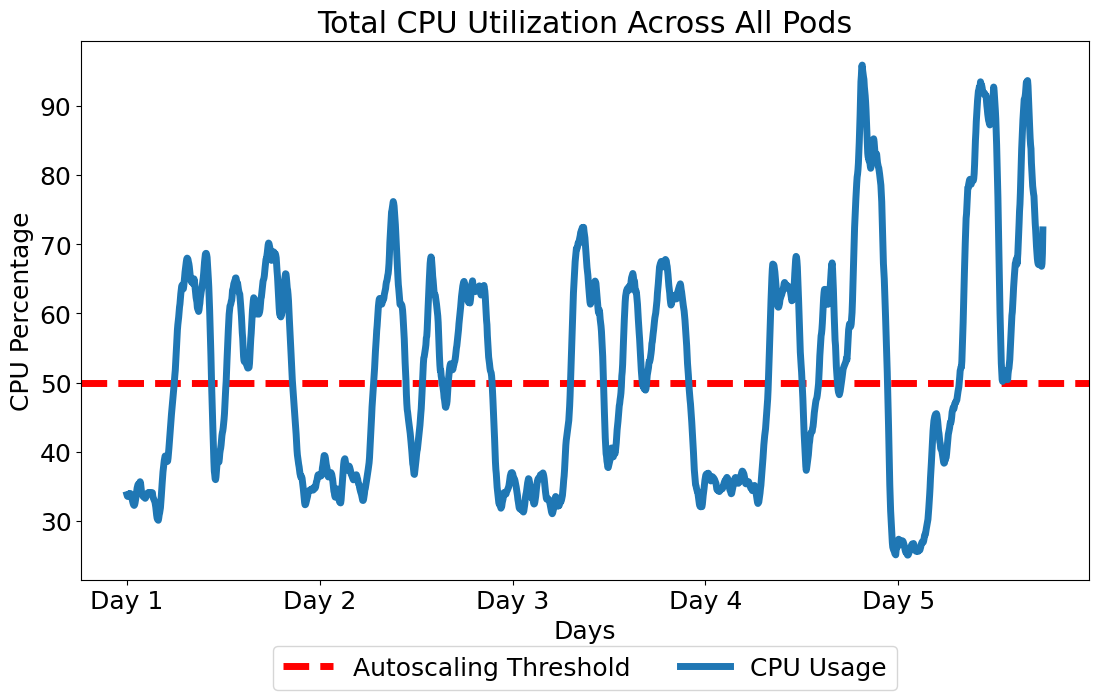
\includegraphics[width=0.6\linewidth]{Figures/GET-Total-CPU.pdf}
\end{figure}
\end{comment}

\begin{center}
\begin{minipage}{\linewidth}
    \captionof{figure}{Total CPU utilization for \textit{home-timeline-service}}
    \label{fig:exp1-workload}
    \begin{tikzpicture}
        \begin{axis}[
            height=0.4\linewidth,
            width=\linewidth,
            xmin=0,
            xmax=2460,  % Make xmax 150 above the final xtick
            ymin=0,
            ymajorgrids=true,
            yminorgrids=true,
            xmajorgrids=true,
            xminorgrids=true,
            grid style=dashed,
            xlabel={Time (Days)},
            ylabel={CPU Usage (\%)},
            legend style={at={(0.5,-0.3)},anchor=north,legend columns=-1},
            xticklabels={Day 1, Day 2, Day 3, Day 4, Day 5},
            xtick={570, 1030, 1510, 1950, 2370}
        ]
            \addplot+[RoyalBlue, mark=none] table [x=xtick, y=value, col sep=comma] {Data/GET-Total-CPU.csv};
            \draw[red, thick, dashed] (axis cs:0, 50) -- (axis cs:2460, 50);
            \legend{CPU Usage}
            \addlegendimage{line width=0.3mm, dashed, color=red}
            \addlegendentry{Autoscaling Threshold}
        \end{axis}
    \end{tikzpicture}
\end{minipage}
\end{center}

Figure~\ref{fig:exp1-workload} shows the total CPU workload that was generated by Algorithm~\ref{alg:work-gen} on the \textit{home-timeline-service} deployment. The data was generated for a total of five days. Throughout the five days, approximately \num[group-separator={,}]{2550000} requests in total were sent to the edge deployment. The daily peak remained at approximately the same percentage but then increased significantly in the last two days. This could be interpreted as a depiction of how social network requests may look on the weekends. The total CPU utilization never exceeded 95\% of the total allocated resources shown in Listing~\ref{lst:deploy-resource-update}. This is expected of a GET request, as while the deployment has to open a connection to the sub-deployments to receive the response, a GET request is typically a database SELECT statement, which takes a comparatively less amount of time as opposed to other operations. This means that the deployment can quickly receive the response from its child components, send the response up to the requester, and then close the connection. Once the connection is closed, all the resources associated with it are freed. Because this operation is so quick, multiple concurrent connections are typically not open, and thus the CPU utilization is not significant.\par

For the second experiment, the focus was on a more difficult auto-scaling task. The IoT workload generation Algorithm~\ref{alg:work-gen} was reconfigured to simulate a realistic workload for social network users writing user timeline posts, which at a low level, involved sending POST requests to the edge deployment. Doing so meant that the \textit{compose-post-service} would be sending all these POST requests to its sub-components for writing media or text. The workflow for a POST request to the API goes as follows. The user sends a POST request with the body containing the data to be written. This is sent to the \textit{compose-post-service} deployment which opens an ephemeral connection with the user. Simultaneously while doing so, the deployment sends the contents of the POST body to one of its sub-components. These components house the database for user posts, and the operation is performed using an INSERT or UPDATE statement. The sub-component then sends its response back to the \textit{compose-post-service} informing it whether or not this operation succeeded or failed. The deployment sends this information back up to the user and closes the connection.\par

\begin{comment}
\begin{figure}[htb]
    \centering
    \caption{Total CPU utilization For \textit{compose-post-service}}
    \label{fig:exp2-workload}
    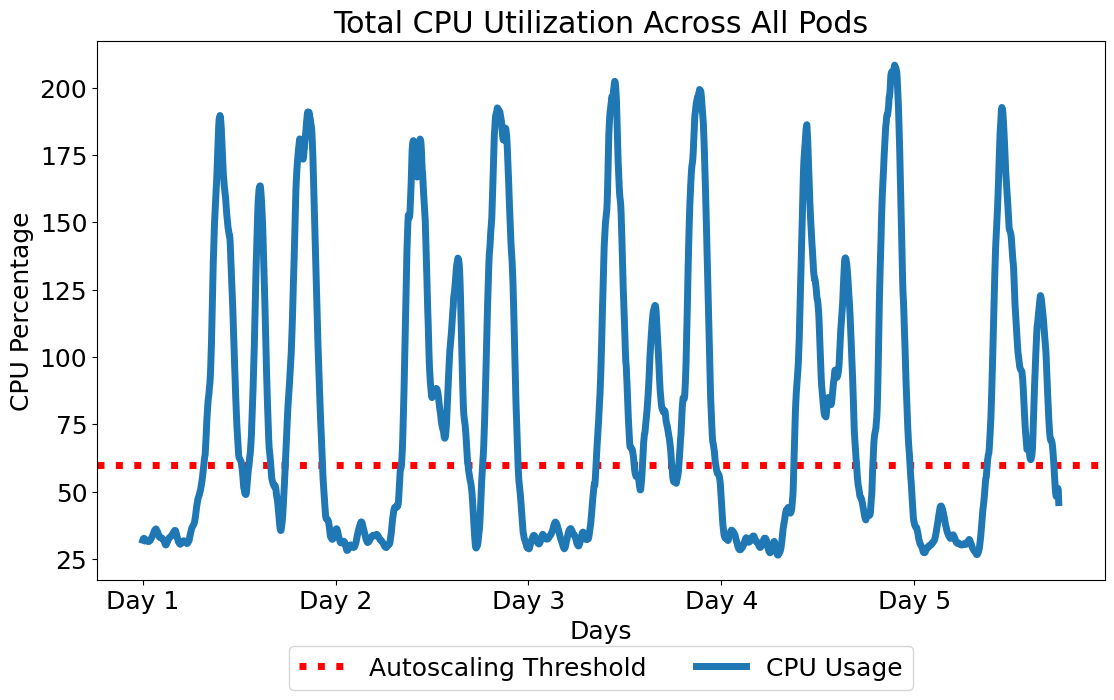
\includegraphics[width=0.6\linewidth]{Figures/POST-Total-CPU.pdf}
\end{figure}
\end{comment}

\begin{center}
\begin{minipage}{\linewidth}
    \captionof{figure}{Total CPU utilization for \textit{compose-post-service}}
    \label{fig:exp2-workload}
    \begin{tikzpicture}
        \begin{axis}[
            height=0.4\linewidth,
            width=\linewidth,
            xmin=0,
            xmax=2460,  % Make xmax 150 above the final xtick
            ymin=0,
            ymajorgrids=true,
            yminorgrids=true,
            xmajorgrids=true,
            xminorgrids=true,
            grid style=dashed,
            xlabel={Time (Days)},
            ylabel={CPU Usage (\%)},
            legend style={at={(0.5,-0.3)},anchor=north,legend columns=-1},
            xticklabels={Day 1, Day 2, Day 3, Day 4, Day 5},
            xtick={580, 1050, 1510, 1970, 2370},
            ytick={0, 60, 120, 180, 240}
        ]
            \addplot+[RoyalBlue, mark=none] table [x=xtick, y=value, col sep=comma] {Data/POST-Total-CPU.csv};
            \draw[red, thick, dashed] (axis cs:0, 60) -- (axis cs:2460, 60);
            \legend{CPU Usage}
            \addlegendimage{line width=0.3mm, dashed, color=red}
            \addlegendentry{Autoscaling Threshold}
        \end{axis}
    \end{tikzpicture}
\end{minipage}
\end{center}

While the SELECT statement used underneath the GET request was a fairly quick operation, the INSERT and UPDATE statements may take significantly longer, due to the idempotent nature of the database~\cite{lutteroth2009database}. The social network will ensure that user posts are in the correct order, and perform other background checks before committing the data. Due to this, the connections on the \textit{compose-post-service} can remain open for a significantly longer amount of time, resulting in far more resources being used. Figure~\ref{fig:exp2-workload} shows this in action. The algorithm was generated for a total of 5 days, similar to the first experiment. Even though the workload generation algorithm was sending the same amount of POST requests as it did GET requests, approximately \num[group-separator={,}]{2550000} requests in total, the total CPU workload in the second experiment peaked at approximately 175\%, and at some points even reached 200\% of the total CPU resources assigned to a unitary deployment pod. This varied per day in a realistic manner similar to what could commonly be seen in social networks.\par

To resolve this CPU bottleneck, the auto-scaling threshold was set to 60\% of the CPU workload. In addition, the SLA latency threshold was set to the flexible threshold of 1000 milliseconds. Using these configurations, the three baseline algorithms along with the proposed hybrid autoscaler was tested.\par

\section{Evaluation of Request Latency}
\label{sec:ch6-request-latency-eval}

\subsection {Default Kubernetes Autoscaler Baseline}
\label{subsec:ch6-default-algo}

\begin{comment}
\begin{figure}[htb]
    \centering
    \caption{Kubernetes Default Autoscaler Latency For \textit{home-timeline-service}}
    \label{fig:exp1-default-k8s}
    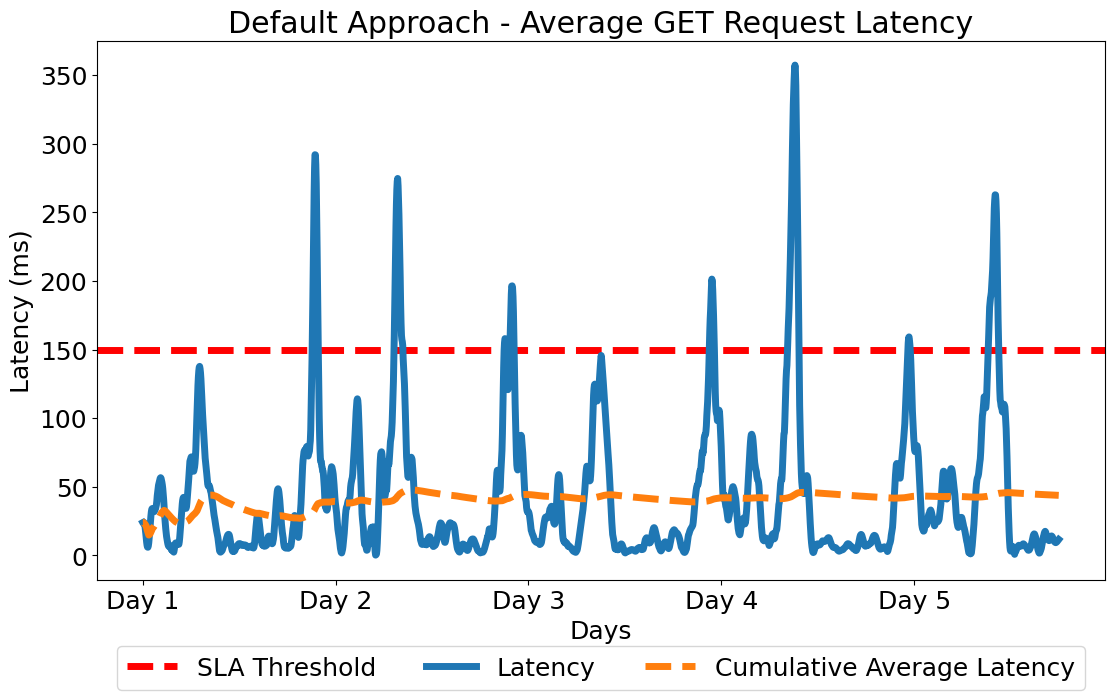
\includegraphics[width=0.6\linewidth]{Figures/Home-Timeline-Default-Latency.pdf}
\end{figure}
\end{comment}

\begin{center}
\begin{minipage}{\linewidth}
    \captionof{figure}{Kubernetes default sutoscaler latency for \textit{home-timeline-service}}
    \label{fig:exp1-default-k8s}
    \begin{tikzpicture}
        \begin{axis}[
            height=0.4\linewidth,
            width=\linewidth,
            xmin=0,
            xmax=2460,  % Make xmax 150 above the final xtick
            ymin=0,
            ymajorgrids=true,
            yminorgrids=true,
            xmajorgrids=true,
            xminorgrids=true,
            grid style=dashed,
            xlabel={Time (Days)},
            ylabel={Latency (ms)},
            legend style={at={(0.5,-0.3)},anchor=north,legend columns=-1},
            xticklabels={Day 1, Day 2, Day 3, Day 4, Day 5},
            xtick={570, 1030, 1510, 1950, 2370},
            ytick={0, 75, 150, 225, 300, 375}
        ]
            \addplot+[RoyalBlue, mark=none] table [x=xtick, y=value, col sep=comma] {Data/Home-Timeline-Default-Latency-CPU.csv};
            \addplot+[OliveGreen, mark=none] table [x=xtick, y=value, col sep=comma] {Data/Home-Timeline-Default-Latency-AVG.csv};
            \draw[red, thick, dashed] (axis cs:0, 150) -- (axis cs:2460, 150);
            \legend{Latency, Cumulative Average Latency}
            \addlegendimage{line width=0.3mm, dashed, color=red}
            \addlegendentry{SLA Threshold}
        \end{axis}
    \end{tikzpicture}
\end{minipage}
\end{center}

For both the workloads discussed above, a near 100\% CPU utilization on a solitary deployment pod would lead to significant delays. This can be seen when using the default Kubernetes Horizontal Pod Autoscaler in the first experiment, as depicted in Figure~\ref{fig:exp1-default-k8s}. The autoscaler was merely a primitive reactive implementation with no knowledge of which edge nodes were experiencing heavy traffic, and which ones were not. Thus, it blindly assigned pods to the nodes in a round-robin manner. Additionally, the autoscaler required a significant amount of time to register the new pods to the Kubernetes control plane, thus falling victim to the cold start problem. This results in significant latency spikes before the resources are adjusted. In the figure, it can be seen that the latency exceeds 300 milliseconds at some points, which would be significantly large enough to degrade the user experience. Additionally, by the end of the fifth day of testing, the cumulative average latency of the social-network was nearly 50 milliseconds.\par

\begin{comment}
\begin{figure}[htb]
    \centering
    \caption{Kubernetes Default Autoscaler Latency For \textit{compose-post-service}}
    \label{fig:exp2-default-k8s}
    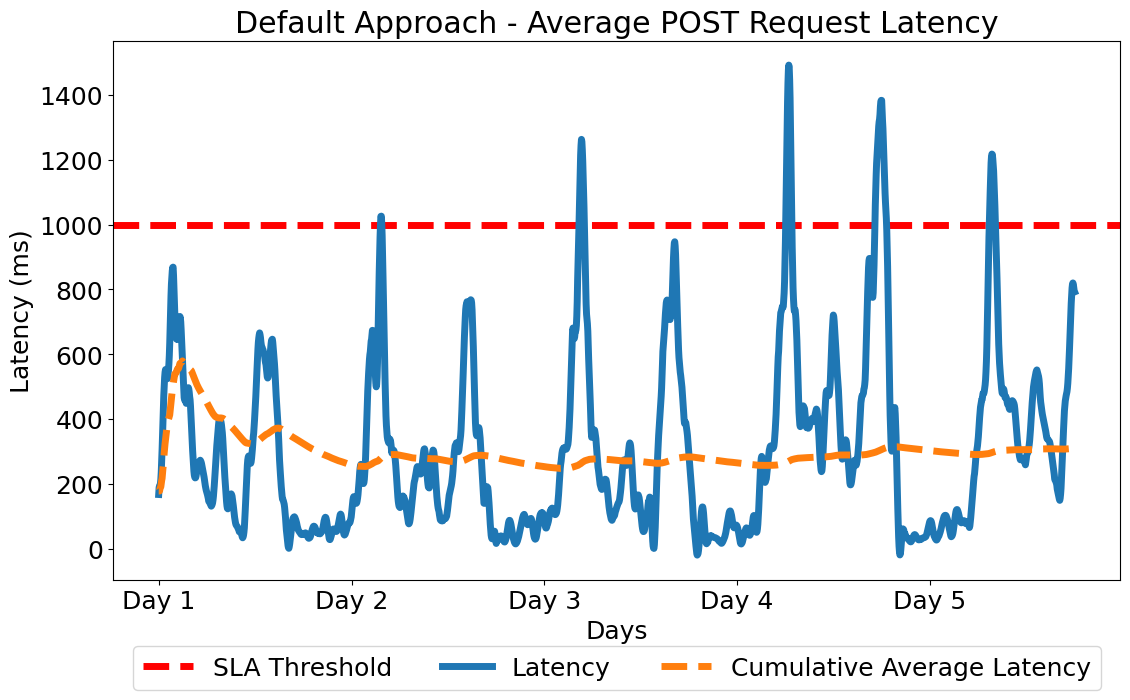
\includegraphics[width=0.6\linewidth]{Figures/Compose-Post-Default-Latency.pdf}
\end{figure}
\end{comment}

\begin{center}
\begin{minipage}{\linewidth}
    \captionof{figure}{Kubernetes default autoscaler latency for \textit{compose-post-service}}
    \label{fig:exp2-default-k8s}
    \begin{tikzpicture}
        \begin{axis}[
            height=0.4\linewidth,
            width=\linewidth,
            xmin=0,
            xmax=2460,  % Make xmax 150 above the final xtick
            ymin=0,
            ymajorgrids=true,
            yminorgrids=true,
            xmajorgrids=true,
            xminorgrids=true,
            grid style=dashed,
            xlabel={Time (Days)},
            ylabel={Latency (ms)},
            legend style={at={(0.5,-0.3)},anchor=north,legend columns=-1},
            xticklabels={Day 1, Day 2, Day 3, Day 4, Day 5},
            xtick={580, 1050, 1510, 1970, 2370}
        ]
            \addplot+[RoyalBlue, mark=none] table [x=xtick, y=value, col sep=comma] {Data/Compose-Post-Default-Latency-CPU.csv};
            \addplot+[OliveGreen, mark=none] table [x=xtick, y=value, col sep=comma] {Data/Compose-Post-Default-Latency-AVG.csv};
            \draw[red, thick, dashed] (axis cs:0, 1000) -- (axis cs:2460, 1000);
            \legend{Latency, Cumulative Average Latency}
            \addlegendimage{line width=0.3mm, dashed, color=red}
            \addlegendentry{SLA Threshold}
        \end{axis}
    \end{tikzpicture}
\end{minipage}
\end{center}

Similar to the results in the first experiment, the shortcomings of this auto-scaling approach were exposed even more so by the increased demands of the POST request workload in the second experiment. Figure~\ref{fig:exp2-default-k8s} shows the latency metrics of the autoscaler. During the daily workload spikes, the autoscaler would regularly breach the 1000 millisecond threshold, with values peaking at almost 1450 milliseconds. This is more than 45\% above the allowed threshold, which would cause general system instability. Furthermore, the average latency of the autoscaler hovered at around the 400-millisecond mark throughout the experiment, which was quite a high value when taking into account the large periods of non-peak workload in the test.\par

Upon further investigation, it was discovered that the high latency was caused due to three issues. One was the cold start problem, which added a constant latency to the non-proactive algorithms which could not be solved by any reactive solutions. The second one was the avalanche effect which was caused by resources not being available in a timely manner, and was related to the cold start. Before the Kubernetes control plane could register all resources, the \textit{compose-post-service} deployment may have had a CPU utilization at or near 100\%. When this happened, the deployment already had all available resources being utilized to open connections, this caused additional connection requests to be dropped. The user does not see this happen and instead waits the default 60 seconds before displaying a ``time-out'' message. This 60 seconds was taken into account when measuring the latency and was what drove up the latency to such an extent. Finally, the Kubernetes default autoscaler had no information on which edge nodes were receiving the most number of requests. It only saw CPU utilization metrics as a totality. As a result of this, it scheduled new resources in a round-robin manner, meaning that some deployment pods received a lot of requests, while others may have received none. This uneven distribution of requests to the resources also drove up latency.\par

Based on these experimental results which showed that connections were being dropped, it meant that the social network was becoming unavailable at certain points in time during the day. This happening during peak hours was especially critical and violated SLA constraints. Due to this, the default Kubernetes autoscaler could not be considered viable for auto-scaling an edge deployment.

\subsection {Reactive THPA Autoscaler Baseline}
\label{subsec:ch6-reactive-algo}

\begin{comment}
\begin{figure}[htb]
    \centering
    \caption{THPA Reactive Autoscaler Latency For \textit{home-timeline-service}}
    \label{fig:exp1-reactive-k8s}
    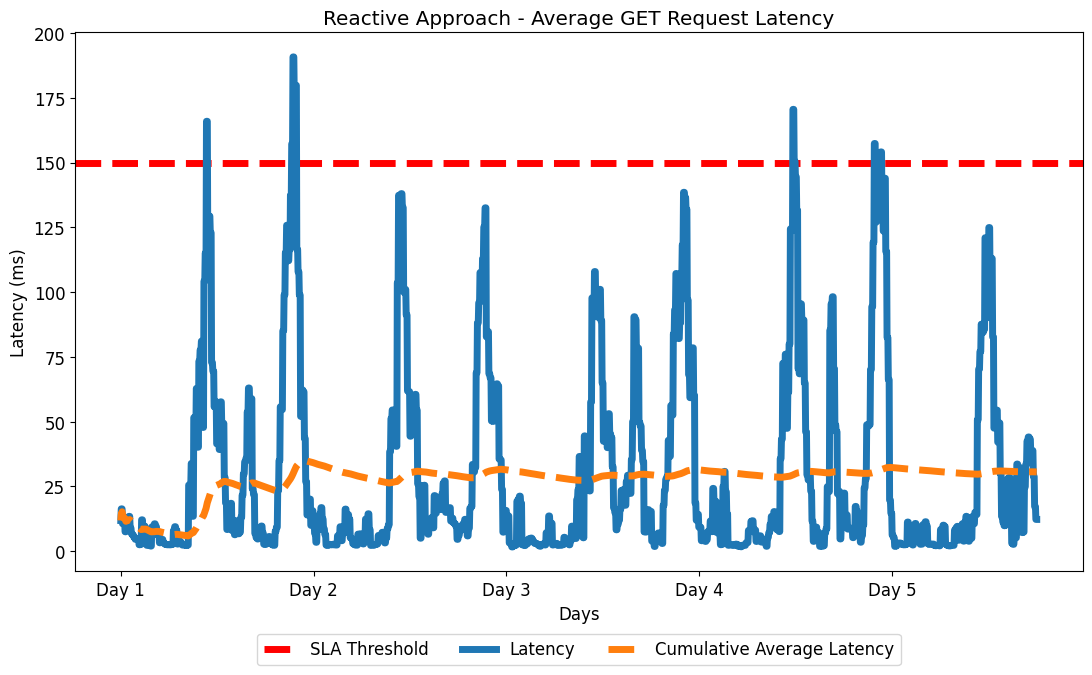
\includegraphics[width=0.6\linewidth]{Figures/Home-Timeline-Reactive-Latency.pdf}
\end{figure}
\end{comment}

\begin{center}
\begin{minipage}{\linewidth}
    \captionof{figure}{THPA reactive autoscaler latency for \textit{home-timeline-service}}
    \label{fig:exp1-reactive-k8s}
    \begin{tikzpicture}
        \begin{axis}[
            height=0.4\linewidth,
            width=\linewidth,
            xmin=0,
            xmax=2460,  % Make xmax 150 above the final xtick
            ymin=0,
            ymajorgrids=true,
            yminorgrids=true,
            xmajorgrids=true,
            xminorgrids=true,
            grid style=dashed,
            xlabel={Time (Days)},
            ylabel={Latency (ms)},
            legend style={at={(0.5,-0.3)},anchor=north,legend columns=-1},
            xticklabels={Day 1, Day 2, Day 3, Day 4, Day 5},
            xtick={570, 1030, 1510, 1950, 2370}
        ]
            \addplot+[RoyalBlue, mark=none] table [x=xtick, y=value, col sep=comma] {Data/Home-Timeline-Reactive-Latency-CPU.csv};
            \addplot+[OliveGreen, mark=none] table [x=xtick, y=value, col sep=comma] {Data/Home-Timeline-Reactive-Latency-AVG.csv};
            \draw[red, thick, dashed] (axis cs:0, 150) -- (axis cs:2460, 150);
            \legend{Latency, Cumulative Average Latency}
            \addlegendimage{line width=0.3mm, dashed, color=red}
            \addlegendentry{SLA Threshold}
        \end{axis}
    \end{tikzpicture}
\end{minipage}
\end{center}

Unlike the default Kubernetes autoscaler, THPA kept track of which edge node was receiving a significant number of requests and assigned pods to the nodes accordingly. This strategy resulted in a significantly improved latency graph for the first experiment, as can be seen in Figure~\ref{fig:exp1-reactive-k8s}.\par

While the algorithm still suffered from the cold start problem, the more intelligent assignment of resources resulted in fewer availability issues, ensuring that the latency spikes that were seen were not as drastic as the ones in the default implementation. However, due to the cold start problem, the SLA threshold of 150 millisecond was still regularly breached, resulting in several violations and degraded the user experience. However these breaches never exceeded the 200 millisecond mark, and thus the drop in user experience quality was not as noticeable as the approach using the default Kubernetes baseline. Furthermore, the average latency over the experimental time frame was lower than what was seen in the default implementation, hovering at around 25-30 milliseconds.\par

\begin{comment}
\begin{figure}[htb]
    \centering
    \caption{THPA Reactive Autoscaler Latency For \textit{compose-post-service}}
    \label{fig:exp2-reactive-k8s}
    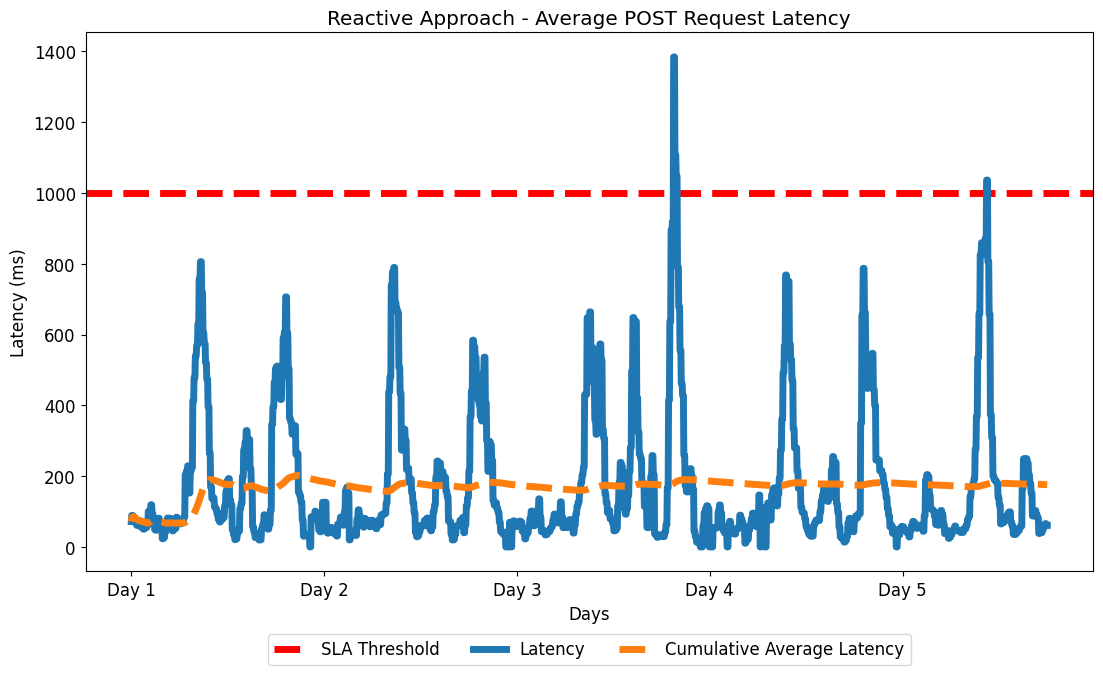
\includegraphics[width=0.6\linewidth]{Figures/Compose-Post-Reactive-Latency.pdf}
\end{figure}
\end{comment}

\begin{center}
\begin{minipage}{\linewidth}
    \captionof{figure}{THPA reactive autoscaler latency for \textit{compose-post-service}}
    \label{fig:exp2-reactive-k8s}
    \begin{tikzpicture}
        \begin{axis}[
            height=0.4\linewidth,
            width=\linewidth,
            xmin=0,
            xmax=2460,  % Make xmax 150 above the final xtick
            ymin=0,
            ymajorgrids=true,
            yminorgrids=true,
            xmajorgrids=true,
            xminorgrids=true,
            grid style=dashed,
            xlabel={Time (Days)},
            ylabel={Latency (ms)},
            legend style={at={(0.5,-0.3)},anchor=north,legend columns=-1},
            xticklabels={Day 1, Day 2, Day 3, Day 4, Day 5},
            xtick={580, 1050, 1510, 1970, 2370}
        ]
            \addplot+[RoyalBlue, mark=none] table [x=xtick, y=value, col sep=comma] {Data/Compose-Post-Reactive-Latency-CPU.csv};
            \addplot+[OliveGreen, mark=none] table [x=xtick, y=value, col sep=comma] {Data/Compose-Post-Reactive-Latency-AVG.csv};
            \draw[red, thick, dashed] (axis cs:0, 1000) -- (axis cs:2460, 1000);
            \legend{Latency, Cumulative Average Latency}
            \addlegendimage{line width=0.3mm, dashed, color=red}
            \addlegendentry{SLA Threshold}
        \end{axis}
    \end{tikzpicture}
\end{minipage}
\end{center}

Figure~\ref{fig:exp2-reactive-k8s} shows how the THPA algorithm performed on the POST request workload for the second experiment. As expected, the request-aware architecture of this autoscaler allowed it to eliminate the issues with dropped requests seen in the Kubernetes autoscaler implementation. This was due to the autoscaler assigning resource pods to the edge nodes which were experiencing a high number of POST requests. This ensured that on average, the latency values were kept lower. Furthermore, the avalanche effect seen above was somewhat mitigated due to the more intelligent resource deployment model.\par

However, the cold start problem was not eliminated, which caused spikes in the latency when the autoscaler could not handle assigning resources in time. While this was less common in this implementation than in the default one, it nevertheless resulted in latency spiking above the SLA threshold for lengthy amounts of time on multiple occasions. On one occasion, the latency nearly hit 1400 milliseconds for several minutes before coming back down when the resource registration was completed.\par

These issues were not as severe as the ones seen in the default autoscaler however, and would not cause complete system unavailability. Furthermore, the cumulative average latency throughout the testing period was substantially lower than the default Kubernetes baseline, averaging at around 200 milliseconds. Despite this, SLA agreements were still being violated regularly, and thus while the autoscaler could be considered a suitable algorithm for native cloud deployments, it was deemed unsuitable for edge deployments with SLA constraints.\par

\subsection {Proactive PPA Autoscaler Baseline}
\label{subsec:ch6-proactive-algo}

Unlike the previous two baseline algorithms, the Proactive Pod Autoscaler algorithm attempted to predict the workload before it was requested, thus eliminating the cold start issue. In ideal conditions, this would result in the SLA threshold not being violated, and it being a viable solution for edge paradigms. However, experimental results showed otherwise.\par

\begin{comment}
\begin{figure}[htb]
    \centering
    \caption{PPA Proactive Autoscaler Latency For \textit{home-timeline-service}}
    \label{fig:exp1-proactive-k8s}
    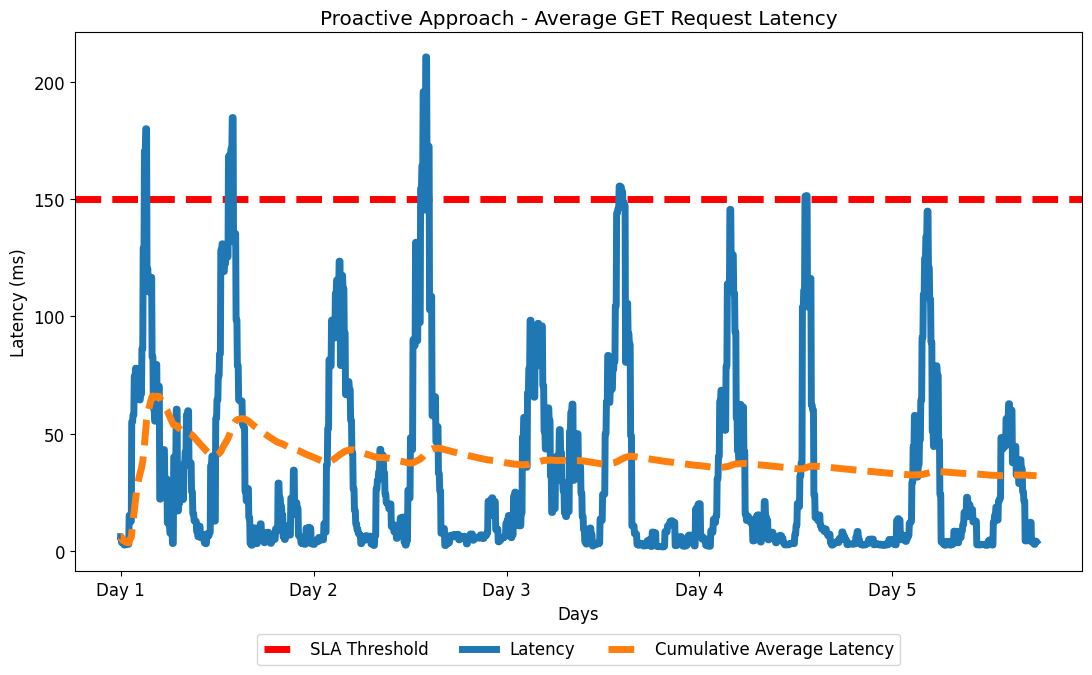
\includegraphics[width=0.6\linewidth]{Figures/Home-Timeline-Proactive-Latency.pdf}
\end{figure}
\end{comment}

\begin{center}
\begin{minipage}{\linewidth}
    \captionof{figure}{PPA proactive autoscaler latency for \textit{home-timeline-service}}
    \label{fig:exp1-proactive-k8s}
    \begin{tikzpicture}
        \begin{axis}[
            height=0.4\linewidth,
            width=\linewidth,
            xmin=0,
            xmax=2460,  % Make xmax 150 above the final xtick
            ymin=0,
            ymajorgrids=true,
            yminorgrids=true,
            xmajorgrids=true,
            xminorgrids=true,
            grid style=dashed,
            xlabel={Time (Days)},
            ylabel={Latency (ms)},
            legend style={at={(0.5,-0.3)},anchor=north,legend columns=-1},
            xticklabels={Day 1, Day 2, Day 3, Day 4, Day 5},
            xtick={570, 1030, 1510, 1950, 2370},
            ytick={0, 75, 150, 225, 300, 375}
        ]
            \addplot+[RoyalBlue, mark=none] table [x=xtick, y=value, col sep=comma] {Data/Home-Timeline-Proactive-Latency-CPU.csv};
            \addplot+[OliveGreen, mark=none] table [x=xtick, y=value, col sep=comma] {Data/Home-Timeline-Proactive-Latency-AVG.csv};
            \draw[red, thick, dashed] (axis cs:0, 150) -- (axis cs:2460, 150);
            \legend{Latency, Cumulative Average Latency}
            \addlegendimage{line width=0.3mm, dashed, color=red}
            \addlegendentry{SLA Threshold}
        \end{axis}
    \end{tikzpicture}
\end{minipage}
\end{center}

Because the autoscaler was purely proactive, it must be a deep LSTM model with several layers and large training epochs. This deep model took more than 50 minutes to properly train and validate for it to predict 24 hours of data, similar to the length of data that our proposed hybrid solution predicted. This is due to the edge architecture's lack of resources and storage compared to the cloud layer. Figure~\ref{fig:exp1-proactive-k8s} shows this in action for the first experiment. Initially, it was observed that the latency continually spiked, causing a large amount of SLA violations, more than what the reactive autoscaler caused. However, after a few days of training, the rolling update structure of the LSTM weights took over, reducing the training time by taking advantage of the early stopping callback in the LSTM model, and managing to stabilize the latency. However, this effect did not always manage to stem the latency overflow, as was shown when the same algorithm was tested using the POST request in Section~\ref{subsec:ch6-proactive-algo}.

While the SLA violations were not as severe as the ones seen in the Default autoscaler baseline, they were comparatively greater than the reactive approach, with the latency exceeding 200 milliseconds for several minutes during the day, which would cause a noticeable delay. The average latency was almost as large as what was seen in the default autoscaler baseline, approaching 50 milliseconds due to the issues inherent in attempting to forecast the entire time-series data curve.\par

\begin{comment}
\begin{figure}[htb]
    \centering
    \caption{PPA Proactive Autoscaler Latency For \textit{compose-post-service}}
    \label{fig:exp2-proactive-k8s}
    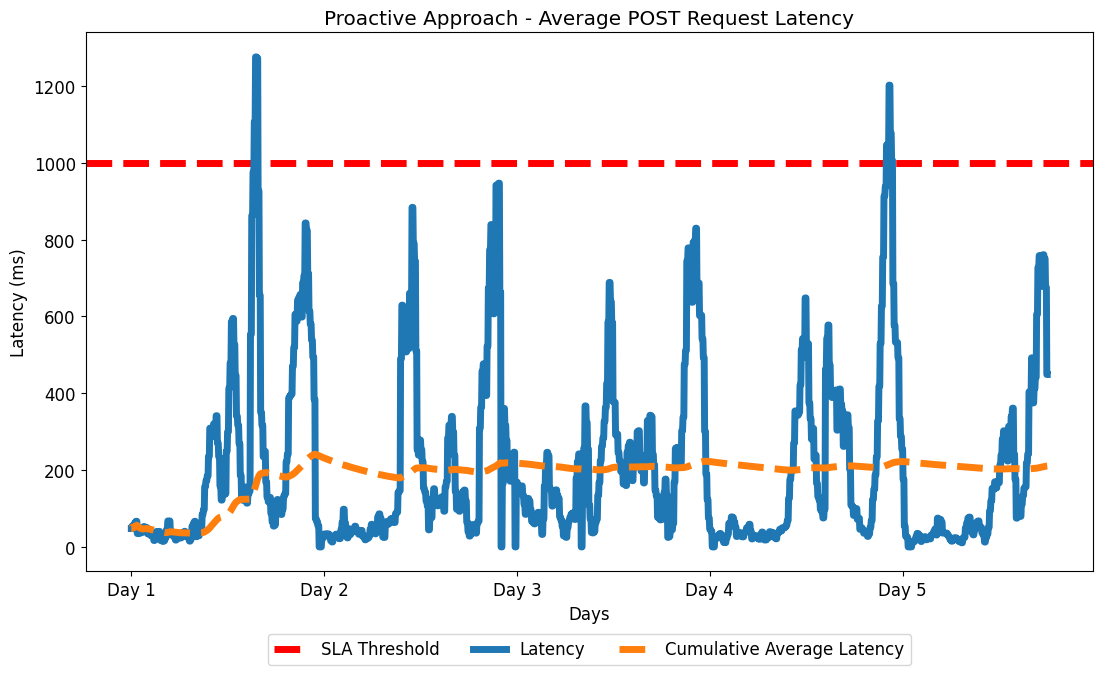
\includegraphics[width=0.6\linewidth]{Figures/Compose-Post-Proactive-Latency.pdf}
\end{figure}
\end{comment}

\begin{center}
\begin{minipage}{\linewidth}
    \captionof{figure}{PPA proactive autoscaler latency for \textit{compose-post-service}}
    \label{fig:exp2-proactive-k8s}
    \begin{tikzpicture}
        \begin{axis}[
            height=0.4\linewidth,
            width=\linewidth,
            xmin=0,
            xmax=2460,  % Make xmax 150 above the final xtick
            ymin=0,
            ymajorgrids=true,
            yminorgrids=true,
            xmajorgrids=true,
            xminorgrids=true,
            grid style=dashed,
            xlabel={Time (Days)},
            ylabel={Latency (ms)},
            legend style={at={(0.5,-0.3)},anchor=north,legend columns=-1},
            xticklabels={Day 1, Day 2, Day 3, Day 4, Day 5},
            xtick={580, 1050, 1510, 1970, 2370}
        ]
            \addplot+[RoyalBlue, mark=none] table [x=xtick, y=value, col sep=comma] {Data/Compose-Post-Proactive-Latency-CPU.csv};
            \addplot+[OliveGreen, mark=none] table [x=xtick, y=value, col sep=comma] {Data/Compose-Post-Proactive-Latency-AVG.csv};
            \draw[red, thick, dashed] (axis cs:0, 1000) -- (axis cs:2460, 1000);
            \legend{Latency, Cumulative Average Latency}
            \addlegendimage{line width=0.3mm, dashed, color=red}
            \addlegendentry{SLA Threshold}
        \end{axis}
    \end{tikzpicture}
\end{minipage}
\end{center}

Figure~\ref{fig:exp2-proactive-k8s} shows the full latency graph for the social network for the second experiment. As can be seen from the data, the latency initially spiked to above 1200 milliseconds, before stabilizing below the SLA threshold. However, one more spike occurred on the last day. Finally, the average latency of the autoscaler performed well, having a value of around 200 milliseconds which was similar to the reactive baseline.\par

Further investigations were conducted in an attempt to explain why these spikes occurred. It was deduced that the first latency spike occurred due to a shortage of training data. The LSTM used by the PPA architecture is extremely complex. Furthermore, apart from data normalization, no other data pre-processing was done such as passing it through the Savitsky-Golay smoothing algorithm. These issues make it more difficult for the forecaster to correctly predict data curves early on in its life cycle. This issue was resolved as more data was added to the training time-series input, however, after a certain point, a threshold was reached where the data was so large, it took a significantly large amount of time for the autoscaler to forecast the workload. This issue led to the latency spike on the final day leading to SLA violations, lasting for several minutes before the autoscaler corrected itself.\par

From these investigations, it can be seen that the proactive auto-scaling approach worked significantly better than the default Kubernetes autoscaler, but performed similarly to the reactive approach. While the social network POST requests were never dropped which would lead to complete system unavailability, the SLA constraints were nonetheless breached, due to the lack of edge layer resources and large training times for the proactive model. Due to issues such as this, the algorithm could not be deemed suitable for edge deployments that were reliant on SLA constraints.\par

\subsection {Proposed Hybrid Autoscaler}
\label{subsec:ch6-hybrid-algo}

\begin{comment}
\begin{figure}[htb]
    \centering
    \caption{Hybrid Autoscaler Latency For \textit{home-timeline-service}}
    \label{fig:exp1-hybrid-k8s}
    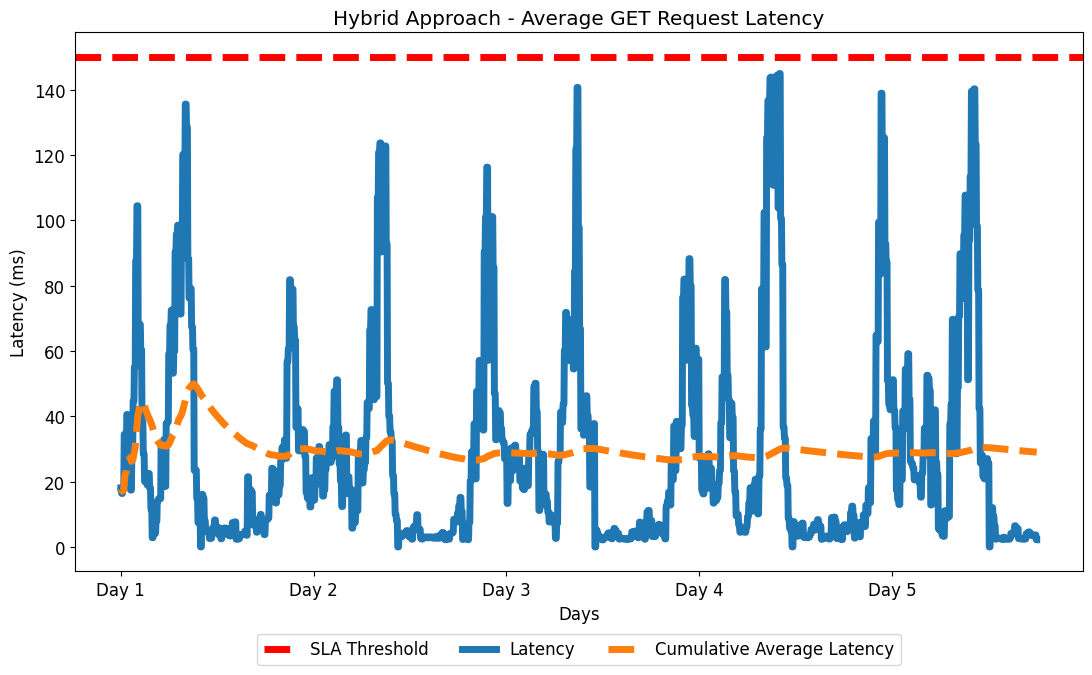
\includegraphics[width=0.6\linewidth]{Figures/Home-Timeline-Hybrid-Latency.pdf}
\end{figure}
\end{comment}

\begin{center}
\begin{minipage}{\linewidth}
    \captionof{figure}{Hybrid autoscaler latency for \textit{home-timeline-service}}
    \label{fig:exp1-hybrid-k8s}
    \begin{tikzpicture}
        \begin{axis}[
            height=0.4\linewidth,
            width=\linewidth,
            xmin=0,
            xmax=2460,  % Make xmax 150 above the final xtick
            ymin=0,
            ymajorgrids=true,
            yminorgrids=true,
            xmajorgrids=true,
            xminorgrids=true,
            grid style=dashed,
            xlabel={Time (Days)},
            ylabel={Latency (ms)},
            legend style={at={(0.5,-0.3)},anchor=north,legend columns=-1},
            xticklabels={Day 1, Day 2, Day 3, Day 4, Day 5},
            xtick={570, 1030, 1510, 1950, 2370}
        ]
            \addplot+[RoyalBlue, mark=none] table [x=xtick, y=value, col sep=comma] {Data/Home-Timeline-Hybrid-Latency-CPU.csv};
            \addplot+[OliveGreen, mark=none] table [x=xtick, y=value, col sep=comma] {Data/Home-Timeline-Hybrid-Latency-AVG.csv};
            \draw[red, thick, dashed] (axis cs:0, 150) -- (axis cs:2460, 150);
            \legend{Latency, Cumulative Average Latency}
            \addlegendimage{line width=0.3mm, dashed, color=red}
            \addlegendentry{SLA Threshold}
        \end{axis}
    \end{tikzpicture}
\end{minipage}
\end{center}

Finally, with the baselines being established in a default, reactive, and proactive approach, the hybrid algorithm was tested on the five days of generated workload. This approach demonstrated how it could mitigate the issues seen in both reactive and proactive auto-scaling approaches. The autoscaler was extremely lightweight, and easy to configure since there was no hyper-parameter tuning required. Building on top of this lightweight, the proactive forecaster was able to forecast the beginning of the workload spike accurately, thus leading to it eliminating the issue of a cold start. The forecaster could not accurately predict the middle and end of the daily workloads, however, this was not an issue, since the reactive algorithm was capable of taking over the auto-scaling process and maintaining the necessary resources to avoid SLA violations. Figure~\ref{fig:exp1-hybrid-k8s} shows the complete latency graph for the GET request experiment.\par

From the graph, it is clear that for the GET request experiment, no SLA violations were present for the duration of the five-day workload. Thus, in this case, the autoscaler controller did not intervene in the LSTM training procedure and modify the hyper-parameters of the forecaster. The average latency experienced by the social network was also comparatively low, achieving results similar to the THPA reactive implementation with the value hovering at around 30 milliseconds. This performance was a significant improvement over the baseline algorithms and demonstrated the efficacy of such a model in an edge architecture deployment.\par

\begin{comment}
\begin{figure}[htb]
    \centering
    \caption{Hybrid Autoscaler Latency For \textit{compose-post-service}}
    \label{fig:exp2-hybrid-k8s}
    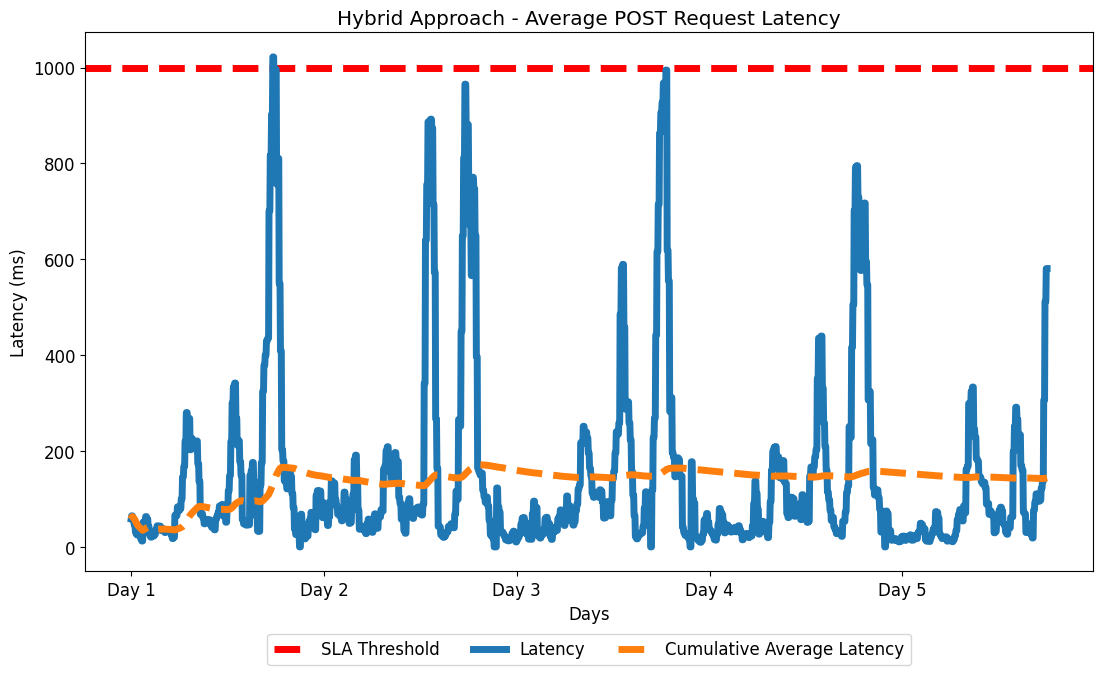
\includegraphics[width=0.6\linewidth]{Figures/Compose-Post-Hybrid-Latency.pdf}
\end{figure}
\end{comment}

\begin{center}
\begin{minipage}{\linewidth}
    \captionof{figure}{Hybrid autoscaler latency for \textit{compose-post-service}}
    \label{fig:exp2-hybrid-k8s}
    \begin{tikzpicture}
        \begin{axis}[
            height=0.4\linewidth,
            width=\linewidth,
            xmin=0,
            xmax=2460,  % Make xmax 150 above the final xtick
            ymin=0,
            ymajorgrids=true,
            yminorgrids=true,
            xmajorgrids=true,
            xminorgrids=true,
            grid style=dashed,
            xlabel={Time (Days)},
            ylabel={Latency (ms)},
            legend style={at={(0.5,-0.3)},anchor=north,legend columns=-1},
            xticklabels={Day 1, Day 2, Day 3, Day 4, Day 5},
            xtick={580, 1050, 1510, 1970, 2370}
        ]
            \addplot+[RoyalBlue, mark=none] table [x=xtick, y=value, col sep=comma] {Data/Compose-Post-Hybrid-Latency-CPU.csv};
            \addplot+[OliveGreen, mark=none] table [x=xtick, y=value, col sep=comma] {Data/Compose-Post-Hybrid-Latency-AVG.csv};
            \draw[red, thick, dashed] (axis cs:0, 1000) -- (axis cs:2460, 1000);
            \legend{Latency, Cumulative Average Latency}
            \addlegendimage{line width=0.3mm, dashed, color=red}
            \addlegendentry{SLA Threshold}
        \end{axis}
    \end{tikzpicture}
\end{minipage}
\end{center}

Figure~\ref{fig:exp2-hybrid-k8s} shows the latency metrics for the five-day workload simulation period for the second POST request experiment. From the graph, it can be clearly seen that only one SLA violation took place on the first day. This was a result of the lack of training data causing an erroneous prediction, an issue faced by the proactive baseline algorithm as well. However, what set this algorithm apart from that baseline was that the reactive autoscaler subsystem was capable of taking over from the proactive subsystem and scaling the resources accordingly. Due to this, the SLA threshold was only breached slightly, peaking at around 1020 milliseconds.\par
After the SLA violation, the autoscaler controller deduced that the training process needed to be kick-started through hyper-parameter tuning. This was done in the next training cycle when the controller provided the forecaster new hyper-parameter values, and as a result, it can be seen that no SLA violations took place on the next day. As a result, the autoscaler controller resets the hyper-parameters to speed up the training process, and even though the latency approached 990 milliseconds on the third day, no further violations took place for the rest of the simulation. The average latency of the whole experiment was also kept below 200 milliseconds, performing slightly better than its reactive and proactive baseline counterparts, and significantly better than the default Kubernetes approach.\par

From these tests, it was clear that the hybrid approach had nearly eliminated the cold start problem very early on in the experiment. The initial difficulties in correctly forecasting the workload peaks were quickly resolved by the autoscaler controller's corrective instructions. All this was done with no user intervention, making the autoscaler extremely autonomous. Furthermore, the algorithm was capable of completing the training within a few minutes, allowing it to finish resource registration quickly. This meant that the CPU utilization of each pod on the nodes never exceeded 100\%, and thus no user API requests were dropped, allowing for full system availability.\par

Based on these results, it was experimentally demonstrated that the proposed hybrid autoscaler performed far better than the baseline algorithms, breaching the SLA threshold in a negligible amount while causing no system unavailability. Thus, the suitability of this hybrid approach for an edge deployment under SLA constraints was proven.

\section{Evaluation of CPU Workload Distribution}
\label{sec:ch6-cpu-workload-eval}

The distribution of CPU $workload$ across the deployment pods was another important metric to factor into the analysis. As a reminder, the goal of the autoscaler was to maximize deployment resources while minimizing deployment costs. Considering the equal importance to be given to both SLA latency and optimization costs as explained in Section~\ref{subsec:ch4-problem-formulation}, and with an autoscaler threshold being set at $\mathcal{A}$, ideally, the distributed workload should hover at $\cfrac{\mathcal{A}}{2}$. When this $workload$ distribution value approaches the value $\mathcal{A}$, it means that not enough pods are being deployed. This results in most if not all active pod resources in the deployment being utilized at full capacity, meaning new requests would need to be queued or even dropped, driving up latency. On the other hand, when $workload$ tends towards the value $0$, it means too many pods have been assigned to the deployment, and thus has been over-scaled. The returns when it comes to latency reduction for such a scaling scenario are extremely low, while the number of idle resource pods being active in the deployment is increasing significantly. This in turn increases the cost of running the underlying edge architecture, making this autoscaler an unprofitable alternative.\par

\begin{comment}
\begin{figure}[htb]
    \centering
    \caption{Autoscaler CPU Workload Distribution Comparison For \textit{home-timeline-service}}
    \label{fig:exp1-cpu-avg-dist}
    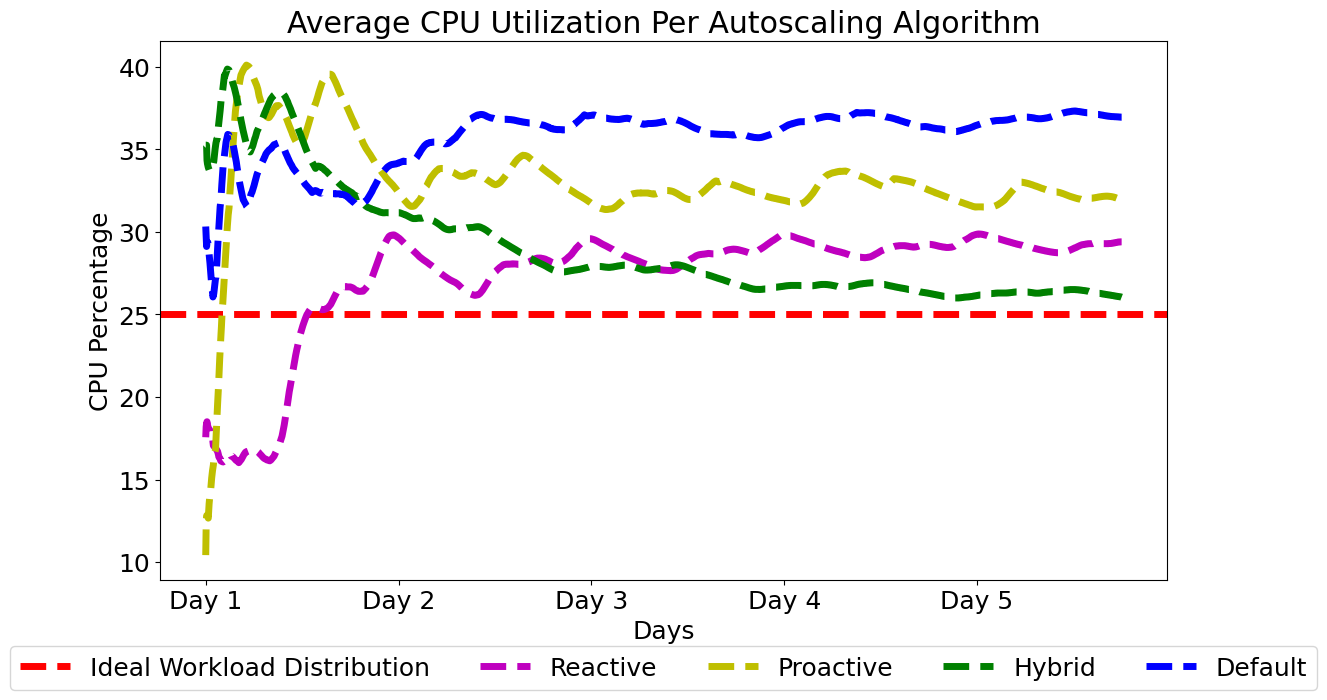
\includegraphics[width=0.6\linewidth]{Figures/Home-Timeline-CPU-Usage.pdf}
\end{figure}
\end{comment}

\begin{center}
\begin{minipage}{\linewidth}
    \captionof{figure}{Autoscaler CPU workload distribution for \textit{home-timeline-service}}
    \label{fig:exp1-cpu-avg-dist}
    \begin{tikzpicture}
        \begin{axis}[
            height=0.4\linewidth,
            width=\linewidth,
            xmin=0,
            xmax=2460,  % Make xmax 150 above the final xtick
            ymin=0,
            ymajorgrids=true,
            yminorgrids=true,
            xmajorgrids=true,
            xminorgrids=true,
            grid style=dashed,
            xlabel={Time (Days)},
            ylabel={CPU Usage (\%)},
            legend style={at={(0.5,-0.3)},anchor=north,legend columns=-1},
            xticklabels={Day 1, Day 2, Day 3, Day 4, Day 5},
            xtick={570, 1030, 1510, 1950, 2370},
            ytick={0, 20, 25, 40}
        ]
            \addplot+[RoyalBlue, mark=none] table [x=xtick, y=value, col sep=comma] {Data/Home-Timeline-CPU-Usage-Default.csv};
            \addplot+[Magenta, mark=none] table [x=xtick, y=value, col sep=comma] {Data/Home-Timeline-CPU-Usage-Reactive.csv};
            \addplot+[Apricot, mark=none] table [x=xtick, y=value, col sep=comma] {Data/Home-Timeline-CPU-Usage-Proactive.csv};
            \addplot+[OliveGreen, mark=none] table [x=xtick, y=value, col sep=comma] {Data/Home-Timeline-CPU-Usage-Hybrid.csv};
            \draw[red, thick, dashed] (axis cs:0, 25) -- (axis cs:2460, 25);
            \legend{Default, Reactive, Proactive, Hybrid}
            \addlegendimage{line width=0.3mm, dashed, color=red}
            \addlegendentry{Ideal CPU Usage}
        \end{axis}
    \end{tikzpicture}
\end{minipage}
\end{center}

For the first experiment, Figure~\ref{fig:exp1-cpu-avg-dist} shows the average CPU utilization $workload$ values of all the deployment pods for the three baseline algorithms and the proposed hybrid solution. As expected, the default Kubernetes horizontal pod autoscaler performs the worst, with the average utilization hovering around 35\%. The proactive forecaster has utilization of approximately 33\%, with it being held back by the forecaster's complexity and resource-intensive training. The reactive approach was the most lightweight autoscaler, and thus performed well with a CPU utilization of around 30\%. Finally, the hybrid autoscaler performed the best of the four compared algorithms, with the utilization of approximately 26\%.\par

In the second experiment with the heavier POST request, the auto-scaling threshold of the experiment $\mathcal{A}$ was set to 60\%. Thus the ideal distributed workload achieved by the autoscaler should be half of the threshold, as calculated in the first experiment. Hence, the distributed workload for this experiment should be $\cfrac{60}{2} = 30\%$

\begin{comment}
\begin{figure}[htb]
    \centering
    \caption{Autoscaler CPU Workload Distribution Comparison For \textit{compose-post-service}}
    \label{fig:exp2-cpu-avg-dist}
    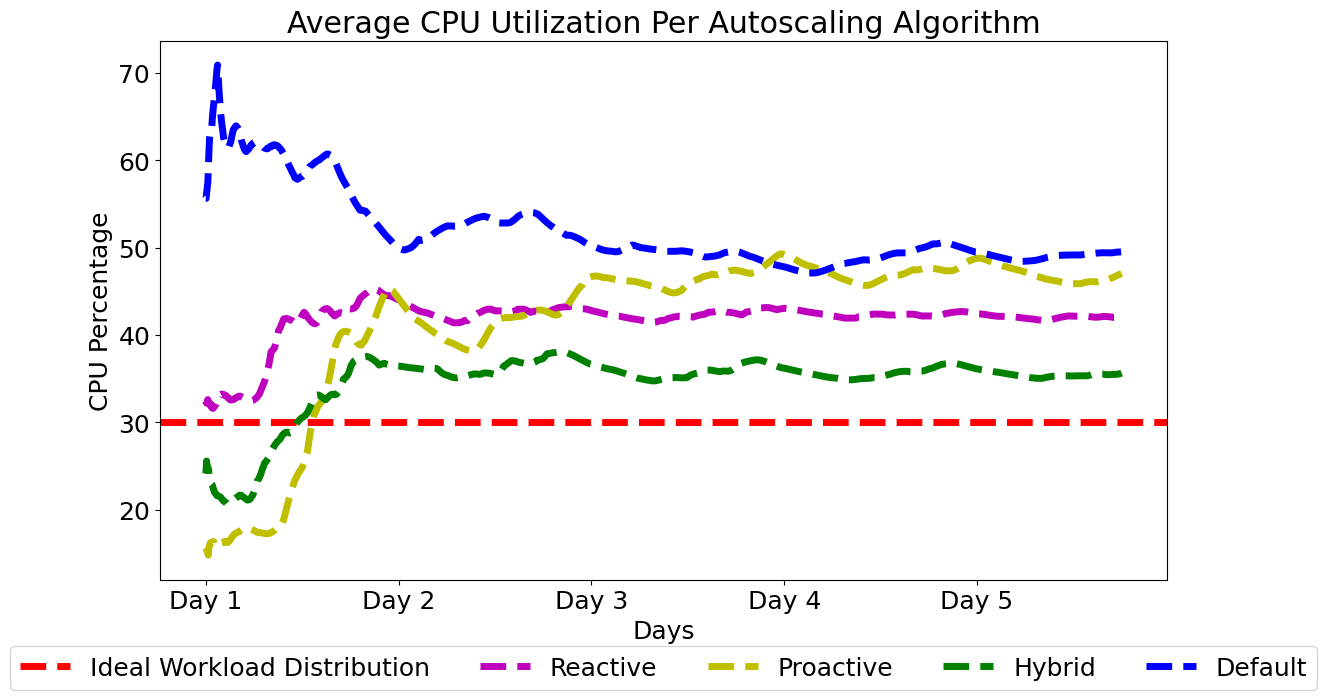
\includegraphics[width=0.6\linewidth]{Figures/Compose-Post-CPU-Usage.pdf}
\end{figure}
\end{comment}

\begin{center}
\begin{minipage}{\linewidth}
    \captionof{figure}{Autoscaler CPU workload distribution for \textit{compose-post-service}}
    \label{fig:exp2-cpu-avg-dist}
    \begin{tikzpicture}
        \begin{axis}[
            height=0.4\linewidth,
            width=\linewidth,
            xmin=0,
            xmax=2460,  % Make xmax 150 above the final xtick
            ymin=0,
            ymajorgrids=true,
            yminorgrids=true,
            xmajorgrids=true,
            xminorgrids=true,
            grid style=dashed,
            xlabel={Time (Days)},
            ylabel={CPU Usage (\%)},
            legend style={at={(0.5,-0.3)},anchor=north,legend columns=-1},
            xticklabels={Day 1, Day 2, Day 3, Day 4, Day 5},
            xtick={580, 1050, 1510, 1970, 2370},
            ytick={0, 15, 30, 45, 60, 75}
        ]
            \addplot+[RoyalBlue, mark=none] table [x=xtick, y=value, col sep=comma] {Data/Compose-Post-CPU-Usage-Default.csv};
            \addplot+[Magenta, mark=none] table [x=xtick, y=value, col sep=comma] {Data/Compose-Post-CPU-Usage-Reactive.csv};
            \addplot+[Apricot, mark=none] table [x=xtick, y=value, col sep=comma] {Data/Compose-Post-CPU-Usage-Proactive.csv};
            \addplot+[OliveGreen, mark=none] table [x=xtick, y=value, col sep=comma] {Data/Compose-Post-CPU-Usage-Hybrid.csv};
            \draw[red, thick, dashed] (axis cs:0, 30) -- (axis cs:2460, 30);
            \legend{Default, Reactive, Proactive, Hybrid}
            \addlegendimage{line width=0.3mm, dashed, color=red}
            \addlegendentry{Ideal CPU Usage}
        \end{axis}
    \end{tikzpicture}
\end{minipage}
\end{center}

Figure~\ref{fig:exp2-cpu-avg-dist} shows the average CPU utilization of the pods for the second experiment, being scaled in the deployment by the three baseline algorithms, along with the proposed hybrid solution. As shown above in Section~\ref{subsec:ch6-default-algo}, the default Kubernetes autoscaler faced issues with system unavailability, with user requests being dropped. This was caused by high CPU usage on the pods, with this being demonstrated by the graph. The average utilization peaked at around 70\% before stabilizing at around 50\% for all the resource pods. However, it is important to note that these resources were not distributed equitably, and thus while some pods had close to 100\% utilization, others had near 0\%.\par

The baseline proactive PPA algorithm performed better than the default Kubernetes autoscaler. While its CPU utilization stabilized fairly quickly to a value of approximately 45\%, this was still far higher than the ideal distributed workload. This was most likely caused by the time it took for the algorithm to forecast data due to the complexity of the LSTM model, which resulted in resources lacking for certain periods of time.\par

The reactive THPA algorithm performed better than the proactive approach, with an average CPU utilization of approximately 42\%. This was achieved due to the intelligent placement of pods in the edge nodes through its traffic-aware algorithm. However, the autoscaler was still prone to the cold start problem, and thus there were several occasions where the CPU workload would peak before the appropriate resources could be assigned. Due to this, the average workload was still far higher than the ideal value.\par

Finally, it can be seen from the graph that the hybrid autoscaler performed better than all three of the baseline algorithms. Its proactive subsystem allowed it to nearly eliminate the cold start problem, while its short training times, and reactive subsystem, allowed the efficient placement of resource pods on the deployment. The average CPU workload quickly stabilized to approximately 35\%, which is far lower than the averages we have seen above for the baseline algorithms, and close to the ideal value of 30\%.\par

Through this comparison, it was clearly demonstrated that for multiple use cases, the hybrid autoscaler managed to scale resources in a manner that both mitigated SLA violations, while doing so in a manner that was both light-weight enough for edge deployments, and inexpensive too.\par

\section{Evaluation of SLA Violation Rates}
\label{sec:ch6-sla-violation-eval}

As demonstrated above, the hybrid autoscaler performed significantly better than the baseline approaches. However, this was only compared using the flexible SLA thresholds. As a reminder, this was the most lenient threshold possible. For a more thorough demonstration, the algorithms needed to be tested on the other possible latency thresholds.\par

To achieve this, all four algorithms were tested again on the moderate and strict SLA violation thresholds for the GET request experiment, as displayed in Table~\ref{tab:experiment-sla-values}. The IoT workload generation algorithm was once again used to generate this, however, this time the workload was run for five days, but auto-scaling was performed only for the last two days. This was done to get the best possible results for all autoscalers regardless of training data length. This resulted in the SLA violation percentage for approximately \num[group-separator={,}]{1020000} GET requests.\par

\begin{comment}
\begin{figure}[htb]
    \centering
    \caption{SLA Violation Percentages For \textit{home-timeline-service}}
    \label{fig:exp1-sla-violation-bar}
    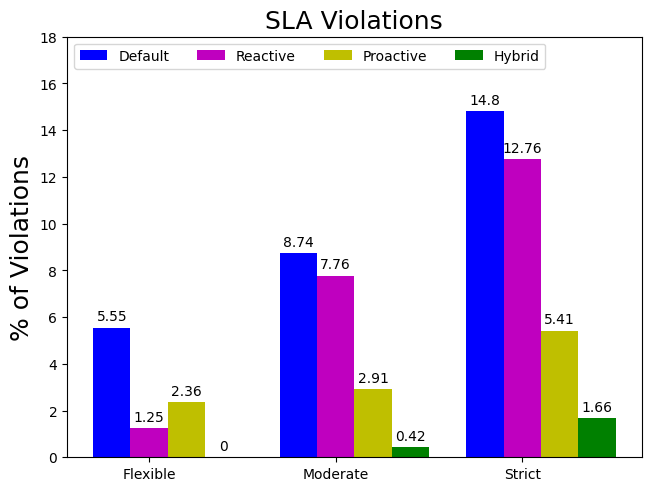
\includegraphics[width=0.6\linewidth]{Figures/Home-Timeline-SLA-Violations.pdf}
\end{figure}

\begin{center}
\begin{minipage}{\linewidth}
    \captionof{figure}{SLA Violation Percentages For \textit{home-timeline-service}}
    \label{fig:exp1-sla-violation-bar}
    \begin{tikzpicture}
        \begin{axis}[
            height=0.4\linewidth,
            width=\linewidth,
            x tick label style={
                /pgf/number format/1000 sep=},
            ylabel=SLA Violations (\%),
            xlabel=SLA Type,
            enlargelimits=0.05,
            legend style={at={(0.3,0.9)},
            anchor=north,legend columns=-1},
            ybar interval=0.8,
            %symbolic x coords = {5,10,50,100,500,1000,DUMMY}
            xticklabels={Flexible, Moderate, Strict, DUMMY},
            xtick={5, 10, 15, 20}
        ]
        \addplot [fill = RoyalBlue]
        coordinates {(5,5.55) (10,8.74) (15,14.8) (20, 0)};
        \addplot [fill = Magenta]
        coordinates {(5,1.25) (10,7.76) (15,12.76) (20, 0)};
        \addplot [fill = Apricot]
        coordinates {(5,2.36) (10,2.91) (15,5.41) (20, 0)};
        \addplot [fill = OliveGreen]
        coordinates {(5,0) (10,0.42) (15,1.66) (20, 0)};
        \legend{Default, Reactive, Proactive, Hybrid}
        \end{axis}
    \end{tikzpicture}
\end{minipage}
\end{center}
\end{comment}

\begin{center}
\begin{minipage}{\linewidth}
    \captionof{figure}{SLA violation percentages for \textit{home-timeline-service}}
    \label{fig:exp1-sla-violation-bar}
    \begin{tikzpicture}
        \begin{axis}[
            height=0.4\linewidth,
            width=\linewidth,
            x tick label style={
                /pgf/number format/1000 sep=},
            ylabel=SLA Violations (\%),
            xlabel=SLA Type,
            enlarge x limits=0.25,
            enlarge y limits=0.15,
            legend style={at={(0.3,0.9)},
            anchor=north,legend columns=-1},
            ybar,
            bar width=22pt,
            symbolic x coords={Flexible, Moderate, Strict},
            xtick=data,
            nodes near coords,
            nodes near coords align={vertical},
        ]
        \addplot [fill = RoyalBlue]
        coordinates {(Flexible,5.55) (Moderate,8.74) (Strict,14.8)};
        \addplot [fill = Magenta]
        coordinates {(Flexible,1.25) (Moderate,7.76) (Strict,12.76)};
        \addplot [fill = Apricot]
        coordinates {(Flexible,2.36) (Moderate,2.91) (Strict,5.41)};
        \addplot [fill = OliveGreen]
        coordinates {(Flexible,0.00) (Moderate,0.42) (Strict,1.66)};
        \legend{Default, Reactive, Proactive, Hybrid}
        \end{axis}
    \end{tikzpicture}
\end{minipage}
\end{center}

Figure~\ref{fig:exp1-sla-violation-bar} shows the SLA violations for the three different categories done on the GET request experiment. The flexible percentages were taken from the data taken from the five-day experiment using the 150 millisecond threshold, while the other two threshold values were extracted from the two-day experiments conducted for each. The default Kubernetes autoscaler performed the worst, with 5.55\% of all requests being above the SLA threshold. The proactive PPA algorithm came next with a violation rate of 2.36\%, with the number of violations being increased due to the complexity of the training model. The reactive THPA algorithm performed well, the low resource deployment, combined with the low overhead of GET requests ensured that it only violated the SLA thresholds of 1.25\% of requests. Finally, as seen above, the hybrid autoscaler performed the best out of the four algorithms, being able to serve all the requests with a 0\% SLA violation rate. This would qualify the hybrid architecture for a ``highly available'' SLA deployment.\par

While the flexible SLA threshold showed impressive results for three out of the four algorithms, the moderate threshold of 125 milliseconds was a more difficult constraint to maintain. The importance of mitigating or eliminating the cold start problem when it came to SLA latency was exposed in this threshold, as the default Kubernetes implementation and the reactive THPA autoscaler showed similarly poor results, violating 8.74\% and 7.76\% of requests respectively. On the contrary, the slower proactive PPA approach was able to demonstrate how mitigating the cold start problem while not being able to eliminate it completely could still have benefits, with the algorithm violating just 2.91\% of requests. Finally, the hybrid autoscaler still achieved the best results. There were violations at the beginning of the experiment, resulting in 0.42\% of requests being above the SLA threshold. However, this was quickly counteracted by the autoscaler controller, which modified the hyper-parameters to stabilize the latency. Once this was achieved, the hyper-parameters were dropped back down to the default values, and the auto-scaling continued as normal.\par

Finally, the strict SLA threshold of 100 milliseconds was tested, which proved extremely difficult to comply with. Once again, the default and reactive autoscalers performed significantly poorly, with 14.8\% and 12.76\% of requests not meeting the SLA threshold respectively. The proactive algorithm distinguished itself from the reactive ones, clearly showing the importance of the cold start problem, by only violating 5.41\% of the requests. However, in this scenario as well, the hybrid algorithm performed substantially better with only 1.66\% of violations. Even though the algorithm would occasionally violate the threshold, the combined approach, along with the controller's heuristic feedback was able to control the violation rate far better than the three baseline approaches. The total number of requests, along with the number of violations is provided in the Table~\ref{tab:exp1-sla-violation-count}.\par

%TC:ignore
\begin{table}
    \caption{SLA violation counts for \textit{home-timeline-service}}\label{tab:exp1-sla-violation-count}
    \centering
    \begin{tabular}{cccc}
        \toprule
        \textbf{Request Counts} & \textbf{Flexible} & \textbf{Moderate} & \textbf{Strict} \\
        \midrule
        Total Requests  & 2,550,000 & 1,220,000 & 1,220,000\\
        \midrule
        Default Violations & \num[group-separator={,}]{141525} & \num[group-separator={,}]{106628} & \num[group-separator={,}]{180560} \\
        Reactive Violations & \num[group-separator={,}]{31875} & \num[group-separator={,}]{94672} & \num[group-separator={,}]{155672} \\
        Proactive Violations & \num[group-separator={,}]{60180} & \num[group-separator={,}]{35502} & \num[group-separator={,}]{66002} \\
        Hybrid Violations & \num[group-separator={,}]{0} & \num[group-separator={,}]{5124} & \num[group-separator={,}]{20252} \\
        \toprule
    \end{tabular}
\end{table}
%TC:endignore

\begin{comment}
\begin{figure}[htb]
    \centering
    \caption{SLA Violation Percentages For \textit{compose-post-service}}
    \label{fig:exp2-sla-violation-bar}
    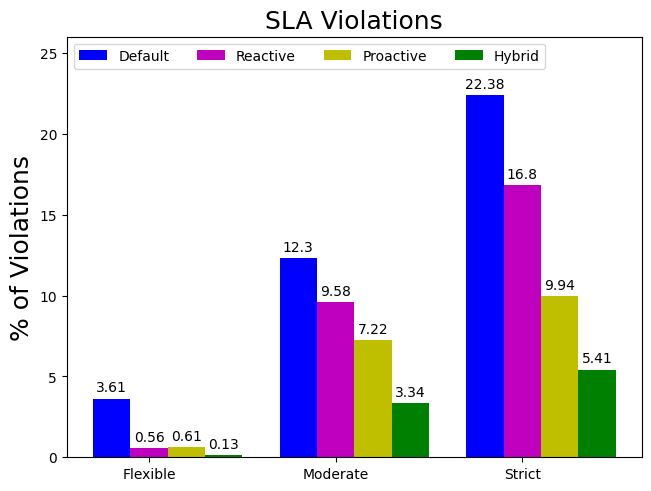
\includegraphics[width=0.6\linewidth]{Figures/Compose-Post-SLA-Violations.pdf}
\end{figure}


\begin{center}
\begin{minipage}{\linewidth}
    \captionof{figure}{SLA Violation Percentages For \textit{compose-post-service}}
    \label{fig:exp2-sla-violation-bar}
    \begin{tikzpicture}
        \begin{axis}[
            height=0.4\linewidth,
            width=\linewidth,
            x tick label style={
                /pgf/number format/1000 sep=},
            ylabel=SLA Violations (\%),
            xlabel=SLA Type,
            enlargelimits=0.05,
            legend style={at={(0.3,0.9)},
            anchor=north,legend columns=-1},
            ybar interval=0.8,
            %symbolic x coords = {5,10,50,100,500,1000,DUMMY}
            xticklabels={Flexible, Moderate, Strict, DUMMY},
            xtick={5, 10, 15, 20},
        ]
        \addplot [fill = RoyalBlue]
        coordinates {(5,3.61) (10,12.3) (15,22.38) (20, 0)};
        \addplot [fill = Magenta]
        coordinates {(5,0.56) (10,9.58) (15,18.8) (20, 0)};
        \addplot [fill = Apricot]
        coordinates {(5,0.61) (10,7.22) (15,9.94) (20, 0)};
        \addplot [fill = OliveGreen]
        coordinates {(5,0.13) (10,3.34) (15,5.41) (20, 0)};
        \legend{Default, Reactive, Proactive, Hybrid}
        \end{axis}
    \end{tikzpicture}
\end{minipage}
\end{center}
\end{comment}

\begin{center}
\begin{minipage}{\linewidth}
    \captionof{figure}{SLA violation percentages for \textit{compose-post-service}}
    \label{fig:exp2-sla-violation-bar}
    \begin{tikzpicture}
        \begin{axis}[
            height=0.4\linewidth,
            width=\linewidth,
            x tick label style={
                /pgf/number format/1000 sep=},
            ylabel=SLA Violations (\%),
            xlabel=SLA Type,
            enlarge x limits=0.25,
            enlarge y limits=0.15,
            legend style={at={(0.3,0.9)},
            anchor=north,legend columns=-1},
            ybar,
            bar width=22pt,
            symbolic x coords={Flexible, Moderate, Strict},
            xtick=data,
            nodes near coords,
            nodes near coords align={vertical},
        ]
        \addplot [fill = RoyalBlue]
        coordinates {(Flexible,3.61) (Moderate,12.3) (Strict,22.38)};
        \addplot [fill = Magenta]
        coordinates {(Flexible,0.56) (Moderate,9.58) (Strict,18.8)};
        \addplot [fill = Apricot]
        coordinates {(Flexible,0.61) (Moderate,7.22) (Strict,9.94)};
        \addplot [fill = OliveGreen]
        coordinates {(Flexible,0.13) (Moderate,3.34) (Strict,5.41)};
        \legend{Default, Reactive, Proactive, Hybrid}
        \end{axis}
    \end{tikzpicture}
\end{minipage}
\end{center}

Figure~\ref{fig:exp2-sla-violation-bar} depicts the SLA violations for all four algorithms for the three SLA categories done on the POST request experiment. Once again, the flexible percentages were derived from the data taken during the five-day experiment using the 1000 millisecond threshold, while the moderate (900 milliseconds) and strict (800 milliseconds) violations were derived from the two-day workload above.\par

As seen above, for the flexible category, the default Kubernetes autoscaler performed the worst, with 3.61\% of the total requests resulting in an SLA violation. This also includes the requests which resulted in an error due to being dropped by the social network. The reactive and proactive algorithms performed comparatively similarly to each other, achieving a 0.56\% and 0.61\% violation rate respectively. The lenient threshold means that the proactive algorithm is unable to display its benefits when it comes to mitigating the cold start problem as compared to the reactive approach. Finally, the hybrid approach achieved a 0.13\% SLA violation rate. This results in approximately 99.9\% availability for the system, indicating that even for a difficult auto-scaling task such as for the POST request scenario, the hybrid algorithm is capable of achieving near ``high availability''.\par

The moderate SLA threshold proved far more difficult for all the algorithms to adhere to. Once again, the default Kubernetes autoscaler performed the worst of all four, failing to adhere to the SLA constraint for 12.3\% of the requests. Here, the proactive autoscaler was able to demonstrate the importance of mitigating the issue of cold start. It was able to achieve a 7.22\% of SLA violations, which was far lower than the 9.58\% seen for the reactive autoscaler. However, once again, the hybrid solution proved to be the most capable of auto-scaling in this scenario, achieving an SLA violation rate of just 3.34\%.

Finally, the extremely challenging strict threshold was tested. The default Kubernetes autoscaler was unable to cope with such a threshold, violating this threshold for over one-fourth of the requests, with a 22.38\% violation rate. Once again, the proactive algorithm outperformed the reactive one, achieving a 9.94\% violation rate as compared to the 18.8\% of the reactive algorithm. Finally, the hybrid algorithm performed significantly better than all three baselines yet again, with a violation rate of just 5.41\%.\par

This meant that over the two experiments and three SLA thresholds, the hybrid approach served a minimum of 94.5\% of all requests in an SLA-compliant manner in the worst-case scenario while serving 100\% of them in the best case. Through this thorough testing and experimentation, the algorithm displayed its robustness and adaptability while requiring little to no customization by the user to achieve excellent results. The total number of requests, along with the number of request violations for the second experiment is displayed in Table~\ref{tab:exp2-sla-violation-count}.\par

%TC:ignore
\begin{table}
    \caption{SLA violation counts for \textit{compose-post-service}}\label{tab:exp2-sla-violation-count}
    \centering
    \begin{tabular}{cccc}
        \toprule
        \textbf{Request Counts} & \textbf{Flexible} & \textbf{Moderate} & \textbf{Strict} \\
        \midrule
        Total Requests  & 2,550,000 & 1,220,000 & 1,220,000\\
        \midrule
        Default Violations & \num[group-separator={,}]{92055} & \num[group-separator={,}]{150060} & \num[group-separator={,}]{273036} \\
        Reactive Violations & \num[group-separator={,}]{14280} & \num[group-separator={,}]{116876} & \num[group-separator={,}]{229360} \\
        Proactive Violations & \num[group-separator={,}]{15555} & \num[group-separator={,}]{88084} & \num[group-separator={,}]{121268} \\
        Hybrid Violations & \num[group-separator={,}]{3315} & \num[group-separator={,}]{40748} & \num[group-separator={,}]{66002} \\
        \toprule
    \end{tabular}
\end{table}
%TC:endignore

Thus for the two experiments, and on three different SLA thresholds, it can be comprehensively concluded that the hybrid approach proved to be the best autoscaler when it came to an edge deployment with minimal resources available. Furthermore, the algorithm was adaptable and able to display considerably improved performance in comparison with other reactive and proactive approaches. It was able to achieve this with minimal parameter configurations required by the user, and minimizing the cost of deploying and maintaining the edge architecture.

\clearpage

\def\chaptertitle{Conclusion}

\lhead{\emph{\chaptertitle}}

\chapter{\chaptertitle}
\label{ch:conclusion}

\section{Overview}
\label{sec:ch7-overview}

In conclusion, the thesis provides a novel, lightweight, and SLA-compliant approach to autoscale resources on a micro-service deployed on an edge architecture. In comparison to other state-of-the-art autoscalers, the algorithm performs considerably better in terms of SLA violation as well as resource usage.\par

The autoscaler architecture is open source \footnote{\url{https://github.com/suhridgupta/K8s-Proactive-Forecaster}} \footnote{\url{https://github.com/suhridgupta/jaeger-scraper}}, and provides a framework to further develop more sophisticated auto-scaling solutions. These extensions will be discussed in section \ref{subsec:ch7-extensions}.\par

Furthermore, the outcome of this thesis is being used to develop two publications. The first is a research paper which is aimed to be published in the IEEE Cloud Conference \footnote{\url{https://ieeexplore.ieee.org/xpl/conhome/1002911/all-proceedings}}. The paper will focus on cloud-edge layer deployment of Kubernetes, how the hybrid autoscaler fits into this architecture to provide SLA-compliance, as well as the mathematical modeling of the problem along with the performance evaluation.\par

The second is an implementation framework publication which is aimed to be published in the Future Generation Computer Systems \footnote{\url{https://www.sciencedirect.com/journal/future-generation-computer-systems}} journal. The autoscaler will be presented as an extendable framework on top of Kubernetes. The publication will discuss the modifications made to the autoscaler to make it SLA-compliant, and the methods by which users can develop their own auto-scaling policies using the hybrid autoscaler as a plug-in.\par

\section{Contributions}
\label{sec:ch7-contribution}

The contributions of this thesis can be broken down into three main segments: identifying the major bottlenecks of auto-scaling on an edge deployment in comparison to a typical cloud architecture, designing a novel hybrid auto-scaling architecture which is built primarily of the edge paradigm, and streamlining the forecaster used by the hybrid autoscaler, thus making it capable of running on resource-limited edge deployments.\par

Through the extensive literature review conducted in chapter \ref{ch:lit-review}, the key aspects which make the typical cloud-based hybrid autoscalers infeasible  for edge deployments were identified, this being a lack of computing and storage resources in the edge layer as compared to the cloud layer, the difficulty in hyper-parameter tuning, and the complexity of the forecast models driving up the model training time. With these issues identified, a hybrid auto-scaling architecture was proposed which addressed all the reported bottlenecks, and was capable of scaling resources in the edge environment in an SLA-compliant manner.\par

Based on the investigation of existing hybrid autoscalers conducted in section \ref{sec:ch3-hybrid-solutions}, all existing autoscalers are not edge architecture compliant, as they were too resource intensive, or not SLA-compliant, or both. Thus the hybrid architecture proposed in this thesis was a novel approach which maintained SLA compliance and ease-of-deployment on edge paradigms. It did so by combining a reactive autoscaler with a streamlined proactive model built using LSTM. To eliminate the difficult hyper-parameter tuning process, the autoscaler was built with a heuristic approach in mind, where the parameters were automatically fine-tuned in case any SLA violations were seen in the data.\par

Finally, the autoscaler was tested on a production-ready social network micro-service deployment, and the results were compared with other cutting-edge autoscalers. The results showed that the proposed autoscaler has a maximum SLA violation rate of $5.41\%$, as compared to a maximum of $18.8-22.38\%$ for the other state-of-the-art autoscalers.\par

The tests were further able to demonstrate that the autoscaler was capable of significantly reducing SLA violations while also keeping the overall cost related to deploying the container orchestration resources on a cloud provider as low as possible. It does so by assigning resources in a manner which keeps the utilized resources at approximately half of the configured auto-scaling threshold.\par

Based on the work done in this thesis, the research questions stated in section \ref{sec:ch1-problem-overview} can be conclusively answered.

\begin{itemize}
    \item \textbf{\textit{RQ1:}} The work done in this thesis successfully integrated reactive and proactive auto-scaling algorithms to develop a hybrid autoscaler tailored for edge computing architectures. The autoscaler was both light weight, allowing it to be run on the edge layer, while also eliminating the requirement for tedious and complicated hyper-parameter tuning seen in most proactive auto-scaling solutions.
    \item \textbf{\textit{RQ2:}} The work done in this thesis successfully demonstrated that the autoscaler exceeded the SLA compliance capabilities of state-of-the-art reactive and proactive auto-scaling solutions for edge computing, while minimizing the cost of deploying the application.
\end{itemize}

\section{Future Work}
\label{sec:ch7-future-work}

\subsection{Current Limitations}
\label{subsec:ch7-limitations}

Several assumptions have been made when conducting the experiments, the primary ones being that only a single SLA metric was used to design the heuristic model, the auto-scaling approach was limited to horizontally scaling resources, and the forecaster used a simple LSTM machine learning model using a single parameter. In the next section, some extensions to improve the robustness of the hybrid autoscaler is proposed, along with some approaches to improve the efficiency and accuracy of its forecasts.\par

\subsection{Proposed Extensions}
\label{subsec:ch7-extensions}

\subsubsection{Alternative Auto-scaling Approaches}
\label{subsubsec:ch7-alternate-auto}

The proposed hybrid model autoscales resources in a strictly horizontal manner. One of the underlying assumptions was that no other auto-scaling was to take place while the micro-service deployments were being stress tested. This meant that only the number of deployment replicas were either increased or decreased, keeping all other parameters untouched.\par

A future extension to this thesis would be to configure the algorithm such that it can attempt other forms of auto-scaling too. For example, the hybrid model may be configured as a Vertical Pod Autoscaler (VPA) instead. In this approach, the reactive autoscaler will modify the CPU reservations for the deployments, while leaving the number of deployment replicas untouched. Similarly, the proactive forecaster will attempt to predict the future CPU workload, and autoscale beforehand accordingly. The benefit of such an approach is that the forecaster already works in a similar manner, predicting future CPU workloads, and thus only minor modifications would be required to configure the hybrid HPA into a VPA.\par

A more challenging extension would be to transform the hybrid model into a Cluster Autoscaler. In the cluster autoscaler, the container orchestration platform will adjust the size of the cluster (edge nodes) when one of the following conditions holds:

\begin{itemize}
    \item There are deployment replicas in the cluster which are currently un-assigned to any node due to insufficient resources.
    \item There are nodes in the cluster that have not had sufficient utilization of resources for a configured period of time, and as such, their active deployment replicas can be re-scheduled on to other nodes, after which the node can be decommissioned to free up resources.
\end{itemize}

While converting this autoscaler architecture for cloud computing is a straightforward process, due to the inherent homogeneity of the paradigm, it is much more difficult for an edge computing approach. Since different resource workloads are exerted on the various edge nodes, care needs to be taken when re-scheduling deployment replicas to other nodes, as well as decommissioning nodes. This process needs to be done in an intelligent manner such that the overall latency of the micro-service does not increase due to an added distance between the end user and the modified edge layer architecture. Therefore the auto-scaling controller must be modified in a way such that it can identify nodes nearby to it such that it can re-assign replicas.

\subsubsection{Multi-Variate Forecaster}
\label{subsubsec:ch7-multi-variate}

The forecaster used in the hybrid autoscaler is a uni-variate LSTM model. This means that at any given time, only one variable is changing. Therefore the input is a one-dimensional array. An extension can be made to the forecaster to convert it into a multi-variate model. In this approach, multiple variables are being modified at a given time, thus the input to the model is a more complex two-dimensional array.\par

The benefit of a multi-variate approach is that a more holistic auto-scaling decision can be made using this. For example, the VPA model discussed in section \ref{subsubsec:ch7-alternate-auto}, the reactive and proactive algorithms can be modified to autoscale on both CPU and memory utilization. The forecaster can then take the CPU and memory time-series data as input, and output the forecast for both. Through this, the autoscaler can form a better picture of the resource utilization of the micro-service, identifying bottlenecks and mitigating them.\par

The drawback of such an approach is that the proactive forecaster training times will significantly increase due to two reasons. The first one is the additional complexity of the input as well as output. Due to the multiple variables needing to be trained and validated on, more epochs are required, along with each epoch taking longer to evaluate. Furthermore the validation process will take longer as well. The second cause is due to the memory time-series not being as predictable as the CPU utilization. In the CPU utilization graphs of the deployments as seen in figure \ref{fig:lstm-init-data}, the workload forms clear and identifiable patterns which can be easily recognized by the model. Memory is far more variable, with sudden peaks and falls depending on several of the processes running in the deployment. Thus the autoscaler must concomitantly be made as complex, with far larger and deeper neural network architectures.\par

Due to this drawback, further research is required to verify the feasibility of using a multi-variate machine learning model to forecast workloads, and to confirm whether or not it is suitable for an edge deployment.

\begin{comment}
\subsubsection{Auto-regressive Forecaster}
\label{subsubsec:ch7-auto-regressive}

So far, the proactive forecaster implemented in the hybrid solution, along with the enhancements discussed above, have predicted the entire output in a single step. There is an alternative method of forecasting, where the model decomposes this prediction process into individual steps. By doing so, at each step the model's outputs can be fed back into itself, making the next prediction dependant on the output of the previous one. Figure \ref{fig:auto-regressive-lstm} shows a simplified overview of this process.\par

\begin{figure}[htb]
    \centering
    \caption{Auto-Regressive LSTM Prediction, courtesy of Tensorflow \cite{autoregressivelstm}}
    \label{fig:auto-regressive-lstm}
    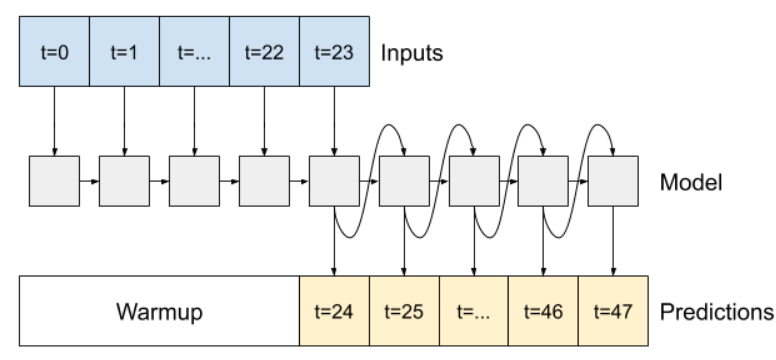
\includegraphics[width=0.6\linewidth]{Figures/Auto-Regressive-LSTM.png}
\end{figure}

There are benefits in using an auto-regressive approach, the training window, which is the number of previous steps which the LSTM model uses to predict the output, can be drastically lowered for large outputs. This is because the model is no longer predicting a large output in one shot, but unit predictions in an iterative process. Another benefit is that the model can re-use the previously predicted data as training input for the subsequent prediction steps, which can potentially increase the accuracy of the model. Lastly, this model is highly customizable. Whereas the hybrid approach proposed in this algorithm predicts 24 hours of data points, the auto-regressive approach can be set to output predictions of any length.\par

However this added complexity requires far larger usage of resources. Furthermore, the iterative prediction process can result in a lack of parallel resource usage, meaning it takes far longer to predict the same amount of data as seen in proposed hybrid solution. Further research is required to verify if such an auto-regressive model is feasible for an edge deployment.
\end{comment}

\subsubsection{Multi-SLA Constraints}
\label{subsubsec:ch7-multi-sla}

Another modification which can be made to the hybrid autoscaler is to support the use of multiple SLA constraints. Currently, the autoscaler only takes into account a single metric, and bases its heuristic feedback algorithm on it. By modifying this into a multi-parameter model, the autoscaler can keep a track of several metrics, and if a violation occurs on any one of them, can tune the auto-scaling process accordingly.\par

Such a modification opens up several other possibilities too. Each SLA metric can be given its own weight to denote importance. The current hybrid autoscaler only considers a single action of tuning the forecaster hyper-parameter variables on SLA violation occurrences. By making it a multi-SLA model with different weights attached, the hybrid autoscaler can intelligently decide what actions to take when on different scenarios such as urgent and mild SLA violations.\par

This adds further complexity to the autoscaler however, and the constant tuning of forecast parameters may cause issues such as a drop in prediction accuracy and under-fitting / over-fitting. Thus a balance needs to be struck in the actions to be taken on SLA constraints being violated, and additional cooldowns need to be implemented on the frequency of such actions being implemented.

\begin{comment}
\subsubsection{Alternative LSTM Configurations}
\label{subsubsec:ch7-advanced-lstm-config}

A \textit{classic LSTM} model, similar to the one implemented by Hochreiter and Schmidhuber \cite{hochreiter1997long} was used in this research. As explained in section \ref{sec:ch2-time-series}, this consists of memory cells, forget gates, input gates, and output gates. The strength of such a model lies in its ability to extract features from the data with varying time lags to create long-range dependencies. This model however has several extensions, some of which are discussed below.\par

\textit{Bidirectional LSTM} \cite{graves2005framewise} is an extension of the classic LSTM architecture. This model encompasses bi-directional processing to enable the capture of information from both the past and future inputs. This is done using two separate LSTM layers, a forward LSTM layer which processes the input from beginning to end, and a backward LSTM layer which processes the input in reverse. The outputs of both layers are concatenated at each step, thus capturing a richer feature set from the data to make a more accurate forecast. This approach is resource intensive, however, and may see limited improvements over the classic approach, since Bidirectional LSTM models are best suited for applications where understanding the sequential context in both directions is crucial \cite{breuel2015benchmarking}.\par

\textit{LSTM with attention mechanisms} \cite{zheng2021understanding} transforms the classic LSTM to allow the model to focus on specific features of the data. This architecture incorporates attention weights that compute the importance of each input at a given training iteration. These attention weights are adjusted dynamically during the training process based on the relevance of each input element for the current prediction. By focusing on specific sections of the input, the model can better capture dependencies in lengthy input data series without being overwhelmed, resulting in higher prediction accuracy \cite{zhou2020comparison}. There are some drawbacks to applying such an approach to an edge micro-service however, since this model is best used for capturing fine-grained dependencies in the time-series data. Such detailed dependencies are not required in a hybrid model, since the reactive portion of the autoscaler can shoulder most of the auto-scaling responsibility. Thus further research needs to be carried out in evaluating the benefits of using such a proactive forecaster approach.\par

Finally, a model which may provide faster training times is the \textit{Gated Recurrent Unit} (GRU) \cite{chung2014empirical}. The GRU combines the input and forget gates of the classic LSTM into a unified gate. Similarly, the cell state and hidden output are also combined into a combined hidden state layer. Finally, the model contains an internal hidden state. Through these modifications, the GRU is able to efficiently capture dependencies and features in sequential data, making them particularly useful for resource-constrained real-time applications, such as edge deployments \cite{yang2020lstm}. Using this model may eliminate some of the performance drawbacks seen in multi-variate forecasters in section \ref{subsubsec:ch7-multi-variate} making it a viable alternative for implementing such a system.\par
\end{comment}

\addtocontents{toc}{\vspace{2em}}

%TC:ignore
%\appendix
%\input{appendices/data.tex}
%\input{appendices/programs.tex}
%\chapter{Appendix}

%TC:endignore

\addtocontents{toc}{\vspace{2em}}
\backmatter

\lhead{\emph{Bibliography}}
\bibliographystyle{unsrtnat}
\bibliography{Thesis}
\label{bibliography}

\end{document}
